\documentclass[11pt,a4paper]{article}

% Packages
\usepackage{graphicx}  % driver auto-detected (Tectonic/XeTeX); no dvipdfmx option
\usepackage{amsmath}
\usepackage{amssymb}
\usepackage{authblk}
\usepackage{bm}
\usepackage{caption}
\usepackage{color}
\usepackage[T1]{fontenc}
\usepackage[colorlinks=true]{hyperref}
\usepackage{mathtools}
\usepackage[numbers]{natbib}
\usepackage{stmaryrd}
\usepackage{tgtermes}

% packages
% \usepackage[linesnumbered,ruled]{algorithm2e}  % unused by this paper; absent from Wisteria texlive
\usepackage{amsmath}
\usepackage{amssymb}
\usepackage{amsthm}
\usepackage{bm}
\usepackage{booktabs}
\usepackage[font=footnotesize,labelfont=bf]{caption}
\usepackage[capitalize,nameinlink]{cleveref}
\usepackage{color}
% \usepackage{dsfont}  % unused by this paper; absent from Wisteria texlive
\usepackage[T1]{fontenc}
\usepackage{mathtools}
\usepackage{mathrsfs}
% \usepackage{multirow}  % unused by this paper; absent from Wisteria texlive
\usepackage{pifont}
\usepackage{rotating}
% \usepackage[group-separator={,},group-minimum-digits={3}]{siunitx}  % unused; absent from Wisteria texlive
\usepackage{subcaption}
\usepackage{tabularx}
\usepackage{tikz}
% \usepackage{wrapfig}  % unused by this paper; absent from Wisteria texlive

% config
\hypersetup{
  colorlinks=true,
  linkcolor={red!15!green!35!blue!95},
  citecolor={green!50!black},
  urlcolor={red!50!black}
}

% algorithm2e config (disabled with the package above)
% \DontPrintSemicolon
% \SetArgSty{textnormal}
% \SetKwInOut{Input}{Input}
% \SetKwInOut{Output}{Output}
% \SetKwComment{Comment}{$\triangleright$\ }{}

% universal
\renewcommand{\tilde}{\widetilde}
\renewcommand{\hat}{\widehat}
\newcommand{\Acal}{\mathcal{A}}
\newcommand{\Bcal}{\mathcal{B}}
\newcommand{\Ccal}{\mathcal{C}}
\newcommand{\Dcal}{\mathcal{D}}
\newcommand{\Ecal}{\mathcal{E}}
\newcommand{\Fcal}{\mathcal{F}}
\newcommand{\Gcal}{\mathcal{G}}
\newcommand{\Hcal}{\mathcal{H}}
\newcommand{\Ical}{\mathcal{I}}
\newcommand{\Jcal}{\mathcal{J}}
\newcommand{\Kcal}{\mathcal{K}}
\newcommand{\Lcal}{\mathcal{L}}
\newcommand{\Mcal}{\mathcal{M}}
\newcommand{\Ncal}{\mathcal{N}}
\newcommand{\Ocal}{\mathcal{O}}
\newcommand{\Pcal}{\mathcal{P}}
\newcommand{\Qcal}{\mathcal{Q}}
\newcommand{\Rcal}{\mathcal{R}}
\newcommand{\Scal}{\mathcal{S}}
\newcommand{\Tcal}{\mathcal{T}}
\newcommand{\Ucal}{\mathcal{U}}
\newcommand{\Vcal}{\mathcal{V}}
\newcommand{\Wcal}{\mathcal{W}}
\newcommand{\Xcal}{\mathcal{X}}
\newcommand{\Ycal}{\mathcal{Y}}
\newcommand{\Zcal}{\mathcal{Z}}
\newcommand{\Abb}{\mathbb{A}}
\renewcommand{\Bbb}{\mathbb{B}}
\newcommand{\Cbb}{\mathbb{C}}
\newcommand{\Dbb}{\mathbb{D}}
\newcommand{\Ebb}{\mathbb{E}}
\newcommand{\Fbb}{\mathbb{F}}
\newcommand{\Gbb}{\mathbb{G}}
\newcommand{\Hbb}{\mathbb{H}}
\newcommand{\Ibb}{\mathbb{I}}
\newcommand{\Jbb}{\mathbb{J}}
\newcommand{\Kbb}{\mathbb{K}}
\newcommand{\Lbb}{\mathbb{L}}
\newcommand{\Mbb}{\mathbb{M}}
\newcommand{\Nbb}{\mathbb{N}}
\newcommand{\Obb}{\mathbb{O}}
\newcommand{\Pbb}{\mathbb{P}}
\newcommand{\Qbb}{\mathbb{Q}}
\newcommand{\Rbb}{\mathbb{R}}
\newcommand{\Sbb}{\mathbb{S}}
\newcommand{\Tbb}{\mathbb{T}}
\newcommand{\Ubb}{\mathbb{U}}
\newcommand{\Vbb}{\mathbb{V}}
\newcommand{\Wbb}{\mathbb{W}}
\newcommand{\Xbb}{\mathbb{X}}
\newcommand{\Ybb}{\mathbb{Y}}
\newcommand{\Zbb}{\mathbb{Z}}
\newcommand{\Ads}{\mathds{A}}
\newcommand{\Bds}{\mathds{B}}
\newcommand{\Cds}{\mathds{C}}
\newcommand{\Dds}{\mathds{D}}
\newcommand{\Eds}{\mathds{E}}
\newcommand{\Fds}{\mathds{F}}
\newcommand{\Gds}{\mathds{G}}
\newcommand{\Hds}{\mathds{H}}
\newcommand{\Ids}{\mathds{I}}
\newcommand{\Jds}{\mathds{J}}
\newcommand{\Kds}{\mathds{K}}
\newcommand{\Lds}{\mathds{L}}
\newcommand{\Mds}{\mathds{M}}
\newcommand{\Nds}{\mathds{N}}
\newcommand{\Ods}{\mathds{O}}
\newcommand{\Pds}{\mathds{P}}
\newcommand{\Qds}{\mathds{Q}}
\newcommand{\Rds}{\mathds{R}}
\newcommand{\Sds}{\mathds{S}}
\newcommand{\Tds}{\mathds{T}}
\newcommand{\Uds}{\mathds{U}}
\newcommand{\Vds}{\mathds{V}}
\newcommand{\Wds}{\mathds{W}}
\newcommand{\Xds}{\mathds{X}}
\newcommand{\Yds}{\mathds{Y}}
\newcommand{\Zds}{\mathds{Z}}
\newcommand{\Abf}{\mathbf{A}}
\newcommand{\Bbf}{\mathbf{B}}
\newcommand{\Cbf}{\mathbf{C}}
\newcommand{\Dbf}{\mathbf{D}}
\newcommand{\Ebf}{\mathbf{E}}
\newcommand{\Fbf}{\mathbf{F}}
\newcommand{\Gbf}{\mathbf{G}}
\newcommand{\Hbf}{\mathbf{H}}
\newcommand{\Ibf}{\mathbf{I}}
\newcommand{\Jbf}{\mathbf{J}}
\newcommand{\Kbf}{\mathbf{K}}
\newcommand{\Lbf}{\mathbf{L}}
\newcommand{\Mbf}{\mathbf{M}}
\newcommand{\Nbf}{\mathbf{N}}
\newcommand{\Obf}{\mathbf{O}}
\newcommand{\Pbf}{\mathbf{P}}
\newcommand{\Qbf}{\mathbf{Q}}
\newcommand{\Rbf}{\mathbf{R}}
\newcommand{\Sbf}{\mathbf{S}}
\newcommand{\Tbf}{\mathbf{T}}
\newcommand{\Ubf}{\mathbf{U}}
\newcommand{\Vbf}{\mathbf{V}}
\newcommand{\Wbf}{\mathbf{W}}
\newcommand{\Xbf}{\mathbf{X}}
\newcommand{\Ybf}{\mathbf{Y}}
\newcommand{\Zbf}{\mathbf{Z}}
\newcommand{\abf}{\mathbf{a}}
\newcommand{\bbf}{\mathbf{b}}
\newcommand{\cbf}{\mathbf{c}}
\newcommand{\dbf}{\mathbf{d}}
\newcommand{\ebf}{\mathbf{e}}
\newcommand{\fbf}{\mathbf{f}}
\newcommand{\gbf}{\mathbf{g}}
\newcommand{\hbf}{\mathbf{h}}
\newcommand{\ibf}{\mathbf{i}}
\newcommand{\jbf}{\mathbf{j}}
\newcommand{\kbf}{\mathbf{k}}
\newcommand{\lbf}{\mathbf{l}}
\newcommand{\mbf}{\mathbf{m}}
\newcommand{\nbf}{\mathbf{n}}
\newcommand{\obf}{\mathbf{o}}
\newcommand{\pbf}{\mathbf{p}}
\newcommand{\qbf}{\mathbf{q}}
\newcommand{\rbf}{\mathbf{r}}
\newcommand{\sbf}{\mathbf{s}}
\newcommand{\tbf}{\mathbf{t}}
\newcommand{\ubf}{\mathbf{u}}
\newcommand{\vbf}{\mathbf{v}}
\newcommand{\wbf}{\mathbf{w}}
\newcommand{\xbf}{\mathbf{x}}
\newcommand{\ybf}{\mathbf{y}}
\newcommand{\zbf}{\mathbf{z}}
\newcommand{\Alphabf}{\bm{A}}
\newcommand{\Betabf}{\bm{B}}
\newcommand{\Gammabf}{\bm{\Gamma}}
\newcommand{\Deltabf}{\bm{\Delta}}
\newcommand{\Epsilonbf}{\bm{E}}
\newcommand{\Zetabf}{\bm{Z}}
\newcommand{\Etabf}{\bm{H}}
\newcommand{\Thetabf}{\bm{\Theta}}
\newcommand{\Lambdabf}{\bm{\Lambda}}
\newcommand{\Mubf}{\bm{M}}
\newcommand{\Nubf}{\bm{N}}
\newcommand{\Xibf}{\bm{\Xi}}
\newcommand{\Pibf}{\bm{\Pi}}
\newcommand{\Rhobf}{\bm{P}}
\newcommand{\Sigmabf}{\bm{\Sigma}}
\newcommand{\Taubf}{\bm{T}}
\newcommand{\Phibf}{\bm{\Phi}}
\newcommand{\Chibf}{\bm{X}}
\newcommand{\Psibf}{\bm{\Psi}}
\newcommand{\Omegabf}{\bm{\Omega}}
\newcommand{\alphabf}{\bm{\alpha}}
\newcommand{\betabf}{\bm{\beta}}
\newcommand{\gammabf}{\bm{\gamma}}
\newcommand{\deltabf}{\bm{\delta}}
\newcommand{\epsilonbf}{\bm{\epsilon}}
\newcommand{\zetabf}{\bm{\zeta}}
\newcommand{\etabf}{\bm{\eta}}
\newcommand{\thetabf}{\bm{\theta}}
\newcommand{\lambdabf}{\bm{\lambda}}
\newcommand{\mubf}{\bm{\mu}}
\newcommand{\nubf}{\bm{\nu}}
\newcommand{\xibf}{\bm{\xi}}
\newcommand{\pibf}{\bm{\pi}}
\newcommand{\rhobf}{\bm{\rho}}
\newcommand{\sigmabf}{\bm{\sigma}}
\newcommand{\taubf}{\bm{\tau}}
\newcommand{\phibf}{\bm{\phi}}
\newcommand{\chibf}{\bm{\chi}}
\newcommand{\psibf}{\bm{\psi}}
\newcommand{\omegabf}{\bm{\omega}}

\newcommand{\zerobf}{\mathbf{0}}
\newcommand{\onebf}{\mathbf{1}}

\newcommand{\defeq}{\coloneqq}
\renewcommand{\subset}{\subseteq}
\newcommand{\cmark}{\ding{51}}
\newcommand{\xmark}{\ding{55}}
\DeclareMathOperator{\domain}{\mathrm{dom}}
\DeclareMathOperator{\sign}{\mathrm{sign}}
\DeclareMathOperator*{\E}{\Ebb}
\DeclareMathOperator*{\Prob}{\Pbb}
\DeclareMathOperator*{\argmax}{arg\,max}
\DeclareMathOperator*{\argmin}{arg\,min}
\DeclareMathOperator*{\esssup}{ess\,sup}
\DeclareMathOperator*{\essinf}{ess\,inf}
\DeclareMathOperator{\diag}{\mathrm{diag}}
\DeclareMathOperator{\tr}{\mathrm{tr}}
\DeclareMathOperator{\rank}{\mathrm{rank}}
\DeclareMathOperator{\supp}{\mathrm{supp}}
\DeclareMathOperator{\interior}{\mathrm{int}}
\DeclareMathOperator{\relint}{\mathrm{ri}}
\DeclareMathOperator{\convhull}{\mathrm{conv}}
\newcommand{\indicator}[1]{\mathds{1}_{\{#1\}}}
\newcommand{\set}[1]{\left\lbrace{#1}\right\rbrace}
\newcommand{\setcomp}[2]{\left\lbrace{#1} \relmiddle| {#2}\right\rbrace}
\newcommand{\inpr}[2]{\left\langle{#1},{#2}\right\rangle}
\newcommand{\relmiddle}[1]{\mathrel{}\middle#1\mathrel{}}
\newcommand{\KL}[2]{\mathcal{D}_{\mathrm{KL}}\left({#1} \middle\| {#2}\right)}
\newcommand{\diff}[2]{\frac{d{#1}}{d{#2}}}
\newcommand{\pdiff}[2]{\frac{\partial{#1}}{\partial{#2}}}
\newcommand{\ppdiff}[2]{\frac{\partial^2{#1}}{\partial{#2}^2}}
\newcommand{\rd}{\mathrm{d}}
\newcommand{\rdx}{\d{x}}
\newcommand{\iid}{\stackrel{\mathrm{i.i.d.}}{\sim}}
\newcommand{\conj}[1]{{{#1}^\star}}
\renewcommand{\epsilon}{\varepsilon}

% misc
\newcommand{\todo}[1]{\textcolor{red}{\textbf{[TODO: {#1}]}}}
\newcommand{\plan}[1]{\textcolor{blue}{\textbf{[PLAN: {#1}]}}}


% Layout
\usepackage[top=30truemm,bottom=30truemm,left=25truemm,right=25truemm]{geometry}

% Theorem environments
\newtheorem{theorem}{Theorem}
\newtheorem{proposition}{Proposition}
\newtheorem{lemma}{Lemma}
\newtheorem{corollary}{Corollary}
\newtheorem{definition}{Definition}
\theoremstyle{remark}
\newtheorem{remark}{Remark}

% Figures live in the single output dir of the code subtree (CODING.md Pillar 4).
\graphicspath{{../codebases/figures/out/}}

% Project macros
\newcommand{\Hmag}[1]{\lvert H_\beta(#1)\rvert}
\newcommand{\Teff}{T_{\mathrm{eff}}}
\newcommand{\rhohigh}{\rho_{\mathrm{high}}}
\newcommand{\epslow}{\varepsilon_{\mathrm{low}}}
\newcommand{\Align}{\mathrm{Align}}
\DeclareMathOperator{\polar}{polar}
\newcommand{\vriv}{v_{\mathrm{riv}}}

% Metadata
\title{Momentum Filters the River:\\ A Temporal--Spectral Theory of Momentum in Optimization}
\author[1]{Xianliang Li}
\affil[1]{The Institute of Statistical Mathematics}
\affil[ ]{\href{mailto:yinleung.ley@gmail.com}{yinleung.ley@gmail.com}}
\date{\today}

\begin{document}
\maketitle

\begin{abstract}
Momentum is usually explained either as acceleration of deterministic dynamics or as averaging of stochastic gradient noise.
A third reading---momentum as a temporal filter on the gradient stream---exists, but a filter theory is only as predictive as the spectrum it is fed.
We close the loop between the filter and the loss geometry that generates its input.
The river-valley landscape emits a frequency-separated stream: along a steep hill direction at a large learning rate the iterate oscillates near the Nyquist frequency---we prove the separation for the deterministic edge-of-stability transient and compute the stationary noise-driven spectrum exactly, with zero DC mass---while the slow river direction stays near DC.
An exact windowed-DFT identity makes the exponential moving average $m_t=\beta m_{t-1}+(1-\beta)g_t$ a finite-window band filter with explicit high-frequency contraction $\rhohigh(\beta)$ and low-frequency distortion $\epslow(\beta)$, so momentum raises the river-to-hill ratio of the buffer.
In the closed loop, momentum shifts the hill stability threshold to $\eta\lambda<2\Teff$, sets the stationary hill variance to $\eta\sigma^2/(\lambda(2-\eta\lambda/\Teff))$, and---under EMA normalization at fixed $\eta$; the sweep direction reverses under heavy-ball normalization at fixed $\eta_{\mathrm{HB}}$---the stationary hill loss is strictly decreasing in $\beta$ with maximal relative reduction exactly $\eta\lambda/2$.
The closed-loop forced response then separates what filtering does at the trajectory level: a Nyquist disturbance is removed at gain $\propto1/\Teff$, a passband bias is displaced by $1/\lambda$ at every $\beta$, and a tone at the loop's own underdamped frequency is amplified without bound as $\beta\to1$---the benefit is a $\beta$ window, not a monotone preference for $\beta\to1$---while a curved-valley reduction ties both window edges to landscape constants and matches the measured confinement floors to grid resolution.
For a nonlinear direction map such as the matrix polar factor used by Muon, we prove filter-first theorems in deterministic-Nyquist, band-limited, and band-energy forms---the last with the measured high-band energy fraction as its hypothesis---so filtering before the map recovers the signal subspace at disturbance amplitudes where the unfiltered map never does.
Experiments confirm each prediction: the measured hill loss falls with $\beta$ by the predicted margin and only in the predicted regime; forced-disturbance controls follow the parameter-free gain guides over nearly three orders of magnitude, including the predicted resonant harm; a real network at the edge of stability shows the Nyquist oscillation emerging only at valley confinement; and in mini-batch transformer training, where the momentum benefit grows with the learning rate to $22\%$, a large-batch decomposition places the high-frequency content in the mean-loss gradient at the visited iterates, concentrated on the top curvature directions---hill oscillation, not sampling noise---while filtering before the polar map keeps its advantage.
\end{abstract}

\section{Introduction}
\label{sec:intro}

Momentum is the default in deep-learning optimizers, yet why it helps is explained in two largely separate ways.
The deterministic view treats momentum as acceleration: the heavy-ball and Nesterov methods improve convergence rates on smooth problems \citep{polyak1964momentum, sutskever2013momentum}.
The stochastic view treats momentum as denoising: an exponential moving average of mini-batch gradients reduces variance, which is also how adaptive methods such as Adam are often motivated \citep{kingma2015adam}.
Neither view, on its own, says which gradient \emph{components} momentum keeps and which it discards.

A frequency-domain reading does.
Signal-processing treatments of the first moment go back at least to the Wiener-filter gradient estimator of \citet{yao2023signal}; \citet{li2025frequency} interpret momentum itself as a time-variant filter on the gradient stream, with a transfer function whose magnitude response is shaped by the momentum coefficient.
In a separate development, \citet{li2026denoise} show that in Muon \citep{jordan2024muon}---which orthogonalizes the momentum matrix through its polar factor---momentum acts as a spectral filter that suppresses a perturbation while preserving a dominant signal, so that filtering \emph{before} orthogonalization aligns the update with the signal better than filtering after.
Each of these treats the gradient stream's frequency content as given.
What is missing is the other half of the loop: which spectrum the loss geometry actually emits, and what filtering that spectrum does to the trajectory that emits it.

The river-valley landscape supplies that geometry.
\citet{wen2024river} explain warmup-stable-decay schedules by modelling the pre-training loss as a deep valley with a river at its bottom: a large learning rate makes the iterate oscillate across the steep ``hill'' walls while it still travels along the slow ``river''.
The hill oscillation and the river drift live at opposite ends of the temporal frequency axis.
This is exactly the regime a temporal filter is built for.

\paragraph{Contribution.} We argue that momentum is a temporal spectral filter on the gradient stream, and that the river-valley landscape is a concrete source of the high-frequency gradient components it removes.
Concretely:
\begin{itemize}
\item We prove an \emph{exact} windowed-DFT identity for the exponential moving average (\Cref{prop:transfer}) and, from it, a finite-window band-filtering theorem (\Cref{thm:filter}) with explicit high-frequency contraction $\rhohigh(\beta)$ and low-frequency distortion $\epslow(\beta)$.
The two move oppositely in $\beta$: this is the filtering--lag tradeoff.
\item We prove that the river valley emits the separated spectrum the filter needs: in the deterministic oscillatory regime the hill gradient concentrates at the Nyquist frequency and the river at DC (\Cref{thm:separation}); in the noise-driven regime the stationary hill-gradient spectrum is exactly $\sigma^2\lvert1-e^{-i\omega}\rvert^2/\lvert1-(1-\eta\lambda)e^{-i\omega}\rvert^2$ (\Cref{thm:spectrum}), with zero DC mass; and with no model at all, a confined coordinate has bounded DC mass while a travelled one grows (\Cref{lem:confinement}).
Momentum raises the river-to-hill energy ratio of the buffer by up to $((1+\beta)/(1-\beta))^2$.
\item We close the loop: the hill mode driven by EMA momentum is stable iff $\eta\lambda<2\Teff$ (\Cref{prop:stability}), under white gradient noise its stationary variance is $\eta\sigma^2/(\lambda(2-\eta\lambda/\Teff))$ (\Cref{prop:variance}), and the stationary hill \emph{loss} is strictly decreasing in $\beta$ with maximal relative reduction $\eta\lambda/2$ (\Cref{cor:hillloss})---under EMA normalization at fixed $\eta$; at fixed $\eta_{\mathrm{HB}}$ the sweep direction reverses, and E9 measures both---so momentum's trajectory-level benefit is a large-learning-rate effect, and the river drift is preserved to first order.
In our model this supplies a mechanism for the river-aligned-momentum property that \citet{shen2026muon} \emph{assume} for Muon in the river valley.
\item We characterize what the closed loop does to \emph{every} frequency: the forced-response gain $\lvert G_\beta(\omega)\rvert$ (\Cref{prop:forced}) removes Nyquist disturbances at rate $1/\Teff$, leaves passband bias at the $\beta$-free displacement $1/\lambda$, and amplifies tones at the loop's own underdamped frequency without bound as $\beta\to1$---three falsifiable controls that E13 confirms on parameter-free guides.
A curved-valley reduction (\Cref{prop:curved}) maps the hill offset exactly onto this closed loop with the local sharpness $\lambda(1+f'^2)$ and a geometric passband forcing, giving the $\beta$ window's floor in closed form (it matches E10's measured confinement floors to grid resolution) and the $\beta$-free tracking offset that curvature costs at every momentum.
\item We prove a deterministic filter-first theorem for the polar map (\Cref{thm:filterfirst}): the buffer's Nyquist disturbance dies at rate $1/\Teff$---deterministically, faster than the $\Teff^{-1/4}$ stochastic rate of \citet{li2026denoise}---so pre-polar recovers the signal subspace at disturbance amplitudes where polar-only provably never does; its band-limited generalization (\Cref{thm:bandlimited}), which contracts any high-band disturbance by $\rhohigh(\beta)$ while tracking a slowly varying signal; and a band-energy corollary (\Cref{cor:bandenergy}) whose hypothesis is the disturbance stream's measured high-band energy fraction---the quantity HFER estimates---at the price of most-steps rather than every-step control.
\item We verify every prediction in controlled settings (\Cref{sec:experiments}; \Cref{tab:map} maps results to tests), led by a direct optimization-quality sweep in which the measured hill loss falls with $\beta$ by the predicted $\eta\lambda/2$ and only in the predicted regime (E9), with the $\beta$ window traced along both of its axes (conditioning and river curvature; E10) and the mechanism exposed to falsification by forced-disturbance controls whose outcome must follow frequency content, not $\beta$ (E13).
A real two-layer network at the edge of stability \citep{cohen2021edge} carries the predicted Nyquist-concentrated gradient oscillation---emerging only once the iterate is confined to the valley (\Cref{sec:real})---optimizer-level tests (\Cref{sec:optimizer}) show the mechanism metrics predict closed-loop performance where $\beta$ alone cannot, including a closed-loop pre-polar versus post-polar Muon comparison, and mini-batch transformer training (\Cref{sec:scale}) shows hill-dominated streams at every stable learning rate, a momentum benefit that grows with the learning rate as the regime scaling predicts, and the filter-first advantage---while the toy-calibrated mechanism-score ranking does not transfer at this seed budget.
A large-batch decomposition of the mini-batch stream (E12) tests the reading a filter theory must get right: it locates the high-band energy in the mean-loss gradient at the visited iterates, temporally white in the sampling residual, and concentrated on the probed matrix's top curvature directions.
\end{itemize}
Notation: gradients are written $g_t$ and live in a real Hilbert space $\Hbb$ (a vector $\Rbb^d$, or a matrix $\Rbb^{d_1\times d_2}$ with the Frobenius inner product); matrix-valued streams and their factors are set in bold.
Metric definitions are collected in \Cref{sec:measurements}; all reported numbers are read from the cached run records.

\section{Related Work}
\label{sec:related}

\paragraph{River-valley landscapes.} \citet{wen2024river} formalize the river valley (river = flattest-Hessian direction) and analyze GD and SGD on it, with a stable-phase loss gap of order $d\eta\sigma^2$ from mountain-direction bouncing; their theorems live in the small-learning-rate contractive regime and contain no momentum.
\citet{shen2026muon} study Muon on a river-valley matrix-sensing model; momentum enters their analysis only as an \emph{assumption}---the stored momentum ``points mostly in the river direction'', an unexplained alignment factor in their early-stage rate.
\Cref{thm:separation,thm:spectrum,thm:filter} supply a mechanism for exactly that assumption, in our valley model rather than their matrix-sensing one: the landscape emits a frequency-separated stream and the EMA passes the river while attenuating the hills.
Their limit-side result is the complement of that early-stage rate: under the polar map the admissible step size shrinks with the residual scale, so fixed-step Muon overshoots near the optimum while the gradient-descent step-size threshold is residual-independent and the iterate keeps refining; switching from Muon to AdamW at a fixed iteration improves final validation loss over their Muon-only baselines in $250$M-parameter runs.
Read against this paper: they schedule the direction map across training phases---the polar factor early, AdamW late---and leave the temporal filter to the assumed alignment; we fix the direction map and analyze the temporal filter.
The two controls are independent, and their joint schedule is untested (\Cref{sec:discussion}).

\paragraph{Momentum at the edge of stability.} The momentum-shifted stability threshold is known in sharpness form: gradient descent settles at sharpness $2/\eta$ \citep{cohen2021edge}, heavy-ball momentum at $2(1+\beta)/\eta_{\mathrm{HB}}$, with stochastic refinements in \citet{andreyev2026momentum} and a formal time-averaged trajectory theory in \citet{cohen2025central}.
\Cref{prop:stability} derives the same threshold inside the river-valley hill map (the step-normalization conversion of \Cref{sec:ema} converts the two forms), and \Cref{prop:variance} adds what the sharpness literature does not state: the closed-form stationary hill variance under noise and its consequence that the trajectory-level benefit of momentum is specific to large $\eta\lambda$.

\paragraph{Schedule-free methods.} \citet{song2025river} show that Schedule-Free AdamW \citep{defazio2024road} tracks the river with its fast iterates at the edge of stability and that larger $\beta_1$ suppresses the hill-oscillation variance, via a central-flow computation.
Their mechanism is specific to the schedule-free update, where the instantaneous gradient enters the fast iterate scaled by $1-\beta$, shrinking the effective step; ours is spectral filtering of the gradient stream, stated for plain EMA momentum, with the frequency content of the stream made explicit.
The two agree where they overlap because both keep the slow-direction effective step $\beta$-independent.
Their refined variant decouples the momentum coefficient from the averaging window---independent evidence for the one-$\beta$-two-jobs reading of \Cref{rem:tradeoff}.

\paragraph{Momentum as a filter.} The filter reading itself is not new: \citet{yao2023signal} design a Wiener-filter first-moment estimator, and \citet{li2025frequency} establish the transfer-function language together with the empirical finding that high-frequency gradient content helps early and hurts late; \Cref{sec:real} reconciles that finding with filtering (the high band is descent signal before valley confinement, nuisance after).
What these accounts take as given---the spectrum of the stream and the effect of filtering on the trajectory that emits it---is what \Cref{thm:separation,thm:spectrum,prop:stability,prop:variance,prop:forced} supply: the landscape-side origin of the bands and the closed-loop consequences of removing them.
\citet{li2026denoise} prove filter-first for Muon under a time-invariant signal plus mean-zero, temporally orthogonal noise; \Cref{thm:filterfirst} removes both assumptions for the deterministic Nyquist disturbance, at a faster rate.
Momentum is not the unique low-pass filter: iterate averaging \citep{defazio2024road} and learning-rate decay \citep{wen2024river} implement the same spectral operation, which is why the theory predicts their empirical near-equivalence in river valleys rather than being threatened by it.

\section{Background and Preliminaries}
\label{sec:background}

\subsection{Streams, EMA momentum, and the three spectral axes}
\label{sec:streams}

\paragraph{Streams.} A \emph{stream} is a finite sequence $s_1,\dots,s_T$ indexed by the optimizer step, one entry per step (entries in $\Hbb$; complexified where a complex coefficient appears).
Time is discrete because optimization proceeds in steps: nothing exists between $t$ and $t+1$.
The basic pair of this paper is the gradient stream and the buffer stream built from it.

\begin{definition}[EMA momentum]
\label{def:ema}
For a gradient stream $g_1,\dots,g_T$ and $\beta\in[0,1)$, the exponential moving average (EMA) momentum buffer is
\begin{equation}
\label{eq:ema}
m_t = \beta\, m_{t-1} + (1-\beta)\, g_t,\qquad m_0=0,
\end{equation}
equivalently $m_t=(1-\beta)\sum_{j=1}^{t}\beta^{\,t-j}g_j$.
\end{definition}

\begin{remark}[Three spectral axes]
\label{rem:axes}
Three spectral objects appear in this paper and live on different axes.
\emph{Temporal} frequency indexes oscillation across optimizer steps; it is the axis of every transform, band, and filter statement below.
The \emph{curvature} spectrum collects Hessian eigenvalues; it is a property of the loss at a point, and it enters the temporal theory only through products of learning rate and curvature.
The \emph{singular-value} spectrum of one matrix-valued stream entry describes that step's matrix geometry.
\Cref{sec:valley} fixes the curvature notation and \Cref{sec:svdtools} the singular-value notation; until then, spectrum unqualified means the temporal one.
\end{remark}

\subsection{Geometric modes, tones, and the unit circle}
\label{sec:modes}

\paragraph{Geometric sequences and tones.} \Cref{eq:ema} is linear and applies the same rule at every step (it is \emph{time-invariant}).
The sequences matched to such a rule are the ones that look the same at every step up to a fixed factor,
\[
s_{t+1}=z_0\,s_t\quad\Longleftrightarrow\quad s_t=z_0^{t}s_0\qquad(z_0\in\mathbb{C}),
\]
the geometric sequences: each step multiplies the size by $\lvert z_0\rvert$---decay for $\lvert z_0\rvert<1$, growth for $\lvert z_0\rvert>1$---and advances the angle by $\arg z_0$.
The pure oscillations are the boundary case $\lvert z_0\rvert=1$, $z_0=e^{i\omega}$.
By Euler's formula, $e^{i\omega}=\cos\omega+i\sin\omega$ is the point of the unit circle at angle $\omega$, and multiplying by it rotates by $\omega$.
A \emph{tone} at frequency $\omega$ with amplitude $v$ is the stream
\[
s_t=e^{i\omega t}v=(e^{i\omega})^{t}\,v,
\]
$t$ repetitions of the same rotation, total angle $\omega t$ after $t$ steps: frequency is rotation per step, in radians.

\paragraph{Real tones and the range of frequencies.} A real oscillation is a conjugate pair of tones, $A\cos(\omega t+\varphi)=\tfrac{A}{2}e^{i\varphi}e^{i\omega t}+\tfrac{A}{2}e^{-i\varphi}e^{-i\omega t}$.
On integer steps, frequency is defined only modulo $2\pi$ ($e^{i(\omega+2\pi)t}=e^{i\omega t}$), and $\omega$ and $2\pi-\omega$ describe the same real oscillations, $A\cos((2\pi-\omega)t+\varphi)=A\cos(\omega t-\varphi)$ on integer $t$: advancing by $2\pi-\omega$ between two snapshots is indistinguishable from retreating by $\omega$.
Distinct real frequencies therefore fill $[0,\pi]$, and the endpoints are the two streams this paper turns on.
At $\omega=0$ the tone is constant---the \emph{DC component} (``direct current'').
At $\omega=\pi$ it is $e^{i\pi t}v=(-1)^{t}v$, a sign flip on every step---the \emph{Nyquist frequency}, the fastest oscillation a step-indexed stream can express: a full cycle needs at least two steps.

The symbol $z$ appears in three roles, kept apart as follows.
A fixed ratio $z_0\in\mathbb{C}$ parameterizes one geometric stream $s_t=z_0^t\,s_0$.
The free variable $z$ is the indeterminate of characteristic polynomials, whose roots are the ratios of the modes a linear recursion sustains on its own.
The evaluation $z=e^{i\omega}$ restricts to the unit circle, where a mode neither grows nor decays: frequency-response statements are unit-circle statements, and off-circle roots describe growing or decaying transients.

\subsection{The windowed DFT}
\label{sec:dft}

\paragraph{Every stream is a sum of tones.} Restrict to the grid frequencies $\omega_\ell=2\pi\ell/T$, $\ell=0,\dots,T-1$, whose tones repeat exactly after $T$ steps.
These $T$ tones are mutually orthogonal over the window: for $\ell\ne\ell'$ the ratio $q=e^{i(\omega_\ell-\omega_{\ell'})}$ satisfies $q\ne1$ and $q^{T}=e^{2\pi i(\ell-\ell')}=1$, so
\[
\sum_{t=1}^{T}e^{i\omega_\ell t}\,\overline{e^{i\omega_{\ell'} t}}
=\sum_{t=1}^{T}q^{t}=q\,\frac{q^{T}-1}{q-1}=0,
\]
while $\ell=\ell'$ gives $T$.
As $T$ mutually orthogonal vectors in the $T$-dimensional space of length-$T$ streams, the grid tones are a basis: every stream, whatever produced it, decomposes over them in exactly one way.
The coordinates are read off by correlating against each tone: the \emph{windowed transform} of a stream $s_1,\dots,s_T$ is
\[
\hat s(\omega)=\sum_{t=1}^{T}s_t e^{-i\omega t}\qquad(\omega\in[0,2\pi)),
\]
called the \emph{windowed DFT} on the grid; $\lvert\hat s(\omega)\rvert$ is large when the stream oscillates near frequency $\omega$, and $\hat s(0)=\sum_t s_t$ is the plain sum.
Orthogonality inverts the transform,
\begin{equation}
\label{eq:invdft}
s_t=\frac1T\sum_{\ell=0}^{T-1}\hat s(\omega_\ell)\,e^{i\omega_\ell t},
\end{equation}
exhibiting the stream as the sum of its \emph{components}, one tone per grid frequency with amplitude $\hat s(\omega_\ell)/T$.
For a real stream the coefficients pair conjugately, $\hat s(2\pi-\omega_\ell)=\overline{\hat s(\omega_\ell)}$, each pair summing to a real cosine, so the distinct content again lives on $[0,\pi]$ and the count matches: $T$ real samples in, $T$ real numbers of amplitude and phase out.
Orthogonality also gives Parseval's identity, $\sum_{t=1}^{T}\lvert s_t\rvert^{2}=\tfrac1T\sum_{\ell}\lvert\hat s(\omega_\ell)\rvert^{2}$: the stream's energy is the sum of its components' energies, the accounting behind every band-energy measurement below.

\subsection{The EMA's tone response and step conventions}
\label{sec:ema}

\paragraph{What the EMA does to one tone.} Feed $g_t=e^{i\omega t}v$ into \Cref{eq:ema} with $m_0=0$, substitute $n=t-j$, and sum the geometric series:
\[
m_t=(1-\beta)\sum_{j=1}^{t}\beta^{\,t-j}e^{i\omega j}v
=(1-\beta)\,e^{i\omega t}\sum_{n=0}^{t-1}\bigl(\beta e^{-i\omega}\bigr)^{n}v
=\frac{1-\beta}{1-\beta e^{-i\omega}}\bigl(e^{i\omega t}-\beta^{t}\bigr)v .
\]
The buffer is the same tone, scaled by one complex coefficient, plus a start-up term that dies geometrically:
\begin{equation}
\label{eq:pertone}
m_t=H_\beta(\omega)\bigl(e^{i\omega t}-\beta^t\bigr)v\qquad\text{for every }t\ge1,
\end{equation}
with \emph{transfer function} $H_\beta$ and \emph{magnitude response} $\Hmag{\cdot}$,
\begin{equation}
\label{eq:transfer}
H_\beta(\omega)=\frac{1-\beta}{1-\beta e^{-i\omega}},\qquad
\Hmag{\omega}=\frac{1-\beta}{\sqrt{1-2\beta\cos\omega+\beta^2}},
\end{equation}
the modulus from $\lvert1-\beta e^{-i\omega}\rvert^{2}=(1-\beta\cos\omega)^{2}+(\beta\sin\omega)^{2}=1-2\beta\cos\omega+\beta^{2}$.
Once $\beta^t$ has decayed, a tone at $\omega$ passes through the filter scaled by $\Hmag{\omega}$.
$\Hmag{\cdot}$ is even, $2\pi$-periodic, and for $\beta>0$ strictly decreasing on $[0,\pi]$: from $\Hmag{0}=1$ (the DC component passes unchanged) down to the deepest attenuation $\Hmag{\pi}=(1-\beta)/(1+\beta)$ at the Nyquist frequency.

\begin{remark}[Effective averaging length]
\label{rem:teff}
Unrolled, \Cref{eq:ema} is a weighted average of the recent stream: $m_t=\sum_{k=0}^{t-1}c_k\,g_{t-k}$ with nonnegative weights $c_k=(1-\beta)\beta^k$ summing to $1-\beta^t$.
The window has no hard edge, so its averaging length is defined by matching a uniform $N$-sample average; two matches give the same $N$.
Noise: for a white stream of variance $\sigma^2$ the cross terms in $\mathbb{E}[m_t^2]$ vanish, so the stationary variance is $\sigma^2\sum_{k\ge0}c_k^2=\sigma^2(1-\beta)/(1+\beta)$---the $\sigma^2/N$ of a uniform average at $N=(1+\beta)/(1-\beta)$.
Age: the mean age of the data held in the buffer is $\sum_{k\ge0}k\,c_k=\beta/(1-\beta)$---the $(N-1)/2$ of a uniform window at the same $N$.
The common value is the effective averaging length $\Teff=(1+\beta)/(1-\beta)$: the EMA denoises like an average of $\Teff$ samples and lags like one, and both sides of the tradeoff below scale with this single length.
The Nyquist attenuation is the same fact at one frequency: over the window an alternating stream cancels in adjacent pairs while a constant stream adds coherently, so $\Hmag{\pi}=(1-\beta)/(1+\beta)=1/\Teff$.
\end{remark}

\paragraph{Step conventions.} The optimizer update used throughout is $w_{t+1}=w_t-\eta\,m_t$ at fixed learning rate $\eta$: the \emph{EMA normalization}.
The \emph{heavy-ball normalization} fixes $\eta_{\mathrm{HB}}$ in $w_{t+1}=w_t-\eta_{\mathrm{HB}}\sum_{j\le t}\beta^{\,t-j}g_j$; that sum equals $m_t/(1-\beta)$, so the two updates coincide under the conversion $\eta_{\mathrm{HB}}=\eta(1-\beta)$.
All formulas below are stated in the EMA normalization.

\begin{remark}[A tone is a probe, not a model]
\label{rem:probe}
\Cref{eq:pertone} characterizes the response to one geometric input; it does not assume the gradient stream has that form.
A general finite stream is represented by \Cref{eq:invdft} as a sum of unit-circle tones, and linearity of \Cref{eq:ema} extends \Cref{eq:pertone} tone by tone---the route every band statement below takes.
\end{remark}

A miniature of the whole paper: the stream $g_t=2+(-1)^{t}$ ($T$ even) has exactly two nonzero components, DC amplitude $2$ and Nyquist amplitude $1$; by \Cref{eq:pertone} and linearity the buffer settles to $m_t\approx2+(-1)^{t}(1-\beta)/(1+\beta)$---the constant part is kept, the alternation is attenuated by $\Hmag{\pi}$.
\Cref{sec:spectrum} shows the river valley emits exactly this pair, with dynamics attached.

\subsection{River-valley landscapes and the edge of stability}
\label{sec:valley}

Consider the straight river valley $L(x,y)=\phi(x)+\tfrac{\lambda}{2}y^2$ with $\phi(x)=\tfrac{\mu}{2}(x-x^\star)^2$ and $0<\mu\ll\lambda$.
The coordinate $x$ is the river direction and $y$ the hill direction.
Gradient descent $w_{t+1}=w_t-\eta\nabla L(w_t)$ decouples,
\begin{equation}
\label{eq:rv-recur}
y_{t+1}=(1-\eta\lambda)y_t,\qquad x_{t+1}-x^\star=(1-\eta\mu)(x_t-x^\star).
\end{equation}

For the curved valley
\[
L(x,y)=\phi(x)+\tfrac{\lambda}{2}\bigl(y-f(x)\bigr)^2,
\]
the floor $y=f(x)$ bends, the \emph{hill offset} is $d_t=y_t-f(x_t)$, and the \emph{local hill sharpness} is $\lambda_{\mathrm{loc}}(x)=\lambda(1+f'(x)^2)$; the straight valley is $f\equiv0$, where the offset is the hill coordinate $y_t$ itself.
A trajectory is \emph{confined} to a tube of radius $R$ when $\lvert d_t\rvert\le R$ throughout the window considered.
In the hill recursion of \Cref{eq:rv-recur} the regime $1<\eta\lambda<2$ makes the factor $1-\eta\lambda$ negative: $y_t$ alternates sign every step while contracting---the oscillation that network training exhibits at the \emph{edge of stability} \citep{cohen2021edge}, where the realized sharpness sits near the stability threshold.
The valley conditioning is $\lambda/\mu$.

\subsection{Direction maps, the polar factor, and subspace-perturbation tools}
\label{sec:svdtools}

Many optimizers apply a nonlinear \emph{direction map} $\Dcal$ to the gradient before stepping: normalization $\Dcal(g)=g/\lVert g\rVert$, sign $\Dcal(g)=\sign(g)$, or the matrix polar factor used by Muon \citep{jordan2024muon}.
For a matrix $\Gbf\in\Rbb^{d_1\times d_2}$ with thin SVD $\Gbf=\Ubf\Sigmabf\Vbf^\top$ ($\Sigmabf$ diagonal with singular values $\sigma_1(\Gbf)\ge\sigma_2(\Gbf)\ge\dots\ge0$), the \emph{polar factor} is $\polar(\Gbf)=\Ubf\Vbf^\top$.
Matrix-valued streams and their factors are set in bold; scalar transfer functions, spectral densities, and amplitudes stay italic.
The distance between two $r$-dimensional subspaces with orthonormal bases $\Ubf_1,\Ubf_2$ is measured through principal angles, summarized by $\lVert\sin\Theta(\Ubf_1,\Ubf_2)\rVert_2=\sqrt{1-\sigma_{\min}(\Ubf_1^\top\Ubf_2)^2}$.
Two classical facts calibrate how singular values and subspaces move under an additive perturbation.
Weyl's inequalities: $\sigma_{i+j-1}(\Pbf+\Qbf)\le\sigma_i(\Pbf)+\sigma_j(\Qbf)$ for all valid $i,j$, and in particular $\lvert\sigma_i(\Pbf+\Qbf)-\sigma_i(\Pbf)\rvert\le\lVert\Qbf\rVert_2$.
Wedin's $\sin\Theta$ theorem \citep{wedin1972perturbation}, in the version used below: if $\Mbf=\Xbf+\Ebf$ and the separation $\delta=\sigma_r(\Xbf)-\sigma_{r+1}(\Mbf)$ is positive, then the top-$r$ singular subspaces of $\Mbf$ and $\Xbf$ satisfy
\[
\max\bigl(\lVert\sin\Theta(\Ubf_{\Mbf},\Ubf_{\Xbf})\rVert_2,\;\lVert\sin\Theta(\Vbf_{\Mbf},\Vbf_{\Xbf})\rVert_2\bigr)
\;\le\;\frac{\max\bigl(\lVert\Ebf\,\Vbf_{\Xbf}\rVert_2,\;\lVert\Ebf^\top\Ubf_{\Xbf}\rVert_2\bigr)}{\delta}\,.
\]
Neither fact is proved here; both are applied with explicit residuals and separations.

\subsection{Notation summary}
\label{sec:notation}

\Cref{tab:notation} collects the global symbols; symbols quantified inside one statement or proof are scoped there and announced in place.

\begin{table}[p]
\centering
\caption{Notation.
Global symbols by group; measurement abbreviations are defined once in \Cref{sec:measurements}.}
\label{tab:notation}
\footnotesize
\begin{tabular}{lll}
\toprule
symbol & meaning & defined\\
\midrule
\multicolumn{3}{l}{\emph{Optimization dynamics}}\\
$w_t$ & iterate under $w_{t+1}=w_t-\eta m_t$ & \Cref{sec:ema}\\
$g_t$ & gradient stream, entries in $\Hbb$ & \Cref{sec:streams}\\
$m_t$ & EMA momentum buffer & \Cref{eq:ema}\\
$\beta$; $\eta$; $\eta_{\mathrm{HB}}$ & momentum; learning rate (EMA); heavy-ball rate & \Cref{sec:streams}; \Cref{sec:ema}\\
$\xi_t$; $\sigma^2$ & white gradient noise; its variance & \Cref{eq:closedloop}\\
$u_t$ & deterministic forcing stream & \Cref{prop:forced}\\
$\chi$ & $\eta(1-\beta)\lambda$ & \Cref{eq:closedloop}\\
$p(z)$ & closed-loop characteristic polynomial & \Cref{eq:closedloop}\\
$\theta_\beta$ & hill-mode frequency & \Cref{prop:forced}\\
$\lvert G_\beta(\omega)\rvert$ & forced-response gain & \Cref{prop:forced}\\
\midrule
\multicolumn{3}{l}{\emph{Temporal frequency}}\\
$s_t$ & generic stream (dummy symbol) & \Cref{sec:streams}\\
$T$; $\Teff$ & window length; effective averaging length & \Cref{sec:streams}; \Cref{rem:teff}\\
$\omega$; $\omega_\ell$ & temporal frequency; DFT grid $2\pi\ell/T$ & \Cref{sec:modes}; \Cref{sec:dft}\\
$z_0$; $z$; $e^{i\omega}$ & mode ratio; free variable; unit circle & \Cref{sec:modes}\\
$v$ & tone amplitude, in $\Hbb$ & \Cref{sec:modes}\\
$\hat s(\omega)$ & windowed transform of the stream $s$ & \Cref{sec:dft}\\
$H_\beta$; $\Hmag{\omega}$ & EMA transfer function; magnitude response & \Cref{eq:transfer}\\
$c_k$ & EMA weights $(1-\beta)\beta^k$ & \Cref{rem:teff}\\
$B$ & boundary vector & \Cref{eq:exact}\\
$\omega_0,\omega_c$; $\Omega$ & band edges; grid band & \Cref{sec:filter}\\
$\rhohigh(\beta)$; $\epslow(\beta)$ & high-band contraction; low-band distortion & \Cref{thm:filter}\\
$S_g(\omega)$ & power spectral density of the stream $g$ & \Cref{rem:boundary}\\
\midrule
\multicolumn{3}{l}{\emph{River valley}}\\
$L(x,y)$; $x$; $y$ & loss; river coordinate; hill coordinate & \Cref{sec:valley}\\
$\phi$, $\mu$; $\lambda$ & river profile, curvature; hill curvature & \Cref{sec:valley}\\
$f$; $d_t$; $\lambda_{\mathrm{loc}}$ & floor; hill offset; local hill sharpness & \Cref{sec:valley}\\
$R$ & tube radius & \Cref{sec:valley}\\
$q_{\mathrm{h}}$ & hill transient ratio $\eta\lambda-1$ & \Cref{thm:separation}\\
$a_0$ & $\beta=0$ hill factor $1-\eta\lambda$ & \Cref{thm:spectrum}\\
$k$; $a_{\mathrm{b}}$ & bend wavenumber; bend amplitude & \Cref{prop:curved}\\
$\vriv$ & river speed & \Cref{sec:measurements}\\
\midrule
\multicolumn{3}{l}{\emph{Matrices and subspaces}}\\
$\Gbf_t$; $\Sbf$; $\Abf_t$ & gradient, signal, disturbance matrix streams & \Cref{thm:filterfirst}\\
$\Mbf_t$; $\tilde m_t$ & matrix momentum buffer; post-polar buffer & \Cref{thm:filterfirst}; \Cref{eq:orders}\\
$\Ubf\Sigmabf\Vbf^\top$; $\sigma_j(\cdot)$; $r$ & thin SVD; singular values; signal rank & \Cref{sec:svdtools}\\
$\Dcal$; $\polar(\cdot)$ & direction map; polar factor & \Cref{sec:svdtools}\\
$\lVert\sin\Theta\rVert_2$ & subspace error & \Cref{sec:svdtools}\\
$\varepsilon_t$ & Nyquist response envelope & \Cref{thm:filterfirst}\\
$\delta_t$ & singular-value separation & \Cref{thm:filterfirst}\\
$\Cbf_\omega,\Dbf_\omega$; $a,\alpha$ & band coefficients; low-, high-band amplitudes & \Cref{thm:bandlimited}\\
$\gamma$; $E_A$; $\bar\rho$; $\tau$ & low-fraction bound; windowed energy; contraction; step fraction & \Cref{cor:bandenergy}\\
$h(\cdot)$; $q$ & monotone singular-value map; power exponent & \Cref{rem:mapscope}\\
\bottomrule
\end{tabular}
\end{table}

\section{Momentum as a Temporal Filter}
\label{sec:filter}

\Cref{sec:ema} gives the exact response to one tone; the results of this paper begin with the response to a whole length-$T$ window, where the finite start matters.

Applying \Cref{eq:pertone} to each component of \Cref{eq:invdft} suggests that filtering acts on the transform one frequency at a time, $\hat m(\omega)\approx H_\beta(\omega)\,\hat g(\omega)$---the relation that is exact for a doubly infinite stream.
On a finite window it is not: the DFT treats the window as wrapping around on itself, while the buffer instead starts empty ($m_0=0$).
The next proposition computes the mismatch exactly; it is a single boundary vector, carried by the terminal buffer state $m_T$.

\begin{proposition}[Exact windowed transfer]
\label{prop:transfer}
For every grid frequency $\omega_\ell=2\pi\ell/T$,
\begin{equation}
\label{eq:exact}
\hat m(\omega_\ell)=H_\beta(\omega_\ell)\Bigl(\hat g(\omega_\ell)-e^{-i\omega_\ell(T+1)}\,B\Bigr),
\qquad B=\frac{\beta}{1-\beta}\,m_T=\sum_{j=1}^{T}\beta^{\,T-j+1}g_j .
\end{equation}
The boundary vector $B$ is frequency-independent and equals $\beta/(1-\beta)$ times the terminal filter state $m_T$; it weights the most recent samples geometrically.
\end{proposition}

\begin{proof}
Insert $m_t=(1-\beta)\sum_{j=1}^{t}\beta^{t-j}g_j$ into $\hat m(\omega)$ and exchange the order of summation:
\[
\hat m(\omega)=(1-\beta)\sum_{j=1}^{T}g_j e^{-i\omega j}\sum_{n=0}^{T-j}(\beta e^{-i\omega})^n
=H_\beta(\omega)\Bigl[\hat g(\omega)-\sum_{j=1}^{T}g_j e^{-i\omega j}(\beta e^{-i\omega})^{T-j+1}\Bigr].
\]
The $j$-dependent phase cancels, $e^{-i\omega j}(\beta e^{-i\omega})^{T-j+1}=\beta^{T-j+1}e^{-i\omega(T+1)}$, so the subtracted sum is $e^{-i\omega(T+1)}\sum_j\beta^{T-j+1}g_j$.
Finally $\sum_j\beta^{T-j+1}g_j=\beta(1-\beta)^{-1}m_T$.
\end{proof}

We index frequency bands by the folded frequency $f_\ell=\min(\omega_\ell,2\pi-\omega_\ell)\in[0,\pi]$ (the one-sided grid; $\Hmag{\cdot}$ rises back to $1$ as $\omega\to2\pi$, so a band must be a folded cut).
For a continuous interval $I\subseteq[0,\pi]$ let $\Omega$ collect the grid points with $f_\ell\in I$, and set $\rho_\Omega(\beta)=\sup_{\omega\in I}\Hmag{\omega}$; write $\lVert\hat s\rVert_\Omega=(\sum_{\omega\in\Omega}\lvert\hat s(\omega)\rvert^2)^{1/2}$.

\begin{theorem}[Finite-window band filtering]
\label{thm:filter}
With $B$ as in \Cref{eq:exact}:
\begin{enumerate}
\item[(a)] (high band) for any band $\Omega$, $\;\lVert\hat m\rVert_\Omega\le\rho_\Omega(\beta)\,\lVert\hat g\rVert_\Omega +\rho_\Omega(\beta)\sqrt{\lvert\Omega\rvert}\,\lvert B\rvert$, with $\lvert B\rvert=\beta\lvert m_T\rvert/(1-\beta)$.
For $I=[\omega_c,\pi]$, $\rhohigh(\beta)=\Hmag{\omega_c}<1$ ($\beta>0,\omega_c>0$), decreasing in $\beta$, with floor $\Hmag{\pi}=(1-\beta)/(1+\beta)$;
\item[(b)] (low band) for $I=[0,\omega_0]$, with $\epslow(\beta)=\sup_{\omega\in[0,\omega_0]}\lvert H_\beta(\omega)-1\rvert$, $\;\lVert\hat m-\hat g\rVert_{\Omega_{\mathrm{low}}}\le\epslow(\beta)\,\lVert\hat g\rVert_{\Omega_{\mathrm{low}}} +\sqrt{\lvert\Omega_{\mathrm{low}}\rvert}\,\lvert B\rvert$.
\end{enumerate}
The constants are
\[
\rhohigh(\beta)=\frac{1-\beta}{\sqrt{1-2\beta\cos\omega_c+\beta^2}},\qquad
\epslow(\beta)=\frac{2\beta\sin(\omega_0/2)}{\sqrt{1-2\beta\cos\omega_0+\beta^2}}\approx\frac{\beta\omega_0}{1-\beta}.
\]
\end{theorem}

\begin{proof}
By \Cref{prop:transfer}, $\hat m(\omega)=H_\beta(\omega)\hat g(\omega)-H_\beta(\omega)e^{-i\omega(T+1)}B$.
For (a), Minkowski's inequality on $\Omega$ and $\lvert H_\beta\rvert\le\rho_\Omega$ at every grid point give the two terms; since $B$ is constant over $\Omega$ the second is $\rho_\Omega\sqrt{\lvert\Omega\rvert}\lvert B\rvert$.
Monotonicity of $\lvert H_\beta\rvert$ on $[0,\pi]$ places the supremum at $\omega_c$.
For (b), $\hat m-\hat g=(H_\beta-1)\hat g-H_\beta e^{-i\,\cdot\,(T+1)}B$; Minkowski with $\lvert H_\beta\rvert\le1$ and $\lvert H_\beta-1\rvert\le\epslow$ on $[0,\omega_0]$.
The closed forms follow from $H_\beta(\omega)-1=\beta(e^{-i\omega}-1)/(1-\beta e^{-i\omega})$.
\end{proof}

\begin{remark}[The filtering--lag tradeoff]
\label{rem:tradeoff}
$\rhohigh(\beta)$ decreases in $\beta$ while $\epslow(\beta)$ increases.
Momentum improves a low-to-high band-energy ratio when high-frequency attenuation dominates low-frequency distortion, $\rhohigh(\beta)<1-\epslow(\beta)$ in the long-window limit.
This condition holds on an interval of $\beta$ once $\omega_c$ is bounded away from $\omega_0$ and fails as $\beta\to1$ (where $\epslow\to1$): maximal momentum is not optimal.
At $\omega=\pi$ the attenuation is $(1-\beta)/(1+\beta)=1/\Teff$, the reciprocal of the effective averaging length (\Cref{rem:teff}).
\end{remark}

\begin{remark}[Weight of the boundary term]
\label{rem:boundary}
Two regimes make the size of $B$ quantitative.
For the persistent stream $g_t\equiv\bar g\ne0$, $\lVert B\rVert/\lVert\hat g(0)\rVert=\beta(1-\beta^T)/((1-\beta)T)\le\Teff/(2T)$.
For a zero-mean wide-sense-stationary coordinate with absolutely summable autocovariance and power spectral density $S_g(\omega)$, $\mathbb{E}\lvert B\rvert^2=(\beta/(1-\beta))^2\,\mathbb{E}\lvert m_T\rvert^2 \le(\beta/(1-\beta))^2\operatorname{Var}(g)$ is constant in $T$ (the EMA is a power contraction) while $\mathbb{E}\lvert\hat g(\omega_\ell)\rvert^2=T\,S_g(\omega_\ell)(1+o(1))$, so the per-bin relative weight is $\Ocal(\Teff^2/T)$ on every bin with $S_g(\omega_\ell)$ bounded away from zero.
The weight is a ratio of expected squared magnitudes (energies); the amplitude-level ratio is its square root, $\Ocal(\Teff/\sqrt{T})$.
Bounding $S_g(\omega_\ell)$ away from zero is load-bearing: on a bin with vanishing density the boundary term can dominate---for the hill stream of \Cref{thm:spectrum} the DC bin is exactly such a bin ($S_g(0)=0$), and it is also the bin whose signal content is zero, so nothing is lost there.
Persistence is therefore harmless; only windows short relative to the filter memory ($T\lesssim\Teff$) are not.
Every experiment below declares its window type and burn-in; in the cells where $\Teff$ approaches the window length (the largest $\beta$ at short horizons), the finite-window behavior is itself the prediction under test (\Cref{rem:burnin}).
\end{remark}

\section{The Spectrum the River Valley Emits}
\label{sec:spectrum}

\Cref{sec:filter} bounds what the filter does to a prescribed stream; this section computes the stream the river valley of \Cref{sec:valley} emits.
Gradient descent on the straight valley decouples into \Cref{eq:rv-recur}, and its two coordinates generate opposite ends of the frequency axis.

\begin{theorem}[Frequency separation]
\label{thm:separation}
Assume the hill is in the oscillatory regime $1<\eta\lambda<2$ and the river is contractive $0<\eta\mu<1$; set $q_{\mathrm{h}}=\eta\lambda-1\in(0,1)$.
Then the hill gradient is $g^{\mathrm{hill}}_t=\lambda y_0(-1)^t q_{\mathrm{h}}^t$, and for every nondegenerate window ($T\ge2$, $y_0\ne0$) its windowed transform $\lvert\hat g^{\mathrm{hill}}(\omega)\rvert$ is maximized uniquely at the Nyquist frequency $\omega=\pi$, while the river gradient $g^{\mathrm{river}}_t=\mu(x_0-x^\star)(1-\eta\mu)^t$ is maximized at $\omega=0$.
Consequently momentum raises the river-to-hill energy ratio by a factor up to $((1+\beta)/(1-\beta))^2$.
\end{theorem}

\begin{proof}
The recursions \Cref{eq:rv-recur} give the closed forms.
By the triangle inequality,
\[
\lvert\hat g^{\mathrm{hill}}(\omega)\rvert
=\lambda\lvert y_0\rvert\Bigl\lvert\textstyle\sum_{t=1}^{T}(-q_{\mathrm{h}})^t e^{-i\omega t}\Bigr\rvert
\le\lambda\lvert y_0\rvert\textstyle\sum_{t=1}^{T}q_{\mathrm{h}}^t,
\]
with equality exactly at $\omega=\pi$, where each term $(-q_{\mathrm{h}})^t e^{-i\pi t}=q_{\mathrm{h}}^t$ is real and positive; the maximizer is unique for $q_{\mathrm{h}}>0$.
The same argument with positive coefficients $(1-\eta\mu)^t$ places the river maximum at $\omega=0$.
The maximization is over continuous $\omega\in[0,\pi]$; on the length-$T$ DFT grid, $\pi$ is a bin exactly when $T$ is even, and the band statements of \Cref{thm:filter} apply to any folded band containing the peak.
Applying \Cref{thm:filter} to a high band containing $\pi$ and a low band containing $0$, the hill is attenuated toward $\Hmag{\pi}=(1-\beta)/(1+\beta)$ while the river near DC is preserved ($\Hmag{0}=1$); the ratio of squared responses is $((1+\beta)/(1-\beta))^2$ in the pure-tone limit.
\end{proof}

For the curved valley $L(x,y)=\phi(x)+\tfrac{\lambda}{2}(y-f(x))^2$ with river floor $y=f(x)$, the same separation holds locally with two geometric corrections---a sharpened hill and a low-frequency forcing from the bend---made exact in \Cref{prop:curved} below, once the closed loop is in place.

The noise-driven regime also generalizes the frequency separation beyond the edge of stability.
The $\beta=0$ loop $y_{t+1}=a_0y_t-\eta\xi_t$ with $a_0=1-\eta\lambda$, $\lvert a_0\rvert<1$, emits the gradient stream $g_t=\lambda y_t+\xi_t$ that a momentum filter would see.

\begin{theorem}[Stationary hill-gradient spectrum]
\label{thm:spectrum}
In stationarity, $g$ has spectral density
\[
S_g(\omega)\;=\;\sigma^2\,
\frac{\lvert1-e^{-i\omega}\rvert^2}{\lvert1-a_0e^{-i\omega}\rvert^2},
\]
and consequently: (i) $S_g(0)=0$; (ii) $S_g$ is strictly increasing on $[0,\pi]$ with peak $S_g(\pi)=4\sigma^2/(2-\eta\lambda)^2$ and total power $\operatorname{Var}(g)=2\sigma^2/(2-\eta\lambda)$; (iii) $S_g(\omega)\le\sigma^2\omega^2/\min(\eta\lambda,\,2-\eta\lambda)^2$, a high-pass with cutoff $\approx\eta\lambda$; (iv) the concentration ratio is $S_g(\pi)/S_g(\pi/2)=2(1+a_0^2)/(1+a_0)^2$, which is $\ge2$ iff $\eta\lambda\ge1$ and diverges as $\eta\lambda\to2$.
\end{theorem}

\begin{proof}
The transfer from $\xi$ to $g=\lambda y+\xi$ is $(1-(a_0+\eta\lambda)z^{-1})/(1-a_0z^{-1})=(1-z^{-1})/(1-a_0z^{-1})$ since $a_0+\eta\lambda=1$; the density is $\sigma^2$ times its squared modulus.
(i) is immediate---structurally, $g_t=(y_t-y_{t+1})/\eta$ exactly, so the stream is the increment process of a bounded stationary coordinate.
(ii): with $c=\cos\omega$, $dS_g/dc=-2\sigma^2(1-a_0)^2/(1+a_0^2-2a_0c)^2<0$; the endpoint values and $\operatorname{Var}(g)=\lambda^2\operatorname{Var}(y)+\sigma^2$ with $\operatorname{Var}(y)=\eta^2\sigma^2/(1-a_0^2)$ give the constants.
(iii): $2-2c\le\omega^2$ and $1+a_0^2-2a_0c\ge(1-\lvert a_0\rvert)^2$.
(iv): evaluate at $c=-1,0$; $2(1+a_0^2)\ge2(1+a_0)^2\Leftrightarrow a_0\le0$.
\end{proof}

The separation of \Cref{thm:separation} is therefore not an edge-of-stability artifact: the hill stream has zero DC mass at every $\eta\lambda\in(0,2)$, is approximately white above the cutoff $\eta\lambda$ for $\eta\lambda\ll1$ (the regime of \citealp{wen2024river}), and concentrates at the Nyquist frequency as $\eta\lambda\to2$.
Correspondingly, the exact filtered-to-raw power ratio of the EMA on this stream interpolates between $1/\Teff$ (white limit, reached when $\eta\lambda\ll1-\beta$) and order $1/\Teff^2$ (Nyquist tone).

The white limit is in fact a ceiling:

\begin{corollary}[White-noise ceiling]
\label{cor:ceiling}
Let $m=\mathrm{EMA}_\beta(g)$ for a stationary stream $g$ with $0<\operatorname{Var}(g)<\infty$ whose power spectral density $S_g$ is nondecreasing on $[0,\pi]$.
Then $\operatorname{Var}(m)/\operatorname{Var}(g)\le1/\Teff$, with equality iff $\beta=0$ or $S_g$ is constant.
\end{corollary}

\begin{proof}
$\Hmag{\cdot}^2$ is nonincreasing and $S_g$ nondecreasing on $[0,\pi]$, both even, so Chebyshev's integral inequality gives $\tfrac1\pi\int_0^\pi\Hmag{\omega}^2S_g(\omega)\,d\omega \le\bigl[\tfrac1\pi\int_0^\pi\Hmag{\omega}^2\bigr]\bigl[\tfrac1\pi\int_0^\pi S_g\bigr] =\operatorname{Var}(g)/\Teff$, since the EMA's white-noise power gain is $\tfrac1\pi\int_0^\pi\Hmag{\omega}^2d\omega=(1-\beta)/(1+\beta)$ (by Parseval, the weight sum $\sum_k c_k^2$ of \Cref{rem:teff}).
Equality requires one factor constant almost everywhere: $\Hmag{\cdot}^2$ is strictly decreasing for $\beta>0$.
\end{proof}

Any hill stream with a monotone-increasing spectrum---every stream of \Cref{thm:spectrum}, at every $\eta\lambda$---filters at least as well as white noise.
Zero DC mass alone does not suffice: a DC-free spectrum concentrated just above $\omega=0$ sits in the passband and exceeds the ceiling.
Monotonicity is the operative property.

One landscape statement needs no model at all.
It uses only the update rule and \Cref{prop:transfer} at $\omega=0$.

\begin{lemma}[Confinement bounds DC mass]
\label{lem:confinement}
Run $w_{t+1}=w_t-\eta m_t$ with EMA momentum ($m_0=0$) on any loss for $t=1,\dots,T$.
Then, exactly,
\[
\hat g(0)\;=\;\sum_{t=1}^{T}g_t\;=\;\frac{w_1-w_{T+1}}{\eta}\;+\;\frac{\beta}{1-\beta}\,m_T .
\]
For a unit vector $u$: if $\lvert\langle w_t-w_1,u\rangle\rvert\le2R$ for all $t$ (a tube of radius $R$), then $\lvert\langle\hat g(0),u\rangle\rvert\le2R/\eta+\tfrac{\beta}{1-\beta}\lvert\langle m_T,u\rangle\rvert$, bounded in $T$ for a bounded stream; if $\langle w_{T+1}-w_1,u'\rangle=D_T$ for a unit vector $u'$, then $\lvert\langle\hat g(0),u'\rangle\rvert\ge D_T/\eta-\tfrac{\beta}{1-\beta}\lvert\langle m_T,u'\rangle\rvert$.
\end{lemma}

\begin{proof}
Telescoping the update, $\sum_{t=1}^{T}m_t=(w_1-w_{T+1})/\eta$.
\Cref{prop:transfer} at $\omega=0$ reads $\hat m(0)=\hat g(0)-\tfrac{\beta}{1-\beta}m_T$, and $\hat m(0)=\sum_t m_t$.
Combine and project.
\end{proof}

The river is where the net displacement happens; hills are where the iterate bounces.
Whatever the loss, the noise, or the regime, the DC bin of a confined coordinate's gradient stream is $\Ocal(R/\eta)$ while a travelled coordinate's grows with the distance covered---the assumption-light form of the separation, with \Cref{thm:spectrum}(i) as its stationary instance.

\section{Closed-Loop Consequences}
\label{sec:loop}

\begin{remark}[Open-loop filtering versus closed-loop damping]
\label{rem:closedloop}
\Cref{prop:transfer,thm:filter} bound the momentum buffer for a \emph{prescribed} gradient sequence---they attenuate whatever high-frequency content the stream already carries.
In the straight valley the hill gradient $\lambda y_t$ is instead generated by the iterate that momentum drives, so $\beta$ enters the recursion.
The joint hill map $(y_t,m_{t-1})\mapsto(y_{t+1},m_t)$ has determinant $\beta$, so its complex eigenvalues have modulus $\sqrt\beta$: the hill mode is underdamped, and its transient decays like $\beta^{t/2}$ against $\lvert1-\eta\lambda\rvert^{t}$ at $\beta=0$.
Momentum thus attenuates disturbances \emph{exogenous} to the hill recursion---gradient noise or an externally sustained oscillation---but does not damp the hill's own transient, which rings longer as $\beta\to1$.
\end{remark}

The remark is the negative half of the closed-loop story.
The positive half follows from the same map.
Eliminating $m_t=(y_t-y_{t+1})/\eta$ from the coupled recursion, the hill coordinate under EMA momentum with gradient noise $\xi_t$ (white, variance $\sigma^2$) obeys
\begin{equation}
\label{eq:closedloop}
y_{t+1}=(1+\beta-\chi)\,y_t-\beta\,y_{t-1}-\eta(1-\beta)\,\xi_t,\qquad \chi=\eta(1-\beta)\lambda,
\end{equation}
an AR(2) with characteristic polynomial $p(z)=z^2-(1+\beta-\chi)z+\beta$.

\begin{proposition}[Closed-loop stability]
\label{prop:stability}
For $\beta\in[0,1)$ and $\eta,\lambda>0$, \Cref{eq:closedloop} is stable iff
\[
\eta\lambda\;<\;2\,\frac{1+\beta}{1-\beta}\;=\;2\,\Teff .
\]
At the threshold the exiting root is $z=-1$, a period-2 flip: the Nyquist hill mode survives momentum, at the shifted threshold.
The slow mode at curvature $\mu$ is $z=1-\eta\mu+\Ocal(\beta(\eta\mu)^2/(1-\beta))$, independent of $\beta$ to first order.
\end{proposition}

\begin{proof}
The Jury conditions for $p$ are $p(1)=\chi>0$ (always), $p(-1)=2(1+\beta)-\chi>0$ ($\Leftrightarrow\eta\lambda<2\Teff$), and $\lvert\beta\rvert<1$ (always); at $p(-1)=0$ the root is $-1$.
For the slow mode write the root as $1-\varsigma$: the root product $\beta$ forces the second root to $\beta+\Ocal(\varsigma)$, and the root sum $1+\beta-\eta(1-\beta)\mu$ gives $\varsigma=\eta\mu+\Ocal(\beta(\eta\mu)^2/(1-\beta))$.
\end{proof}

At $\beta=0$ this recovers $\eta\lambda<2$; in sharpness form it is the heavy-ball edge-of-stability threshold $2(1+\beta)/\eta_{\mathrm{HB}}$ \citep{cohen2021edge,andreyev2026momentum}, which the conversion of \Cref{sec:ema} identifies with the display.
Read at fixed $\eta$: momentum buys a factor $\Teff$ of stability headroom against the steepest hills.

\begin{proposition}[Stationary hill variance]
\label{prop:variance}
Under \Cref{eq:closedloop} with $\eta\lambda<2\Teff$,
\[
\operatorname{Var}(y_\infty)\;=\;\frac{\eta\sigma^2}{\lambda\,\bigl(2-\eta\lambda/\Teff\bigr)},
\]
monotone decreasing in $\beta$.
For a quadratic valley with hill eigenvalues $\{\lambda_i\}$ and per-coordinate noise $\sigma^2$, the stationary excess loss is $\sum_i\eta\sigma^2/\bigl(2(2-\eta\lambda_i/\Teff)\bigr)$, each term requiring $\eta\lambda_i<2\Teff$.
\end{proposition}

\begin{proof}
\Cref{eq:closedloop} is an AR(2) $y_{t+1}=\varphi_1y_t+\varphi_2y_{t-1}-\eta(1-\beta)\xi_t$ with $\varphi_1=1+\beta-\chi$, $\varphi_2=-\beta$, and innovation variance $\eta^2(1-\beta)^2\sigma^2$.
The stationary variance $\eta^2(1-\beta)^2\sigma^2\,(1-\varphi_2)/\bigl[(1+\varphi_2)(1-\varphi_1-\varphi_2)(1+\varphi_1-\varphi_2)\bigr]$ evaluates with $1-\varphi_2=1+\beta$, $1+\varphi_2=1-\beta$, $1-\varphi_1-\varphi_2=\chi$, $1+\varphi_1-\varphi_2=2(1+\beta)-\chi$ to the display.
Monotonicity: $\Teff$ increases in $\beta$.
The valley decouples per hill coordinate, and each contributes $(\lambda_i/2)\operatorname{Var}(y_i)$.
\end{proof}

\Cref{prop:variance} locates momentum's trajectory-level benefit.
At $\beta=0$ it is the classical SGD value $\eta\sigma^2/(\lambda(2-\eta\lambda))$.
At fixed $\eta\lambda<2$ the momentum-to-SGD variance ratio is $(2-\eta\lambda)/(2-\eta\lambda/\Teff)$: bounded and modest at small $\eta\lambda$ ($0.85$ at $\eta\lambda=0.3$, large $\beta$)---recovering the observation that momentum changes little in the small-learning-rate stochastic regime---and unbounded as $\eta\lambda\to2$ ($0.10$ at $\eta\lambda=1.8$).
For $2\le\eta\lambda<2\Teff$, SGD diverges while EMA momentum has finite variance $\approx\eta\sigma^2/(2\lambda)$.
Combined with \Cref{prop:stability}: under sustained noise at a large learning rate, momentum extends the usable learning-rate range by $\Teff$ \emph{and} suppresses the stationary hill energy inside it, at river drift preserved to first order; the residual cost is the lag of \Cref{rem:tradeoff}.
All constants are in the EMA normalization---in heavy-ball normalization at fixed $\eta_{\mathrm{HB}}$, the effective step along slow directions grows with $\beta$ and the small-$\eta\lambda$ conclusion inverts; the conventions coincide for scale-invariant (polar, normalized) updates but not for SGDM trajectories.
The two normalizations are the same update under the conversion of \Cref{sec:ema}, so both are covered by the same formulas; which one is held fixed is part of every claim below, and E9 measures the sweep under both.

The variance statement becomes an optimization statement once read as a loss.

\begin{corollary}[Stationary hill loss]
\label{cor:hillloss}
Under \Cref{eq:closedloop}, on the stable range $\{\beta\in[0,1):\eta\lambda<2\Teff(\beta)\}$ (all of $[0,1)$ for $\eta\lambda<2$; an interval open at its lower endpoint otherwise), the stationary expected hill loss
\[
\mathbb{E}\bigl[\tfrac{\lambda}{2}\,y_\infty^2\bigr]
=\frac{\eta\sigma^2}{2\,\bigl(2-\eta\lambda/\Teff\bigr)}
\]
is strictly decreasing in $\beta$, from the SGD value $\eta\sigma^2/(2(2-\eta\lambda))$ at $\beta=0$ (finite only for $\eta\lambda<2$) to the saturation $\eta\sigma^2/4$ as $\beta\to1$.
The maximal relative reduction at fixed $\eta\lambda<2$ is $\eta\lambda/2$; for $\eta\lambda\ge2$ the $\beta=0$ loop diverges while every stable $\beta$ has finite loss.
The scope is that of \Cref{prop:variance}: straight valley, sustained white gradient noise (additive and state-independent---mini-batch noise is neither, which is why E12 measures rather than assumes the split at scale), EMA normalization at fixed $\eta$, stationarity, river drift preserved to first order.
\end{corollary}

\begin{proof}
$\mathbb{E}[y_\infty]=0$ (the mean obeys the noise-free recursion, contractive under \Cref{prop:stability}), so the expected loss is $(\lambda/2)\operatorname{Var}(y_\infty)$; $\Teff$ is strictly increasing in $\beta$, hence so is the denominator, positive exactly on the stable range.
The loss ratio to $\beta=0$ tends to $(2-\eta\lambda)/2$.
\end{proof}

By the per-coordinate sum of \Cref{prop:variance}, the river coordinate contributes its own stationary term $\eta\sigma^2/(2(2-\eta\mu/\Teff))=\tfrac{\eta\sigma^2}{4}(1+\Ocal(\eta\mu))$, $\beta$-independent to first order: the measurable tail loss decreases in $\beta$ onto a $\beta$-independent noise floor, and the entire improvement lives in the hill term.
This is the quantity E9 measures.

\begin{remark}[Burn-in of the stationary comparison]
\label{rem:burnin}
The second moment of \Cref{eq:closedloop} obeys a linear recursion whose deviation from its fixed point contracts at the squared spectral radius of the companion matrix---exactly $\beta$ per step in the complex-root regime---so the $\varepsilon$-burn-in horizon is $\log(1/\varepsilon)/\log(1/\beta)$ steps, which is $\approx(\Teff/2)\log(1/\varepsilon)$ for $\beta$ near $1$.
A run of length $T$ resolves \Cref{cor:hillloss} only for those $\beta$ with $\Teff\ll T$; at fixed $T$ the measured tail loss turns back up as $\beta\to1$ once the burn-in eats the window.
Burn-in and the underdamped ringing of \Cref{rem:closedloop} are the same clock.
\end{remark}

The stability and variance formulas answer what the loop does to white noise; the next proposition answers it frequency by frequency.

\begin{proposition}[Closed-loop forced response]
\label{prop:forced}
Add a deterministic forcing $u_t$ to the hill-gradient noise in \Cref{eq:closedloop}.
For the tone $u_t=A\cos(\omega t)$ with $\eta\lambda<2\Teff$, the stationary response is a tone of amplitude $A\,\lvert G_\beta(\omega)\rvert$, where
\[
\lvert G_\beta(\omega)\rvert=\frac{\eta(1-\beta)}{\lvert p(e^{i\omega})\rvert},
\]
and under tone plus noise the stationary hill loss superposes: $\mathbb{E}[\tfrac{\lambda}{2}y_\infty^2] =\tfrac{\lambda}{2}\operatorname{Var}(y_\infty)+\tfrac{\lambda}{4}A^2\lvert G_\beta(\omega)\rvert^2$, with the $1/4$ doubled at $\omega=\pi$ (the $\pm$ tone pair coincides).
Three frequencies organize the response:
\begin{enumerate}
\item[(a)] (passband) $\lvert G_\beta(0)\rvert=\eta(1-\beta)/p(1)=1/\lambda$ for every $\beta$: a constant hill-gradient bias displaces the stationary point by $1/\lambda$ regardless of momentum;
\item[(b)] (Nyquist) $\lvert G_\beta(\pi)\rvert=\eta(1-\beta)/(2(1+\beta)-\chi)$, strictly decreasing in $\beta$, equal to $(\eta/2)\Hmag{\pi}\,(1+\Ocal(\chi))$: the closed loop inherits the open-loop attenuation, and the forced hill loss at $\omega=\pi$ falls like $1/\Teff^2$;
\item[(c)] (resonance) in the complex-pole regime $(1+\beta-\chi)^2<4\beta$, at the hill-mode frequency $\theta_\beta=\arccos\bigl((1+\beta-\chi)/(2\sqrt\beta)\bigr)$,
  \[
  \lvert G_\beta(\theta_\beta)\rvert
  =\frac{\eta(1+\sqrt\beta)}{\sqrt{(1-\sqrt\beta)^2\cos^2\theta_\beta+(1+\sqrt\beta)^2\sin^2\theta_\beta}}
  \;=\;\sqrt{\frac{\eta}{\lambda(1-\beta)}}\;(1+o(1))\qquad(\beta\to1),
  \]
which diverges as $\beta\to1$: the loop amplifies disturbances at the frequency of its own underdamped hill mode, and the forced hill loss there grows like $\eta A^2\Teff/8$.
\end{enumerate}
\end{proposition}

\begin{proof}
The $z$-transform of \Cref{eq:closedloop} with input $u$ gives $Y(z)=-\eta(1-\beta)\,zU(z)/p(z)$, so the stationary gain at $z=e^{i\omega}$ is the display and stability removes the transient; the loss superposes by linearity and the independence of $u$ and $\xi$.
(a): $p(1)=\chi=\eta(1-\beta)\lambda$.
(b): $p(-1)=2(1+\beta)-\chi$.
(c): factor $\lvert p(e^{i\theta_\beta})\rvert=\lvert e^{i\theta_\beta}-\sqrt\beta e^{i\theta_\beta}\rvert \,\lvert e^{i\theta_\beta}-\sqrt\beta e^{-i\theta_\beta}\rvert$ and use $1-\beta=(1-\sqrt\beta)(1+\sqrt\beta)$; as $\beta\to1$, $\chi\to0$ gives $\cos\theta_\beta=1-\eta\lambda(1-\beta)/2+\Ocal((1-\beta)^2)$, hence $\theta_\beta=\sqrt{\eta\lambda(1-\beta)}\,(1+o(1))$ and the asymptote.
\end{proof}

\Cref{prop:forced} is the quantitative form of \Cref{rem:closedloop}: the closed loop attenuates high-frequency exogenous content, is neutral to passband content, and amplifies content at its underdamped mode's frequency.
It also fixes the negative controls a filtering mechanism must survive---remove a Nyquist tone, fail on a passband tone at every $\beta$, and \emph{hurt} at $\omega=\theta_\beta$---which E13 runs against these guides (\Cref{sec:e13}).

The forced response also closes the curved valley, read on the hill offset $d_t$ at the local hill sharpness $\lambda_{\mathrm{loc}}$ (\Cref{sec:valley}).

\begin{proposition}[Curved-valley reduction]
\label{prop:curved}
For $L(x,y)=\phi(x)+\tfrac{\lambda}{2}(y-f(x))^2$ with $f$ twice differentiable:
\begin{enumerate}
\item[(a)] (exact one-step identity) under gradient descent, with $\Delta x_t=-\eta(\phi'(x_t)-\lambda d_t f'(x_t))$ the river step,
  \[
  d_{t+1}=\bigl(1-\eta\lambda_{\mathrm{loc}}(x_t)\bigr)\,d_t
  +\eta f'(x_t)\,\phi'(x_t)-\tfrac12 f''(\zeta_t)\,\Delta x_t^2
  \]
for some $\zeta_t$ between $x_t$ and $x_{t+1}$;
\item[(b)] (frozen-coefficient reduction) under EMA momentum, if $f'$ is frozen at $f'_0$ over the filter memory, $d_t$ obeys \Cref{eq:closedloop} with $\lambda\to\lambda_{\mathrm{loc}}=\lambda(1+f_0'^2)$, forcing $u_j=-f'_0\,\phi'(x_j)$, and noise variance $\sigma^2(1+f_0'^2)$, up to the second-order remainder $-\tfrac12 f''(\zeta_t)(\eta m^x_t)^2$ of (a).
For a linear floor $f(x)=cx$ ($f''=0$, $f'$ constant) nothing is frozen or truncated: the reduction is exact, and for every stable $\beta$
  \[
  \mathbb{E}[d_\infty]=\frac{c\,\phi'}{\lambda_{\mathrm{loc}}},\qquad
  \operatorname{Var}(d_\infty)
  =\frac{\eta\sigma^2}{\lambda\,\bigl(2-\eta\lambda_{\mathrm{loc}}/\Teff\bigr)} .
  \]
\end{enumerate}
\end{proposition}

\begin{proof}
(a) $d_{t+1}=y_t-\eta\lambda d_t-f(x_t+\Delta x_t)$; Taylor with Lagrange remainder and $y_t-f(x_t)=d_t$ collect to the display.
(b) The update gives $d_{t+1}=d_t-\eta\,(m^y_t-f'(x_t)\,m^x_t)-\tfrac12 f''(\zeta_t)(\eta m^x_t)^2$, and with $f'$ frozen the buffer combination is $m^y-f'_0m^x=\mathrm{EMA}_j\bigl[\lambda_{\mathrm{loc}}d_j-f'_0\phi'(x_j) +(\xi^y_j-f'_0\xi^x_j)\bigr]$, which is \Cref{eq:closedloop} for $d$ with the stated parameters ($\operatorname{Var}(\xi^y-f'_0\xi^x)=\sigma^2(1+f_0'^2)$) plus the retained remainder.
For $f=cx$ the mean is the fixed point of the noise-free recursion---\Cref{prop:forced}(a) at the local hill sharpness---and the variance is \Cref{prop:variance} at $(\lambda_{\mathrm{loc}},\sigma^2(1+c^2))$, in which the $(1+c^2)$ factors cancel except inside the denominator.
\end{proof}

Three consequences carry the measurements.
(i) \emph{Confinement floor}: frozen-coefficient stability requires $\eta\lambda(1+f'^2)<2\Teff$ pointwise, worst case $\eta\lambda(1+(a_{\mathrm{b}}k)^2)<2\Teff$ on $f(x)=a_{\mathrm{b}}\sin(kx)$, so the smallest admissible $\beta$ rises with the bend through the slope range $a_{\mathrm{b}}k$; this predicts E10's measured confinement floors exactly in $7$ of $10$ $(\eta\lambda,k)$ cells and to one grid step in the remaining $3$ (\Cref{sec:e10})---deviations in both directions, as befits a deterministic stability threshold read against a noise-driven escape criterion.
(ii) \emph{Tracking offset}: the geometric forcing $f'\phi'$ enters at the river's temporal frequencies ($\approx k\vriv$ at river speed $\vriv$)---passband content---so by \Cref{prop:forced}(a) its response $f'\phi'/\lambda_{\mathrm{loc}}$ is $\beta$-free: momentum removes the self-generated Nyquist bounce, not the geometric cost of curvature.
(iii) \emph{Validity}: freezing $f'$ over the memory needs the coefficient drift $\Teff\,\vriv\,\lvert f''\rvert$ small against $\max(1,\lvert f'\rvert)$, i.e.\ $k\vriv\,\Teff\lesssim1$ on the sinusoid; where it fails the buffer lags the bend---the top edge of the $\beta$ window, whose closed-loop softening by river-speed collapse E10 measures.
E8's bend correction $\lambda(1+\mathbb{E}[f'^2])$ is (b) read in expectation.

\begin{remark}[The $\beta$ window]
\label{rem:window}
Collecting the constants: filtering separates river from hill when the EMA memory sits between the hill relaxation time and the river traversal time, $\eta\mu\ll(1-\beta)/(1+\beta)\lesssim\eta\lambda$.
The lower edge is where \Cref{prop:stability}'s slow-mode expansion and \Cref{thm:filter}(b)'s distortion $\epslow$ degrade; the upper edge is where \Cref{thm:spectrum}'s filtered-power gain saturates at the white floor $1/\Teff$.
The window---hence the range of well-performing $\beta$---widens with the valley conditioning $\lambda/\mu$, and on a curved river it is squeezed from below as the bend sharpens the local hills ($\eta\lambda(1+f'^2)<2\Teff$, \Cref{prop:curved}; E10 measures both axes).
\end{remark}

\section{Filter-First for Nonlinear Direction Maps}
\label{sec:filterfirst}

Given a direction map $\Dcal$ such as the polar factor (\Cref{sec:svdtools}) and the temporal filter of \Cref{sec:filter}, two orders are possible:
\begin{equation}
\label{eq:orders}
\text{pre-polar}:\ \Dcal(m_t)\quad\text{vs.}\quad
\text{post-polar}:\ \tilde m_t=\beta\tilde m_{t-1}+(1-\beta)\,\Dcal(g_t).
\end{equation}
\citet{li2026denoise} prove, under a signal-plus-perturbation model $\Gbf_t=\Sbf_t+\Xibf_t$ with zero-mean, temporally orthogonal $\Xibf_t$, that filtering before $\polar(\cdot)$ enlarges the spectral gap of the matrix passed to the map and gives provably better alignment of $\polar(\Mbf_t)$ with the signal than the post-polar buffer (their averaging window equals $\Teff$ here; their perturbation tail decays at the stochastic rate $\Teff^{-1/4}$ in operator norm).
Our temporal reading removes both assumptions for the disturbance the river valley actually emits: a deterministic Nyquist mode, which is neither mean-zero nor temporally orthogonal.
The buffer analysis is exact.

\begin{theorem}[Deterministic filter-first]
\label{thm:filterfirst}
Let $\Gbf_t=\Sbf+(-1)^t\Abf$ with $\Sbf$ of rank $r$, $\sigma_r=\sigma_r(\Sbf)>0$, and $\Abf\ne0$.
Then the momentum buffer is exactly
\[
\Mbf_t=(1-\beta^t)\,\Sbf+\varepsilon_t \Abf,\qquad
\varepsilon_t=(-1)^t\,\frac{(1-\beta)\bigl(1-(-\beta)^t\bigr)}{1+\beta},\qquad
\lvert\varepsilon_t\rvert\le\frac{(1-\beta)(1+\beta^t)}{1+\beta}\to\frac1\Teff,
\]
so the disturbance dies at the deterministic rate $1/\Teff$ in any unitarily invariant norm.
Moreover, for every $t$:
\begin{enumerate}
\item[(a)] (tail and head) $\lvert\varepsilon_t\rvert\,\sigma_{2r+1}(\Abf)\le\sigma_{r+1}(\Mbf_t)\le\lvert\varepsilon_t\rvert\,\lVert\Abf\rVert_2$ and $\sigma_r(\Mbf_t)\ge(1-\beta^t)\sigma_r-\lvert\varepsilon_t\rvert\lVert\Abf\rVert_2$;
\item[(b)] (subspace error) whenever $\delta_t=(1-\beta^t)\sigma_r-\lvert\varepsilon_t\rvert\lVert\Abf\rVert_2>0$,
  \[
  \max\bigl(\lVert\sin\Theta(\Ubf_{\Mbf_t},\Ubf_{\Sbf})\rVert_2,\;\lVert\sin\Theta(\Vbf_{\Mbf_t},\Vbf_{\Sbf})\rVert_2\bigr)
  \;\le\;\frac{\lvert\varepsilon_t\rvert\,\max\bigl(\lVert\Abf\Vbf_{\Sbf}\rVert_2,\lVert\Abf^\top\Ubf_{\Sbf}\rVert_2\bigr)}{\delta_t}
  \;\le\;\frac{\lvert\varepsilon_t\rvert\,\lVert\Abf\rVert_2}{\delta_t},
  \]
which tends to $(\lVert\Abf\rVert_2/\Teff)/(\sigma_r-\lVert\Abf\rVert_2/\Teff)\to0$ as $\beta\to1$.
\end{enumerate}
Since $\polar(\Mbf_t)$ shares $\Mbf_t$'s singular subspaces, and by (a) $\Mbf_t$'s singular-value ordering identifies which $r$ of them carry the signal, the pre-polar update inherits the bound.
\end{theorem}

\begin{proof}
The closed form follows by summing the EMA over the two-term stream; the envelope is direct.
Write $\Mbf_t=\Xbf+\Ebf$, $\Xbf=(1-\beta^t)\Sbf$, $\Ebf=\varepsilon_t\Abf$.
Weyl's inequalities (\Cref{sec:svdtools}) give the head bound and the tail upper bound; for the tail lower bound, $\sigma_{i+j-1}(\Pbf+\Qbf)\le\sigma_i(\Pbf)+\sigma_j(\Qbf)$ with $\Pbf=\Mbf_t$, $\Qbf=-\Xbf$, $i=j=r+1$ and $\sigma_{r+1}(\Xbf)=0$ give $\sigma_{2r+1}(\varepsilon_t\Abf)\le\sigma_{r+1}(\Mbf_t)$.
For (b), apply Wedin's $\sin\Theta$ theorem (\Cref{sec:svdtools}) with base $\Mbf_t$ and comparison $\Xbf=\Mbf_t-\Ebf$: the residuals formed with $\Xbf$'s exact SVD are $\Mbf_t\Vbf_{\Sbf}-\Ubf_{\Sbf}\Sigmabf_{\Xbf}=\Ebf\Vbf_{\Sbf}$ and $\Mbf_t^\top\Ubf_{\Sbf}-\Vbf_{\Sbf}\Sigmabf_{\Xbf}=\Ebf^\top\Ubf_{\Sbf}$, and the separation is $\sigma_r(\Xbf)-\sigma_{r+1}(\Mbf_t)\ge\delta_t$ by (a).
\end{proof}

The disturbance amplitudes at which the two orders differ are characterized by an instance.

\begin{proposition}[Polar-only misidentifies the signal subspace]
\label{prop:polaronly}
The polar output has all singular values equal to $1$, so under the rank-$r$ signal-recovery reading---the subspace metric of \Cref{sec:measurements} and Muon-style low-rank analyses---each pipeline's signal-subspace estimate is the singular-value ordering of the matrix it feeds to the map: $\Mbf_t$ for pre-polar, $\Gbf_t$ for polar-only.
(Muon as used applies $\polar(\cdot)$ with no explicit subspace step; the operational content is that any rank-$r$ readout of its update must rely on that input ordering.)
Take $\Sbf=\sigma_S\,\ubf\vbf^\top$ and $\Abf=\alpha\,\ubf'\vbf'^\top$ with $\ubf\perp\ubf'$, $\vbf\perp\vbf'$, $\alpha>\sigma_S$.
Then for every $t$ the top singular subspace of $\Gbf_t$ is $\mathrm{span}(\ubf')$---the subspace error is $1$ identically---while the top subspace of $\Mbf_t$ is $\mathrm{span}(\ubf)$ for all $t$ with $\beta^t<(\sigma_S-\alpha/\Teff)/(\sigma_S+\alpha/\Teff)$, non-empty iff $\Teff>\alpha/\sigma_S$.
\end{proposition}

\begin{proof}
By orthogonality $\Gbf_t$ has singular pairs $(\sigma_S,\ubf,\vbf)$ and $(\alpha,\ubf',\vbf')$, ordered by $\alpha>\sigma_S$; $\Mbf_t=(1-\beta^t)\sigma_S\,\ubf\vbf^\top+\varepsilon_t\alpha\,\ubf'\vbf'^\top$ likewise, with top pair $(\ubf,\vbf)$ iff $(1-\beta^t)\sigma_S>\lvert\varepsilon_t\rvert\alpha$; bounding $\lvert\varepsilon_t\rvert$ by its envelope gives the display.
\end{proof}

\begin{remark}[Post-polar limit]
\label{rem:postpolar}
The post-polar buffer has an exact period-2 stationary limit: with $\Pbf_\pm=\polar(\Sbf\pm\Abf)$ (defined when $\Sbf\pm\Abf$ has full rank $\min(d_1,d_2)$), $\tilde m_t\to(\Pbf_\pm+\beta \Pbf_\mp)/(1+\beta)$ on even/odd steps, the midpoint $(\Pbf_++\Pbf_-)/2$ as $\beta\to1$.
The limit is generically not semi-orthogonal, and its distance to the signal's polar factor does not vanish with $\Teff$: the disagreement of the two fixed rotations $\Pbf_\pm$ is a floor that filtering after the map cannot remove.
Pre-polar has no such floor---its input error vanishes at $1/\Teff$ \emph{before} the nonlinearity.
\end{remark}

The Nyquist tone is the canonical case, not the general one.
The same argument covers any band-limited disturbance and a slowly varying signal, at the price of replacing the exact $\varepsilon_t$ by the band constants of \Cref{thm:filter}.
The tool is the per-tone identity \Cref{eq:pertone}, applied with a fixed matrix amplitude: at $\omega=\pi$ it is \Cref{thm:filterfirst}'s $\varepsilon_t$, at $\omega=0$ the shrinkage $1-\beta^t$.

\begin{theorem}[Band-limited filter-first]
\label{thm:bandlimited}
Let $\Gbf_t=\Sbf+\Pbf_t+\Abf_t$ with $\Sbf$ constant of rank $r$, $\sigma_r=\sigma_r(\Sbf)>0$,
\[
\Pbf_t=\!\!\sum_{\omega\in\Omega_{\mathrm{low}}}\!\!e^{i\omega t}\Cbf_\omega,\qquad
\Abf_t=\!\!\sum_{\omega\in\Omega_{\mathrm{high}}}\!\!e^{i\omega t}\Dbf_\omega,
\]
where $\Omega_{\mathrm{low}}\subseteq\pm(0,\omega_0]$ and $\Omega_{\mathrm{high}}\subseteq\pm[\omega_c,\pi]$ are finite signed frequency sets closed under negation modulo $2\pi$ ($\pi$ self-conjugate), $0<\omega_0<\omega_c\le\pi$, the coefficients conjugate-paired ($\Cbf_{-\omega}=\overline{\Cbf_\omega}$, so the stream is real), with amplitudes $a=\sum_{\Omega_{\mathrm{low}}}\lVert\Cbf_\omega\rVert_2$ and $\alpha=\sum_{\Omega_{\mathrm{high}}}\lVert\Dbf_\omega\rVert_2$.
By \Cref{eq:pertone} the buffer decomposes exactly as $\Mbf_t=\Xbf_t+\tilde\Abf_t$, where $\Xbf_t$ collects the constant and low-band responses and $\tilde\Abf_t$ the high-band ones, and for every $t\ge1$:
\begin{enumerate}
\item[(a)] (disturbance contraction) $\lVert\tilde\Abf_t\rVert_2\le\rhohigh(\beta)\,(1+\beta^t)\,\alpha$, against the raw level $\lVert\Abf_t\rVert_2\le\alpha$;
\item[(b)] (slow-signal fidelity) $\lVert\Xbf_t-(\Sbf+\Pbf_t)\rVert_2\le\beta^t\lVert\Sbf\rVert_2+(\epslow(\beta)+\beta^t)\,a$;
\item[(c)] (subspace identification) if additionally $\mathrm{col}(\Cbf_\omega)\subseteq\mathrm{col}(\Sbf)$ and $\mathrm{row}(\Cbf_\omega)\subseteq\mathrm{row}(\Sbf)$ for every $\omega$ (the slow signal wanders inside its rank-$r$ subspace pair), then whenever $\delta_t=(1-\beta^t)\sigma_r-(1+\beta^t)a-\rhohigh(1+\beta^t)\alpha>0$, the singular-value ordering of $\Mbf_t$ identifies the signal subspaces ($\sigma_r(\Mbf_t)\ge\delta_t$ while $\sigma_{r+1}(\Mbf_t)\le\rhohigh(1+\beta^t)\alpha$) and
  \[
  \max\bigl(\lVert\sin\Theta(\Ubf_{\Mbf_t},\Ubf_{\Sbf})\rVert_2,\lVert\sin\Theta(\Vbf_{\Mbf_t},\Vbf_{\Sbf})\rVert_2\bigr)
  \;\le\;\frac{\rhohigh(\beta)\,(1+\beta^t)\,\alpha}{\delta_t}.
  \]
\end{enumerate}
If $\sigma_r>a$, then after $t\to\infty$ the bound in (c) tends to $\rhohigh\alpha/(\sigma_r-a-\rhohigh\alpha)$ and vanishes as $\beta\to1$ at fixed $\omega_c>0$ ($\rhohigh\to0$); for fixed $t$ it instead degrades as $\beta\to1$---the burn-in ordering ($t\gg\Teff$ first) is part of the statement, exactly as in \Cref{thm:filterfirst}.
\end{theorem}

\begin{proof}
\Cref{eq:pertone} applied per tone gives the decomposition.
(a): triangle inequality, $\lvert H_\beta\rvert\le\rhohigh$ on $\pm[\omega_c,\pi]$ (\Cref{thm:filter}), and $\lvert e^{i\omega t}-\beta^t\rvert\le1+\beta^t$.
(b): per low tone, $\lvert H_\beta(e^{i\omega t}-\beta^t)-e^{i\omega t}\rvert\le\lvert H_\beta-1\rvert +\lvert H_\beta\rvert\beta^t\le\epslow+\beta^t$, plus the $\beta^t\Sbf$ term.
(c): the range inclusions give $\mathrm{rank}(\Xbf_t)\le r$ with subspaces inside the signal's, and $\sigma_r(\Xbf_t)\ge(1-\beta^t)\sigma_r-(1+\beta^t)a$ by Weyl with $\lvert H_\beta\rvert\le1$; $\delta_t>0$ forces $\mathrm{rank}(\Xbf_t)=r$, so the subspaces coincide with the signal's.
Weyl gives the two displays ($\sigma_{r+1}(\Xbf_t)=0$), and Wedin applies as in \Cref{thm:filterfirst}(b) with base $\Mbf_t$ and comparison $\Xbf_t=\Mbf_t-\tilde\Abf_t$: residual norms at most $\lVert\tilde\Abf_t\rVert_2$, separation $\sigma_r(\Xbf_t)-\sigma_{r+1}(\Mbf_t)\ge\delta_t$.
\end{proof}

\begin{remark}[Signal-to-disturbance gain, and scope]
\label{rem:sdr}
For $\alpha>0$, comparing amplitude ratios,
\[
\frac{\sigma_r(\Xbf_t)/\lVert\tilde\Abf_t\rVert_2}{\sigma_r(\Sbf)/\alpha}
\;\ge\;\frac{(1-\beta^t)-(1+\beta^t)\,a/\sigma_r}{\rhohigh(\beta)\,(1+\beta^t)}
\;\longrightarrow\;\frac{1-a/\sigma_r}{\rhohigh(\beta)}\quad(t\to\infty):
\]
the filter improves the input to the polar map by the \Cref{thm:filter} contraction, positive in the limit iff $\sigma_r>a$.
The distortion constant $\epslow$ enters through (b)---how far the retained slow part is from the instantaneous signal---not through this amplitude bound.
What is genuinely assumed: a spectral gap $(\omega_0,\omega_c)$, and, for (c), drift confined to the signal subspaces; without the latter, (a) and (b) still hold and $\Pbf_t$ joins the perturbation---filtering cannot remove a disturbance that sits in the passband.
Mean-zero stochastic disturbances per se are the $\Teff^{-1/4}$ rate of \citealp{li2026denoise}; \Cref{cor:bandenergy} covers any realization through its measured band energies.
The multi-tone amplitude sums are conservative relative to the single-tone exactness of \Cref{thm:filterfirst}; the energy form trades them away next.
\end{remark}

The tone structure can be dropped entirely in favor of the quantity the diagnostics actually measure.
For a real matrix stream $\Abf_1,\dots,\Abf_T$ with windowed DFT $\hat\Abf(\omega_\ell)$, let $E_A=\sum_t\lVert\Abf_t\rVert_F^2$ be its windowed energy, split by folded frequency at $\omega_c$ into a high part and a low part (the DC bin counted low), and say $\Abf$ has \emph{low-fraction bound} $\gamma$ if the low part is at most $\gamma E_A$: then $1-\gamma$ is the high-band energy fraction of the disturbance---the quantity HFER estimates (HFER's DC-exclusion only raises it).

\begin{corollary}[Band-energy filter-first]
\label{cor:bandenergy}
Let $\Gbf_t=\Sbf+\Abf_t$ with $\Sbf$ constant of rank $r$, $\sigma_r=\sigma_r(\Sbf)>0$, and $\Abf_t$ any real matrix stream with low-fraction bound $\gamma$.
Then $\Mbf_t=(1-\beta^t)\Sbf+\tilde\Abf_t$ with $\tilde\Abf_t=\mathrm{EMA}_\beta(\Abf)_t$, and for any scored window $t\in(T_0,T]$, with
\[
\bar\rho(\beta,\gamma,T_0)=\sqrt{\rhohigh(\beta)^2+\gamma}
+\frac{\beta^{T_0+1}\bigl(\rhohigh(\beta)+\sqrt\gamma\bigr)}{\sqrt{1-\beta^2}}\,:
\]
\begin{enumerate}
\item[(a)] (energy contraction) $\bigl(\sum_{t>T_0}\lVert\tilde\Abf_t\rVert_F^2\bigr)^{1/2}\le\bar\rho\,\sqrt{E_A}$;
\item[(b)] (most steps) for any $\tau\in(0,1)$, on at least $(1-\tau)(T-T_0)$ scored steps, $\lVert\tilde\Abf_t\rVert_F\le b:=\bar\rho\,\sqrt{E_A/(\tau(T-T_0))}$;
\item[(c)] (subspace identification) on those steps, $\sigma_{r+1}(\Mbf_t)\le b$ and $\sigma_r(\Mbf_t)\ge(1-\beta^t)\sigma_r-b$, and whenever $(1-\beta^t)\sigma_r-b>0$,
  \[
  \max\bigl(\lVert\sin\Theta(\Ubf_{\Mbf_t},\Ubf_{\Sbf})\rVert_2,\lVert\sin\Theta(\Vbf_{\Mbf_t},\Vbf_{\Sbf})\rVert_2\bigr)
  \;\le\;\frac{b}{(1-\beta^t)\sigma_r-b}\,.
  \]
\end{enumerate}
\end{corollary}

\begin{proof}
By the inverse DFT \Cref{eq:invdft}, $\Abf_j=\tfrac1T\sum_\ell\hat\Abf(\omega_\ell)e^{i\omega_\ell j}$ for $j=1,\dots,T$, so \Cref{eq:pertone} gives, exactly, $\tilde\Abf_t=\Phibf_t-\beta^t\Psibf$ with $\Phibf_t=\tfrac1T\sum_\ell H_\beta(\omega_\ell)e^{i\omega_\ell t}\hat\Abf(\omega_\ell)$ and $\Psibf=\tfrac1T\sum_\ell H_\beta(\omega_\ell)\hat\Abf(\omega_\ell)$.
Orthogonality of the tones over $t=1,\dots,T$ and Parseval give $\sum_{t=1}^T\lVert\Phibf_t\rVert_F^2=\tfrac1T\sum_\ell\lvert H_\beta\rvert^2\lVert\hat\Abf\rVert_F^2 \le(\rhohigh^2+\gamma)E_A$, splitting at $\omega_c$ with $\lvert H_\beta\rvert\le\rhohigh$ on the high bins and $\le1$ on the low; per band, Cauchy--Schwarz with $\lvert\Omega\rvert\le T$ gives $\lVert\Psibf\rVert_F\le(\rhohigh+\sqrt\gamma)\sqrt{E_A}$; and $\sum_{t>T_0}\beta^{2t}\le\beta^{2(T_0+1)}/(1-\beta^2)$.
(a) is the triangle inequality in $\ell^2(t)$; (b) is Markov over the scored window; (c) is Weyl and Wedin exactly as in \Cref{thm:filterfirst} with $\Xbf_t=(1-\beta^t)\Sbf$ ($\sigma_{r+1}(\Xbf_t)=0$).
\end{proof}

\begin{remark}[What the energy form buys and costs]
\label{rem:bandenergy}
The hypothesis is now measurable: $1-\gamma$ is the disturbance's high-band energy fraction and $\sqrt{E_A/T}$ its rms amplitude, so the corollary applies to any realized stream---stochastic ones included---through quantities the experiments record.
Two structural prices: per-step control degrades to most-steps control (a lone spike carries vanishing energy, so no energy hypothesis can control every step), and the crest factor $1/\sqrt\tau$.
For a white stream, $1-\gamma$ is only the high-band bin fraction and $\bar\rho$ stays order one: band \emph{elimination} requires band structure, and the sharp white constant remains the \Cref{cor:ceiling} ceiling.
\end{remark}

\begin{remark}[Scope of the direction map]
\label{rem:mapscope}
\Cref{thm:filterfirst,thm:bandlimited,cor:bandenergy} constrain the buffer $\Mbf_t$, the input to $\Dcal$; the polar factor enters only through two facts: $\polar(\Mbf_t)$ shares $\Mbf_t$'s singular subspaces, and the signal is read out of $\Mbf_t$'s singular-value ordering (\Cref{prop:polaronly}).
Both facts hold for every map $\Mbf_t=\Ubf\Sigmabf\Vbf^\top\mapsto \Ubf\,h(\Sigmabf)\,\Vbf^\top$ with $h$ nonnegative and nondecreasing applied entrywise to the singular values: such a map carries $\Mbf_t$'s singular subspaces per index and maps a descending singular-value sequence to a descending one, so the subspace-identification conclusions transfer verbatim, with ties read from $\Mbf_t$'s input ordering exactly as in \Cref{prop:polaronly}.
The polar factor is the flattest member, $h(\sigma)=1$ for $\sigma>0$; $h(\sigma)=\sigma$ recovers the raw buffer up to the step size; the powers $h(\sigma)=\sigma^{1-q}$, $q\in(0,1)$, interpolate---single-step Shampoo \citep{gupta2018shampoo}, its preconditioners built from the current gradient alone, realizes this family: exponent $-1/4$ per side is exactly the polar factor, and smaller per-side exponents give the intermediate powers.
Trajectory-level consequences of the interpolation are outside this paper's scope (\Cref{sec:discussion}).
\end{remark}

Whenever momentum improves the signal-to-disturbance ratio before $\Dcal$---zero-mean noise, the Nyquist mode, or any band-limited disturbance above---$\Dcal(m_t)$ inherits the cleaner input.
\Cref{sec:matrix} tests the deterministic case directly, with a hill term $(-1)^t\Abf$ that is high-frequency but not noise, and overlays the constants of \Cref{thm:filterfirst} on the measured traces.

\section{Controlled Experiments}
\label{sec:experiments}

Each experiment in this section is a deterministic or seeded simulation, reported over the momentum grid $\beta\in\{0,0.5,0.9,0.95,0.99\}$ unless its subsection declares a finer grid.
The measurements are defined first; \Cref{tab:map} pairs each theoretical result with the experiment built to falsify it.

\begin{table}[t]
\centering
\caption{Theory-to-experiment map.
Each row: the result, its falsifiable prediction, and the experiments that test it (E-labels as in the corresponding subsections; ``grid'' = the closed-loop grid of \Cref{sec:grid}).}
\label{tab:map}
\small
\begin{tabular}{l p{6.4cm} l}
\toprule
result & prediction & test\\
\midrule
\Cref{prop:transfer}, \Cref{thm:filter} & MSR tracks $\Hmag{\pi}^2$; exact transfer & E1, E4, E6\\
\Cref{rem:boundary} & boundary weight $\Ocal(\Teff^2/T)$ & E4 (declared windows)\\
\Cref{thm:separation} & hill peak at $\omega=\pi$, river at DC & E1, E4\\
\Cref{thm:spectrum}, \Cref{cor:ceiling} & monotone spectrum; white ceiling $1/\Teff$; the high band is state, not residual & E3, E4, E12\\
\Cref{lem:confinement} & high band appears at confinement & E6 (onset)\\
\Cref{prop:stability} & divergence boundary at $\eta\lambda=2\Teff$ & E9, grid, E8, E11\\
\Cref{prop:variance}, \Cref{cor:hillloss} & rms on the guide; hill loss falls by $\eta\lambda/2$ & E9, grid, E8\\
\Cref{prop:forced} & tone response on $\lvert G_\beta\rvert$; passband $\beta$-free; resonance hurts & E13\\
\Cref{prop:curved} & confinement floor at $\eta\lambda(1+(a_{\mathrm{b}}k)^2)=2\Teff$; bend-corrected rms & E10, E8\\
\Cref{rem:burnin} & tail loss turns up once $\Teff\sim T$ & E9, E7\\
\Cref{rem:window} & window widens with $\lambda/\mu$, narrows with bend $k$ & grid, E10\\
\Cref{thm:filterfirst}, \Cref{prop:polaronly}, \Cref{thm:bandlimited} & pre-polar identifies the subspace; polar-only cannot & E5, E7, E11\\
\Cref{cor:bandenergy} & band energies suffice; HFER estimates $1-\gamma$ & E12\\
\Cref{rem:tradeoff} & best $\beta$ interior: the U-shape & E2, E7, E10\\
\bottomrule
\end{tabular}
\end{table}

\subsection{Measurements}
\label{sec:measurements}
Time is axis $0$; $\hat\cdot$ is the windowed DFT of \Cref{sec:dft}.
Each quantity is defined once here and named by its abbreviation in the body and captions.
\begin{itemize}
\item \textbf{Hill suppression ratio} $\mathrm{HSR}=\sum_t\lvert m_{t,y}\rvert^2/\sum_t\lvert g_{t,y}\rvert^2$.
\item \textbf{River alignment} $\Align_\Rcal(s)=\lvert\langle s_t,r_t\rangle\rvert/\lVert s_t\rVert$, averaged over $t$; $r_t$ is the unit river tangent ($r=(1,0)$ for the straight valley, $r(x)=(1,f'(x))/\lVert\cdot\rVert$ for the curved valley).
Lag is $1-\Align_\Rcal(m)$.
\item \textbf{Noise suppression ratio} $\mathrm{NSR}=\sum_t\lVert m_t-\mathrm{EMA}_\beta(\nabla L)_t\rVert^2/\sum_t\lVert g_t-\nabla L(w_t)\rVert^2$; by linearity of the EMA the numerator is $\mathrm{EMA}_\beta(\xi)$, isolating the filtered noise.
\item \textbf{High-frequency energy ratio} $\mathrm{HFER}$: fraction of non-DC spectral energy in the band $\omega\ge0.6\pi$, Frobenius-summed over non-time axes.
\item \textbf{Momentum suppression ratio} $\mathrm{MSR}$: high-band energy of $m$ over high-band energy of $g$.
\item \textbf{Signal alignment} $\Align(\Abf,\Sbf)=\langle\Abf,\Ubf_r\Vbf_r^\top\rangle_F/r$ for the rank-$r$ factor of $\Sbf$; \textbf{subspace error} $\lVert\sin\Theta\rVert_2$ between the top-$r$ left singular subspaces (\Cref{sec:svdtools}).
\item \textbf{Tube-escape frequency}: fraction of seeds whose hill coordinate leaves $\lvert d_t\rvert\le R$ at any point of the scored window ($R$ declared per experiment; divergence counts as escape).
\item \textbf{Tail hill loss}: mean of $(\lambda/2)d_t^2$ over the scored tail window (the sample analogue of \Cref{cor:hillloss}); \textbf{tail loss} is the same mean of the full loss.
\item \textbf{River speed} $\vriv$: mean per-step river-coordinate displacement, over confined seeds.
\item \textbf{Forced amplitude}: lock-in amplitude of the hill coordinate at the forcing frequency over the scored tail (E13).
\item \textbf{State stream / sampling residual}: in mini-batch training, the split $g^{\mathrm{mb}}_t=\bar g^{\mathrm{LB}}_t+\xi^{\mathrm{res}}_t$ into the mean-loss gradient at the visited iterate (estimated by a large-batch probe at the same iterate) and the sampling residual; the \textbf{high-band state share} is the high-band energy of $\bar g^{\mathrm{LB}}$ over the summed high-band energies of $\bar g^{\mathrm{LB}}$ and $\xi^{\mathrm{res}}$ (E12).
\item \textbf{Curvature subspace}: span of the top-$k$ eigenvectors of the mean-loss Hessian restricted to the probed matrix, estimated by block power iteration at the probe-window midpoint; a stream splits into its projection onto this subspace and the complement (E12).
\end{itemize}
All figures are rendered from cached run records; each caption gives its source run identifier.
Code and records live in \texttt{codebases/}: the \texttt{core/} library, the run drivers in \texttt{scripts/}, and the figure modules in \texttt{figures/}.

\subsection{Does larger $\beta$ improve river-valley optimization? (E9)}
\label{sec:e9}
The closed-loop results predict exactly when it does, and by how much.
On the straight noisy valley ($16$ seeds, $T=6000$, tail half scored, so $T/2\ge7.5\,\Teff$ at every $\beta$ and \Cref{rem:burnin} is cleared in every cell), we sweep $\beta\in\{0,\dots,0.995\}\times\eta\lambda\in\{0.6,\dots,2.5\}\times\lambda/\mu\in\{10,100,1000\}$ at $\sigma=2$ (\Cref{fig:e9}).
Every cell beyond the \Cref{prop:stability} threshold diverges on all seeds and every comfortably stable cell on none.
The measured stationary rms matches the \Cref{prop:variance} guide within twice the seed standard error plus $0.02$ in $174$ of $174$ comfortably stable cells.
The tail hill loss decreases in $\beta$ with maximal relative reduction $0.30$, $0.60$, $0.82$, $0.90$ at $\eta\lambda=0.6$, $1.2$, $1.6$, $1.8$, against the \Cref{cor:hillloss} value $\eta\lambda/2$: the improvement is present at every $\eta\lambda$, and exactly as modest as predicted where $\eta\lambda$ is small.
At $\eta\lambda\in\{2.2,2.5\}$, $\beta=0$ cannot run at all while $\beta=0.9$ tracks its guide---the stabilized regime.
The hill loss scales as $\sigma^2$ (measured ratios $4.00$, $16.00$, $4.00$ against $4$, $16$, $4$ across $\sigma\in\{0.5,1,2\}$), and the tail total loss flattens onto the $\beta$-independent river noise floor of the per-coordinate sum in \Cref{prop:variance}.

The normalization ablation makes the convention dependence concrete.
At fixed $\eta_{\mathrm{HB}}$ with $\eta_{\mathrm{HB}}\lambda=0.6$, the same formula composed with the conversion of \Cref{sec:ema} predicts, and the run confirms, tail hill loss \emph{increasing} in $\beta$ (Spearman $+1.00$, on its guide in $10$ of $10$ cells, $0.086$ to $13.2$), while the EMA sweep sharing the same $\beta=0$ cell decreases ($0.086$ to $0.060$).
The guides and the stability boundary are convention-invariant---both sweeps sit on the same formulas; the \emph{direction} of the $\beta$ sweep is not.

\begin{figure}[t]
\centering
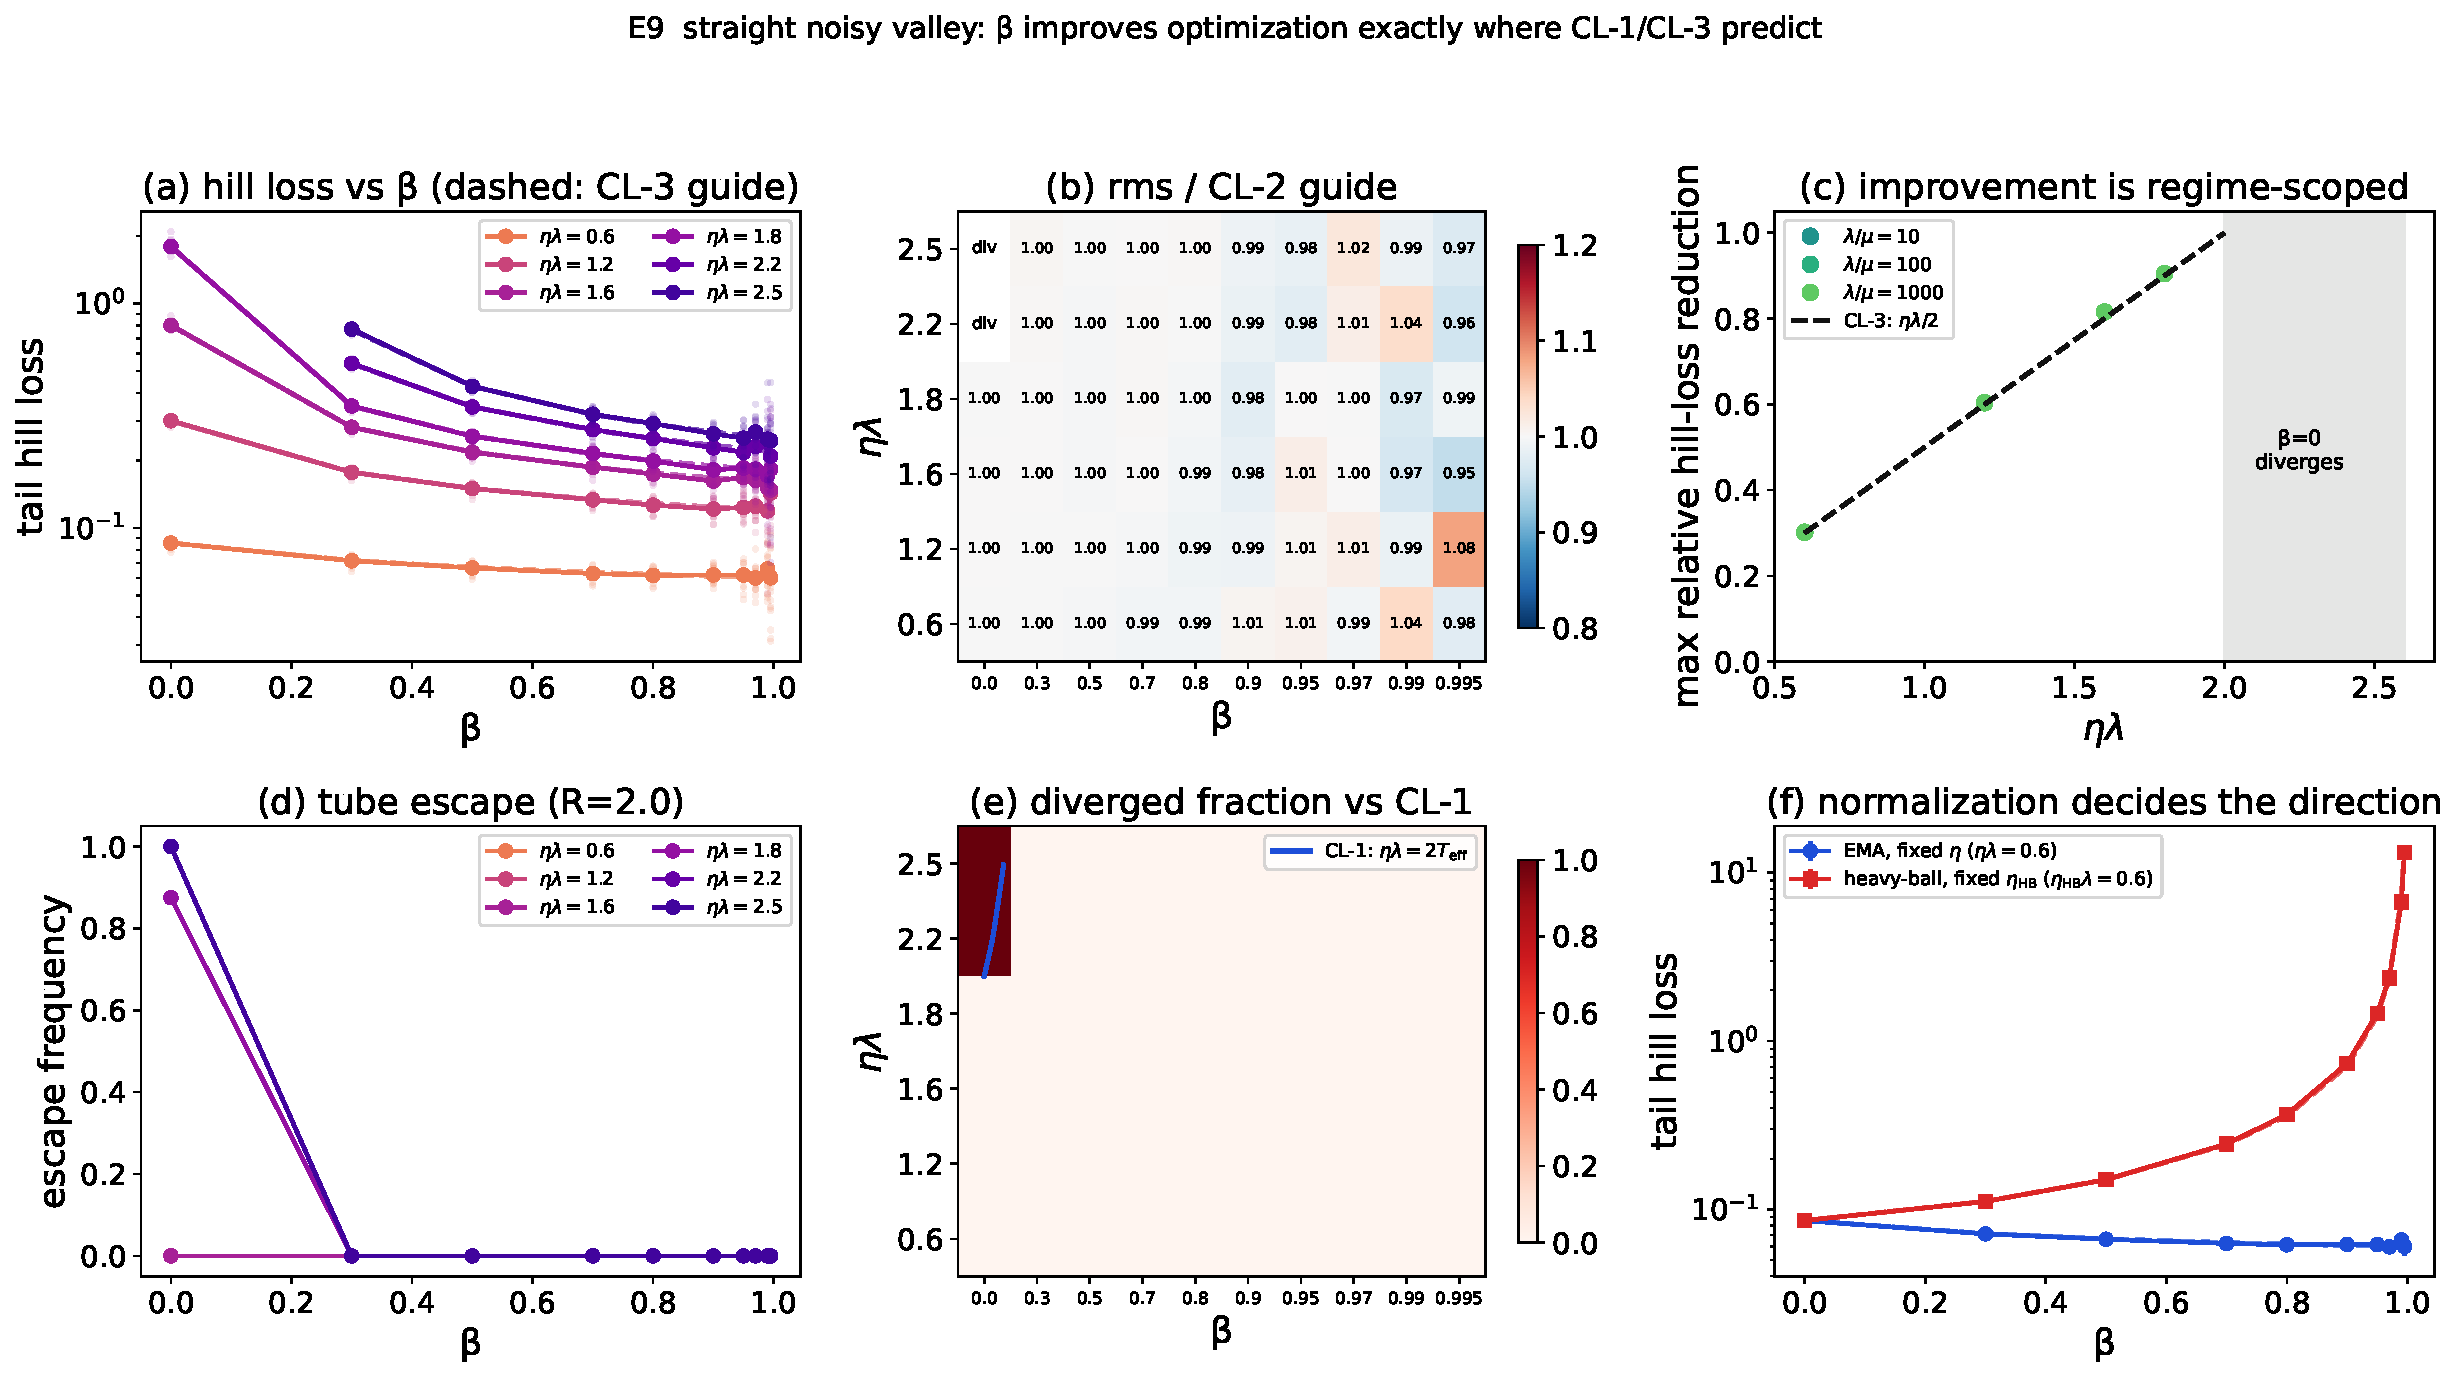
\includegraphics[width=\linewidth]{fig_e9_betaopt}
\caption{Straight noisy valley (E9), $\sigma=2$, $16$ seeds, $T=6000$, tail half scored, $\beta\in\{0,0.3,0.5,0.7,0.8,0.9,0.95,0.97,0.99,0.995\}$.
(a) tail hill loss versus $\beta$ per $\eta\lambda$ at $\lambda/\mu=100$; faint points are per-seed values, dashed the \Cref{cor:hillloss} guide.
(b) measured stationary rms over the \Cref{prop:variance} guide per $(\eta\lambda,\beta)$ cell at $\lambda/\mu=100$; cells beyond the \Cref{prop:stability} threshold marked ``div''.
(c) maximal relative hill-loss reduction per $(\eta\lambda,\lambda/\mu)$, dashed the $\eta\lambda/2$ prediction of \Cref{cor:hillloss}; the shaded band $\eta\lambda\ge2$ is where $\beta=0$ diverges.
(d) tube-escape frequency versus $\beta$ ($R=2$).
(e) diverged-seed fraction per cell with the $\eta\lambda=2\Teff$ boundary of \Cref{prop:stability}.
(f) tail hill loss versus $\beta$ under the EMA convention at fixed $\eta$ ($\eta\lambda=0.6$) and the heavy-ball convention at fixed $\eta_{\mathrm{HB}}$ ($\eta_{\mathrm{HB}}\lambda=0.6$); error bars are seed standard error, dashed the composed guides.
Source: run \texttt{beta\_opt\_sweep\_b10\_el6\_c3\_seeds16}.}
\label{fig:e9}
\end{figure}

\subsection{The $\beta$ window versus bend frequency (E10)}
\label{sec:e10}
The complementary question is why not $\beta\to1$, along the curvature axis of \Cref{rem:window}.
On curved valleys $y=2\sin(kx)$ with the amplitude fixed and the bend wavenumber swept over $k\in\{0.3,0.6,0.9,1.2,1.8\}$ ($k=0.9$ is the E2/E8 landscape; $\lambda/\mu=100$, $\sigma=2$, $16$ seeds, scored over the traveling horizon $3/(\eta\mu)$, tube radius $2.5=1.25\,a_{\mathrm{b}}$ so that escape flags dynamical blow-up rather than marginal corner contact), three things happen as $k$ rises (\Cref{fig:e10}).
First, the confinement floor---the smallest $\beta$ with escape frequency at most $0.25$---rises monotonically: $\beta=0.3$, $0.5$, $0.7$, $0.7$, $0.9$ at $\eta\lambda=1.8$ and $0.3$, $0.5$, $0.7$, $0.8$, $0.95$ at $\eta\lambda=2.5$.
These floors are now predicted: the \Cref{prop:curved} worst-case threshold $\eta\lambda(1+(a_{\mathrm{b}}k)^2)<2\Teff$ reproduces the measured floor exactly in $7$ of the $10$ cells and to one grid step in the other $3$, with misses in both directions---a deterministic stability threshold read against a noise-driven escape criterion.
Second, the $\beta$ window narrows, from six grid steps at $k=0.3$ to four ($\eta\lambda=1.8$) and three ($\eta\lambda=2.5$) at $k=1.8$---the curvature counterpart of the widening with conditioning in \Cref{sec:grid}.
Third, the travel-loss U-shape holds at every $k$: the best $\beta$ is interior and $\beta=0$ escapes at every cell, and at $\eta\lambda=1.8$, $k\ge0.9$ the $\beta=0.999$ arm costs at least $1.5\times$ the best.

One prediction required correction, and the correction is itself a closed-loop statement.
The naive reading of \Cref{rem:tradeoff}---the window's top edge falls as the bend frequency rises---presumes the temporal bend frequency $k\vriv$ is an external dial.
It is not: the measured river speed collapses with $k$ ($\vriv=0.047$ to $0.013$ at $\eta\lambda=1.8$; $0.064$ to $0.015$ at $\eta\lambda=2.5$), so $k\vriv$ self-regulates below the passband edge and the top edge stays soft while the traversal slows.
Curvature is paid in river speed, not only in lag; at $k=1.8$ the $\beta$ window collapses entirely (only the maximal-smoothing $\beta=0.999$ meets the lag criterion, at heavy loss)---beyond this curvature no $\beta$ both filters the hills and follows the river.

\begin{figure}[t]
\centering
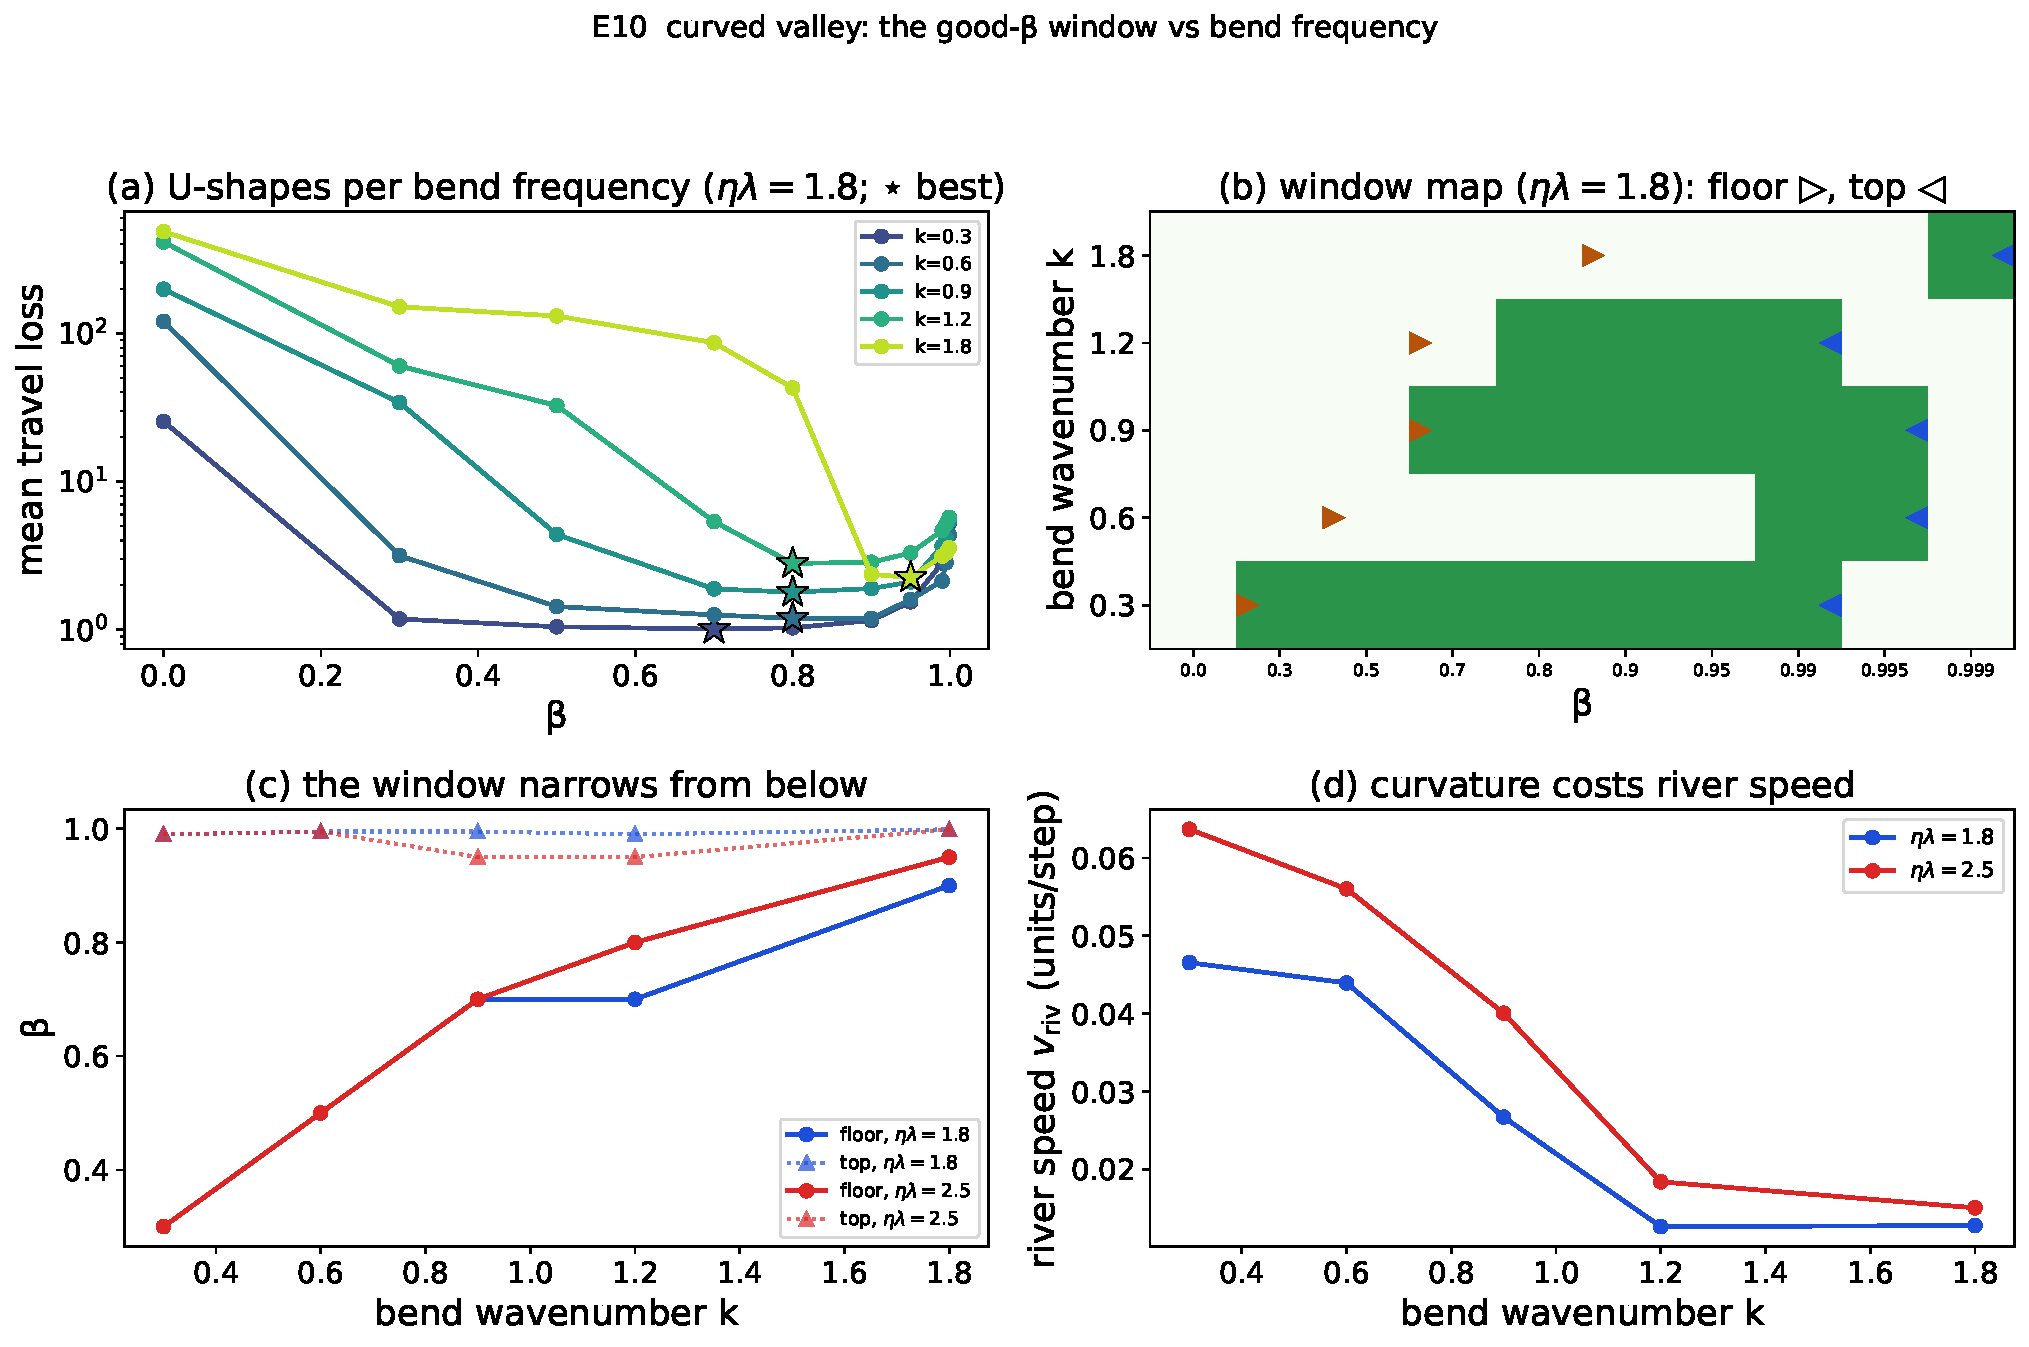
\includegraphics[width=\linewidth]{fig_e10_bendwindow}
\caption{Curved valley versus bend frequency (E10), $f(x)=2\sin(kx)$, $k\in\{0.3,0.6,0.9,1.2,1.8\}$, $\lambda/\mu=100$, $\sigma=2$, $16$ seeds, traveling horizon $3/(\eta\mu)$, tube radius $2.5$.
(a) mean travel loss versus $\beta$ per $k$ at $\eta\lambda=1.8$ (log), stars at the best $\beta$.
(b) window map at $\eta\lambda=1.8$: filled cells satisfy escape $\le0.25$ and lag $\le1.25\times$ the row minimum (contiguous around the lag minimum); markers give the confinement floor ($\rhd$) and the lag-criterion top ($\lhd$).
(c) floor and top edges versus $k$ for $\eta\lambda\in\{1.8,2.5\}$.
(d) measured river speed $\vriv$ versus $k$.
Source: run \texttt{bend\_window\_sweep\_k5\_el2\_b10\_seeds16}.}
\label{fig:e10}
\end{figure}

\subsection{Forced-disturbance controls (E13)}
\label{sec:e13}
If filtering is the mechanism, the outcome must follow the disturbance's frequency content, not $\beta$.
On the straight noisy valley ($\eta\lambda=1.8$, $\sigma=1$), a deterministic tone $A\cos(\omega t)$ with $A=3$ is added to the hill gradient and swept over four frequencies at $\beta\in\{0,\dots,0.99\}$ ($T=6000$, tail half scored, $12$ seeds; \Cref{fig:e13}).
Every $(\omega,\beta)$ cell carries the parameter-free \Cref{prop:forced} guide, and the measured tail hill loss sits on it in $28$ of $28$ cells (within twice the seed standard error plus $5\%$), across nearly three orders of magnitude ($0.044$ to $36.6$).

At $\omega=\pi$, momentum removes the tone: the forced-amplitude ratio between $\beta=0.99$ and $\beta=0$ is $5.03\times10^{-4}$ (guide $5.05\times10^{-4}$), and the $\beta=0$ tail hill loss of $36.6$---the tone amplified by the near-critical loop---falls to $0.044$ at $\beta=0.95$.
At $\omega=0.02$, in the passband, no $\beta$ removes it: the forced amplitude is flat in $\beta$ (max/min $1.022$ over the grid, guide $1.02$), the $\beta$-free displacement of \Cref{prop:forced}(a).
At $\omega=\theta_{0.9}=0.436$, the $\beta=0.9$ hill-mode frequency, momentum \emph{hurts}: tail hill loss $4.14$ at $\beta=0.9$ against $0.69$ at $\beta=0$, a factor $6.0$ (guide $6.0$)---and the harm is frequency-matched, since the same tone costs $\beta=0.99$ only $0.047$ (its resonance sits elsewhere).
Performance tracks the frequency content through the gain curve, not the momentum coefficient.

\begin{figure}[t]
\centering
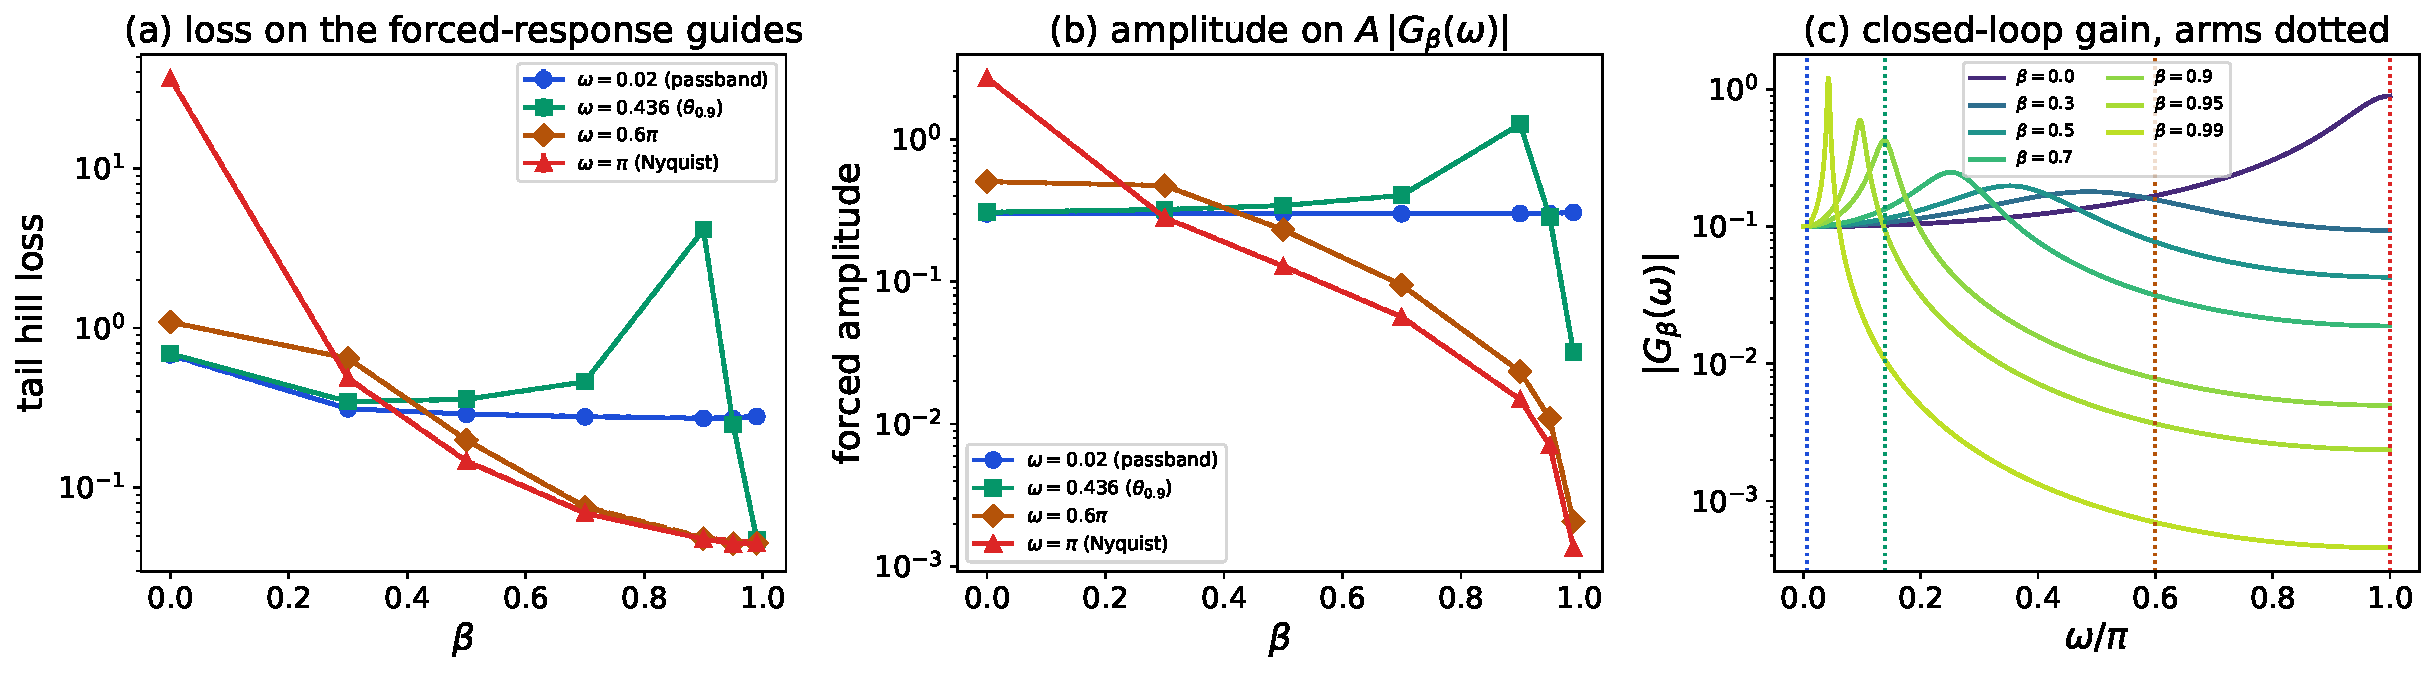
\includegraphics[width=\linewidth]{fig_e13_forced}
\caption{Forced-disturbance controls (E13), straight noisy valley, $\eta\lambda=1.8$, $\sigma=1$, tone amplitude $A=3$ on the hill gradient, $T=6000$, tail half scored, $12$ seeds.
(a) tail hill loss versus $\beta$ per forcing frequency $\omega\in\{0.02,\theta_{0.9}{=}0.436,0.6\pi,\pi\}$ (log); dashed the \Cref{prop:forced} guides; error bars are seed standard error.
(b) forced amplitude versus $\beta$ per $\omega$ (log), dashed the $A\lvert G_\beta(\omega)\rvert$ guides.
(c) gain $\lvert G_\beta(\omega)\rvert$ versus $\omega$ per $\beta$ (log), with the four forcing frequencies marked.
Source: run \texttt{forced\_controls\_sweep\_om4\_b7\_seeds12}.}
\label{fig:e13}
\end{figure}

\subsection{Straight valley (E1)}
\label{sec:e1}
With $\mu=0.1$, $\lambda=10$, $\eta=0.18$ (so $\eta\lambda=1.8$), the hill gradient changes sign $72$ times at $\beta=0$.
\Cref{fig:e1} and \Cref{tab:e1} report the outcome.
On the gradient stream the buffer follows the filter bound of \Cref{thm:filter}: the hill suppression ratio decreases monotonically in $\beta$, the high-band momentum suppression ratio tracks $\Hmag{\pi}^2$, and the momentum river alignment exceeds the raw-gradient alignment for every $\beta>0$.
The closed-loop trajectory follows \Cref{rem:closedloop} instead: the rms distance to the floor is smallest at $\beta=0.5$ and grows for $\beta\ge0.9$, worst at $\beta=0.99$, where the underdamped hill mode rings across the whole window.
The open-loop attenuation and the closed-loop floor distance are optimized at different $\beta$, so filter attenuation alone does not predict the trajectory.

\begin{figure}[t]
\centering
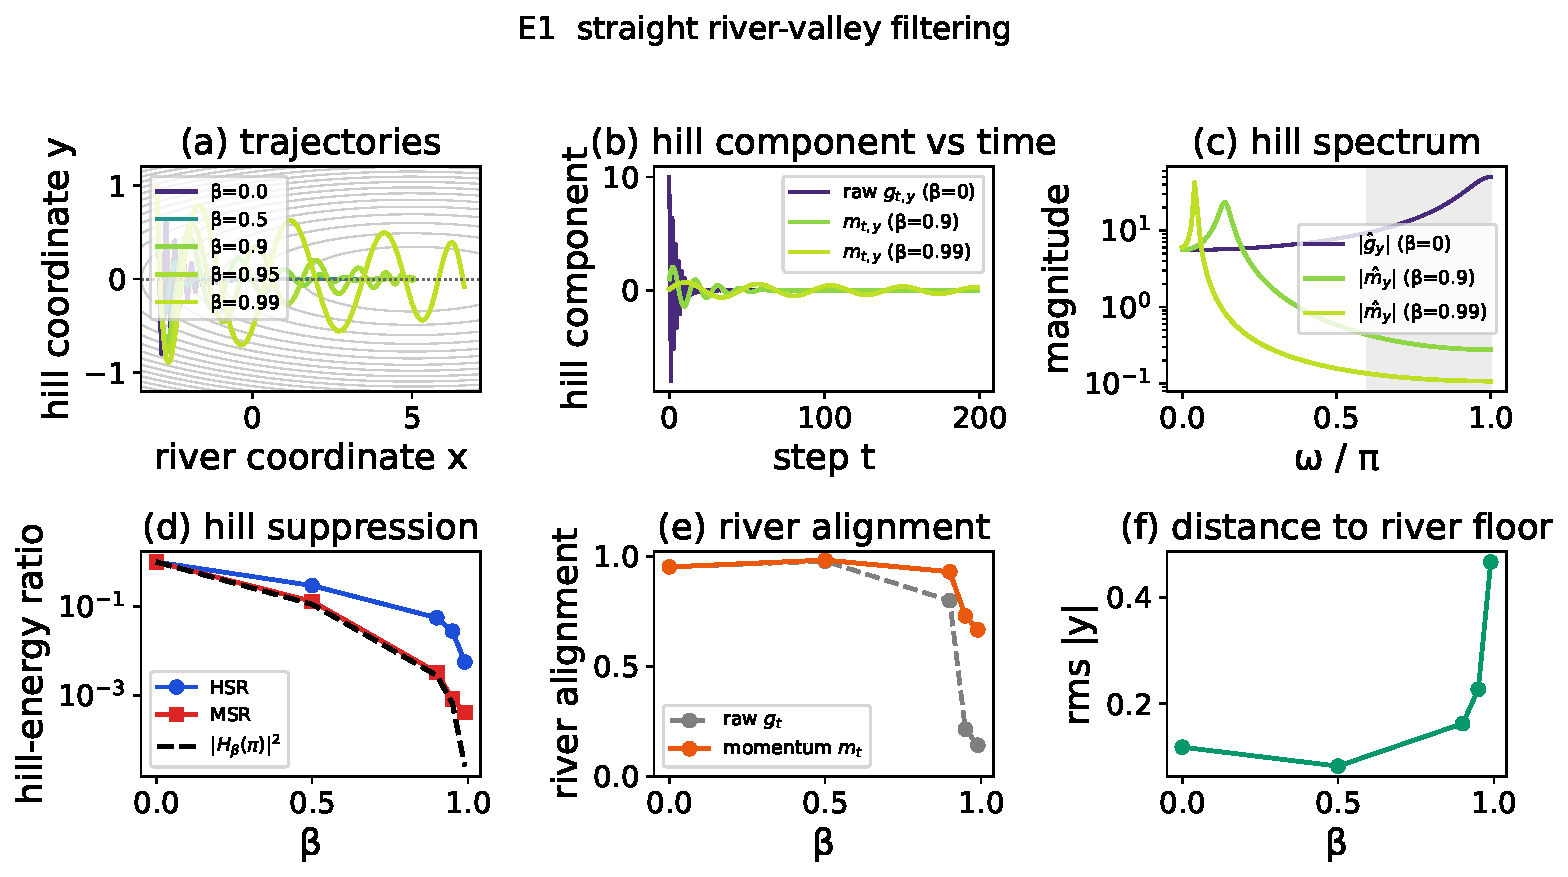
\includegraphics[width=\linewidth]{fig_e1_straight}
\caption{Straight river valley (E1), $\beta\in\{0,0.5,0.9,0.95,0.99\}$, $\eta\lambda=1.8$, $T=200$.
(a) iterate trajectories on the loss contour.
(b) hill component over time: raw $g_{t,y}$ at $\beta=0$ and momentum $m_{t,y}$ at $\beta\in\{0.9,0.99\}$.
(c) temporal spectrum of the hill component (rectangular window), high band $\omega\ge0.6\pi$ shaded.
(d) hill suppression ratio HSR and momentum suppression ratio MSR versus $\beta$ with the $\Hmag{\pi}^2$ guide.
(e) per-step river alignment of $g_t$ and $m_t$, averaged over $t$.
(f) rms distance to the river floor.
Source: run \texttt{straight\_valley\_trajectory\_eta0p18\_lam10\_T200}.}
\label{fig:e1}
\end{figure}

\begin{table}[t]
\centering
\caption{Straight valley (E1) by momentum coefficient.
HSR, MSR, river alignment of the raw gradient $\Align_\Rcal(g)$ and of momentum $\Align_\Rcal(m)$, and rms floor distance $d_{\mathrm{rms}}$, against the Nyquist guide $\Hmag{\pi}^2$.
Values from \texttt{metrics.json}.}
\label{tab:e1}
\begin{tabular}{lcccccc}
\toprule
$\beta$ & HSR & MSR & $\Hmag{\pi}^2$ & $\Align_\Rcal(g)$ & $\Align_\Rcal(m)$ & $d_{\mathrm{rms}}$\\
\midrule
$0$    & $1.00$  & $1.00$   & $1.00$   & $0.951$ & $0.951$ & $0.118$\\
$0.5$  & $0.294$ & $0.130$  & $0.111$  & $0.978$ & $0.982$ & $0.082$\\
$0.9$  & $0.0554$& $0.00327$& $0.00277$& $0.798$ & $0.929$ & $0.162$\\
$0.95$ & $0.0277$& $0.000821$&$0.000657$&$0.214$ & $0.729$ & $0.226$\\
$0.99$ & $0.00558$&$0.000410$&$0.0000253$&$0.141$&$0.665$ & $0.466$\\
\bottomrule
\end{tabular}
\end{table}

\subsection{Curved valley (E2)}
\label{sec:e2}
With floor $f(x)=2\sin(0.9x)$ and $\eta\lambda=1.8$, river alignment to the live tangent rises from $0.136$ at $\beta=0$ to $0.991$ at $\beta=0.9$, then falls to $0.935$ at $\beta=0.99$ (\Cref{fig:e2}).
The hill-normal energy of the buffer falls by about six orders of magnitude from $\beta=0$ to $\beta=0.9$, and the river-following lag is smallest at $\beta=0.9$ and grows again at $\beta=0.99$: larger $\beta$ removes hill energy but a too-large $\beta$ lags the bend.
The optimum at moderate $\beta$ is the filtering--lag tradeoff of \Cref{rem:tradeoff}.

\begin{figure}[t]
\centering
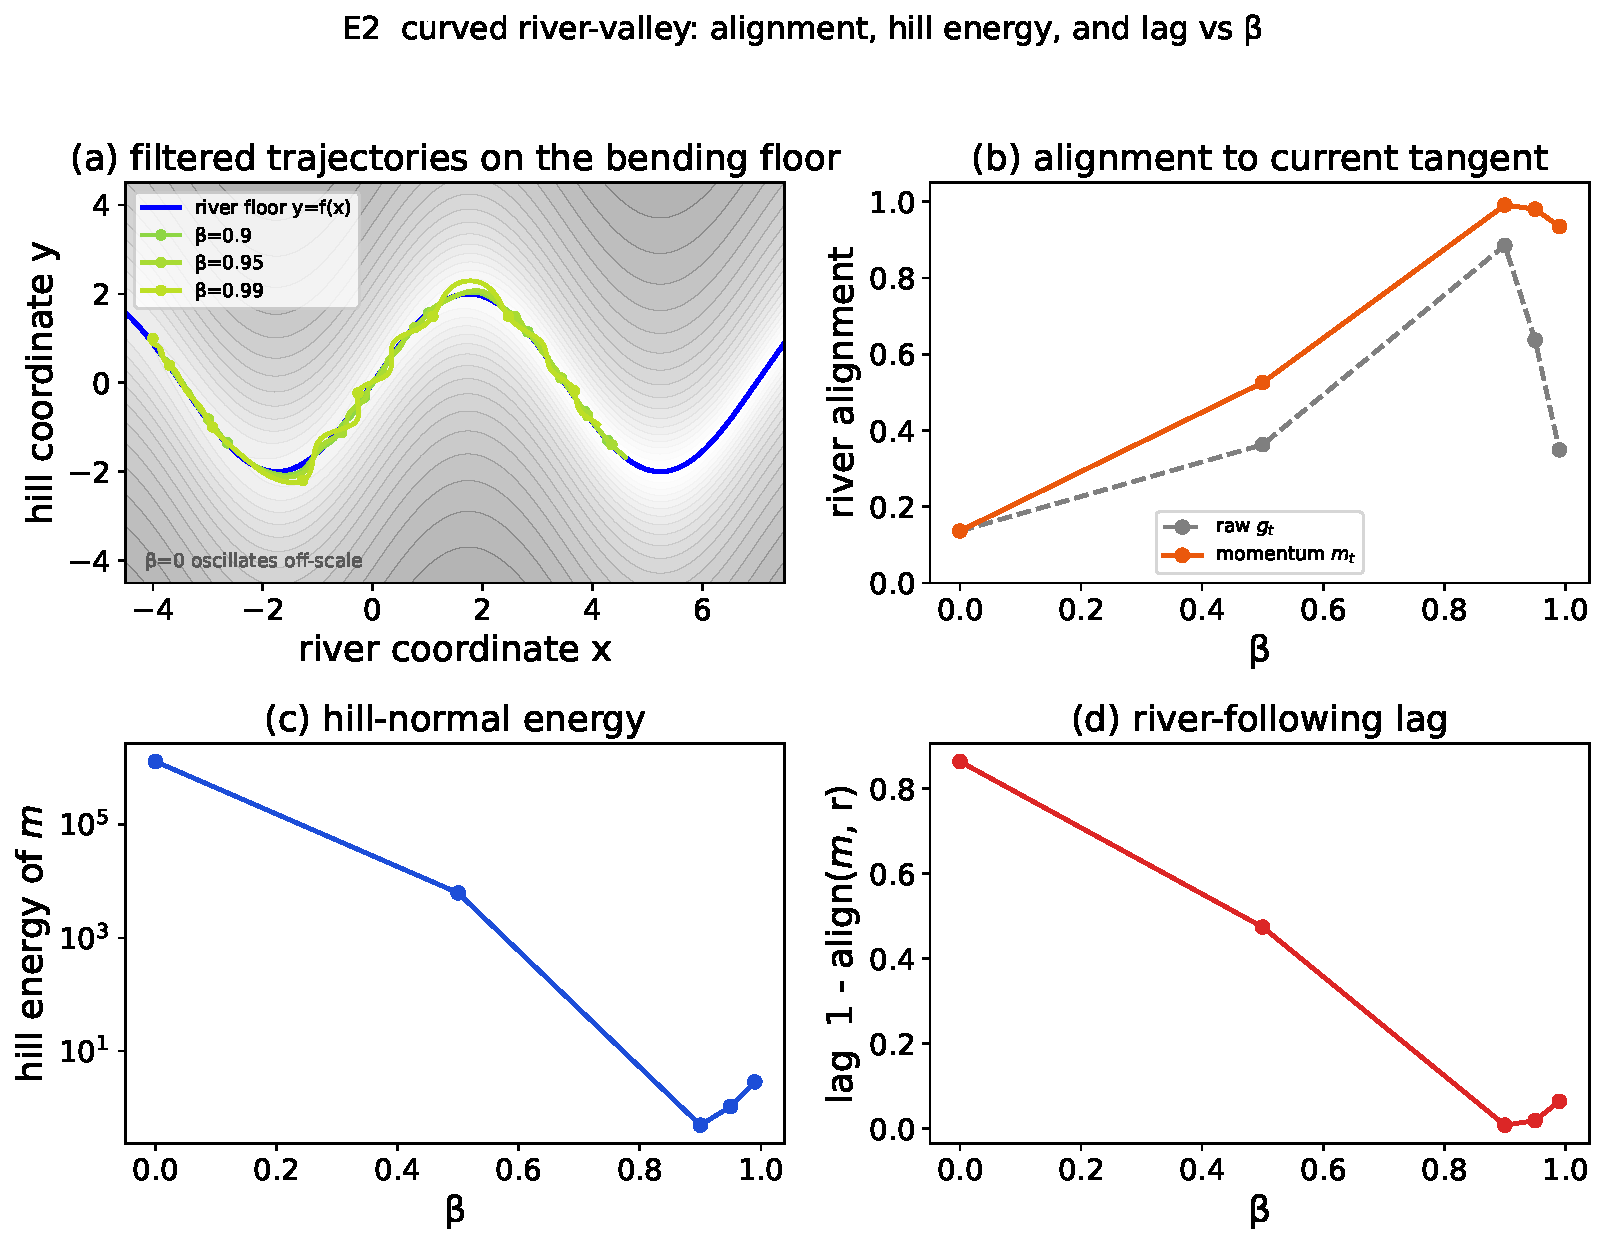
\includegraphics[width=\linewidth]{fig_e2_curved}
\caption{Curved river valley (E2), $f(x)=2\sin(0.9x)$, $\eta\lambda=1.8$, $T=300$.
(a) filtered trajectories ($\beta\in\{0.9,0.95,0.99\}$) on the bending floor; the near-unstable $\beta=0$ baseline is off-scale and quantified in (b)--(d).
(b) river alignment of $g_t$ and $m_t$ versus $\beta$.
(c) hill-normal energy of $m_t$ versus $\beta$ (log).
(d) river-following lag $1-\Align_\Rcal(m_t)$ versus $\beta$.
Source: run \texttt{curved\_valley\_trajectory\_a2\_k0p9\_eta0p18\_T300}.}
\label{fig:e2}
\end{figure}

\subsection{Noise (E3)}
\label{sec:e3}
Adding Gaussian, anisotropic-hill, and heavy-tailed gradient noise to the straight valley over $12$ seeds, the noise suppression ratio---the residual of $m_t$ against the filtered clean gradient---tracks the white-noise floor $1/\Teff$ (Gaussian: $0.330,0.053,0.026,0.0033$ at $\beta=0.5,0.9,0.95,0.99$ against $0.333,0.053,0.026,0.0050$), and momentum raises river alignment over the raw gradient for every $\beta$ and noise model (\Cref{fig:e3}).
Comparing the buffer to the \emph{instantaneous} clean gradient instead yields a non-monotone ratio with a minimum at moderate $\beta$, because that comparison also carries the deterministic lag bias; the two readings separate the variance-reduction effect from the lag.

\begin{figure}[t]
\centering
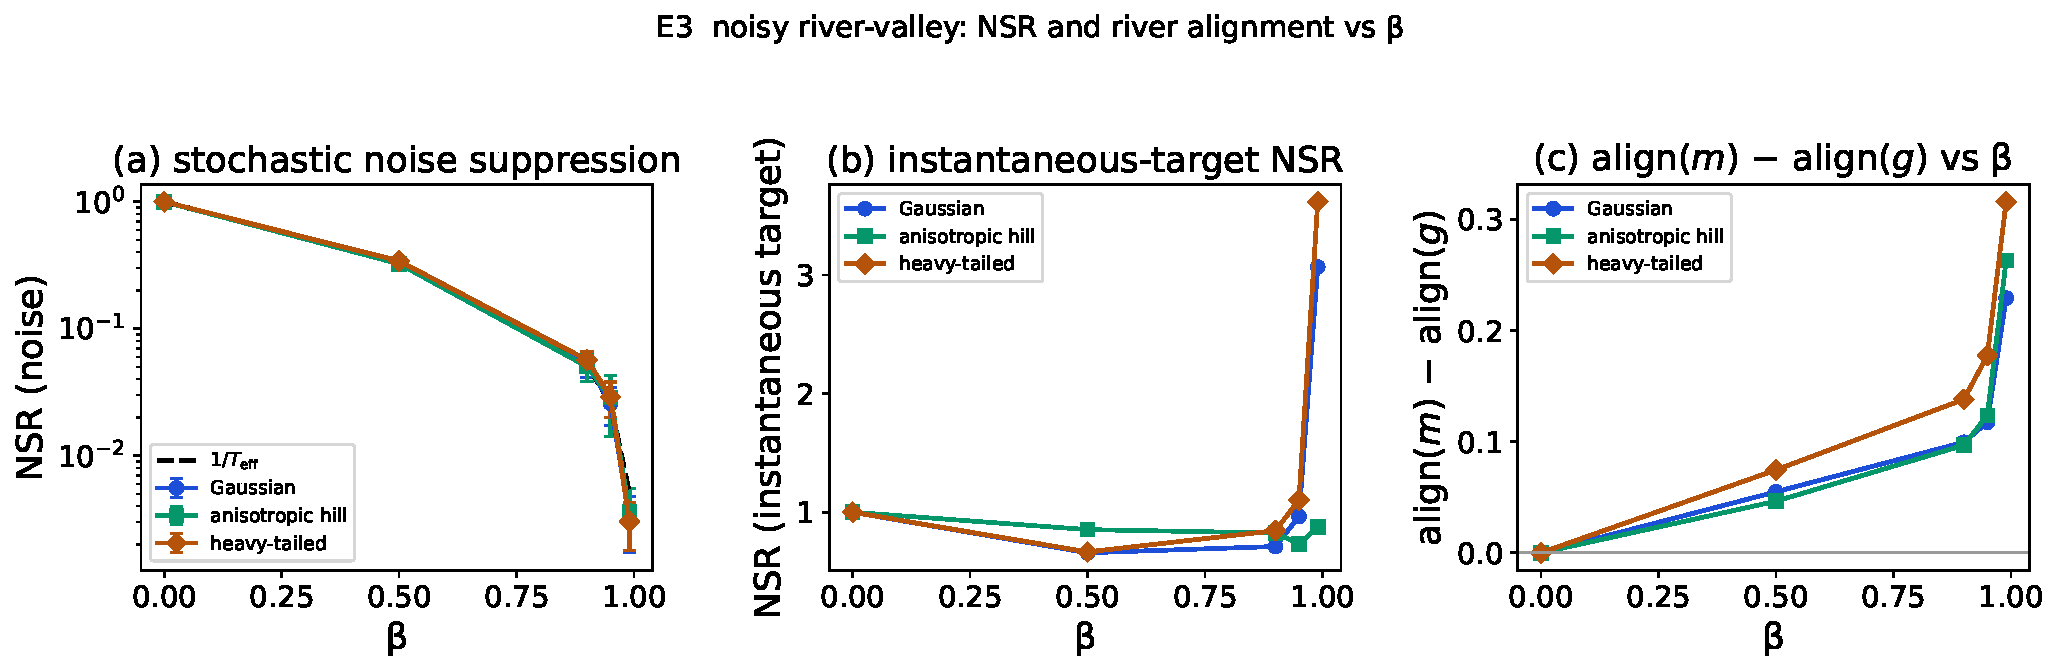
\includegraphics[width=\linewidth]{fig_e3_noise}
\caption{Noisy straight valley (E3), $12$ seeds, $\sigma=2$.
(a) noise suppression ratio NSR versus $\beta$ for three noise models with the $1/\Teff$ floor (log, error bars are seed std).
(b) instantaneous-target ratio versus $\beta$.
(c) river-alignment difference $\Align_\Rcal(m)-\Align_\Rcal(g)$ versus $\beta$.
Source: run \texttt{noisy\_valley\_trajectory\_sig2p0\_seeds12\_eta0p18}.}
\label{fig:e3}
\end{figure}

\subsection{Frequency-domain validation (E4)}
\label{sec:e4}
On fixed gradient streams we form $m=\mathrm{EMA}_\beta(g)$ and compare the empirical per-bin ratio $\lvert\hat m(\omega)\rvert/\lvert\hat g(\omega)\rvert$ with $\Hmag{\omega}$ (\Cref{fig:e4}).
The weighted-median relative error on significant bins is below $0.001$ for a synthetic slow-plus-fast stream, below $0.003$ for a curved-valley hill stream, and at most $0.115$ for a straight-valley hill stream, where the early oscillation transient sits at the window boundary (\Cref{prop:transfer}).
The high-band median ratios sit within $6\%$ of the Nyquist floor $(1-\beta)/(1+\beta)$ for the synthetic and curved streams and within $12\%$ for the boundary-affected straight stream.
The straight-valley hill stream has no low-frequency energy, as \Cref{thm:separation} predicts.

\begin{figure}[t]
\centering
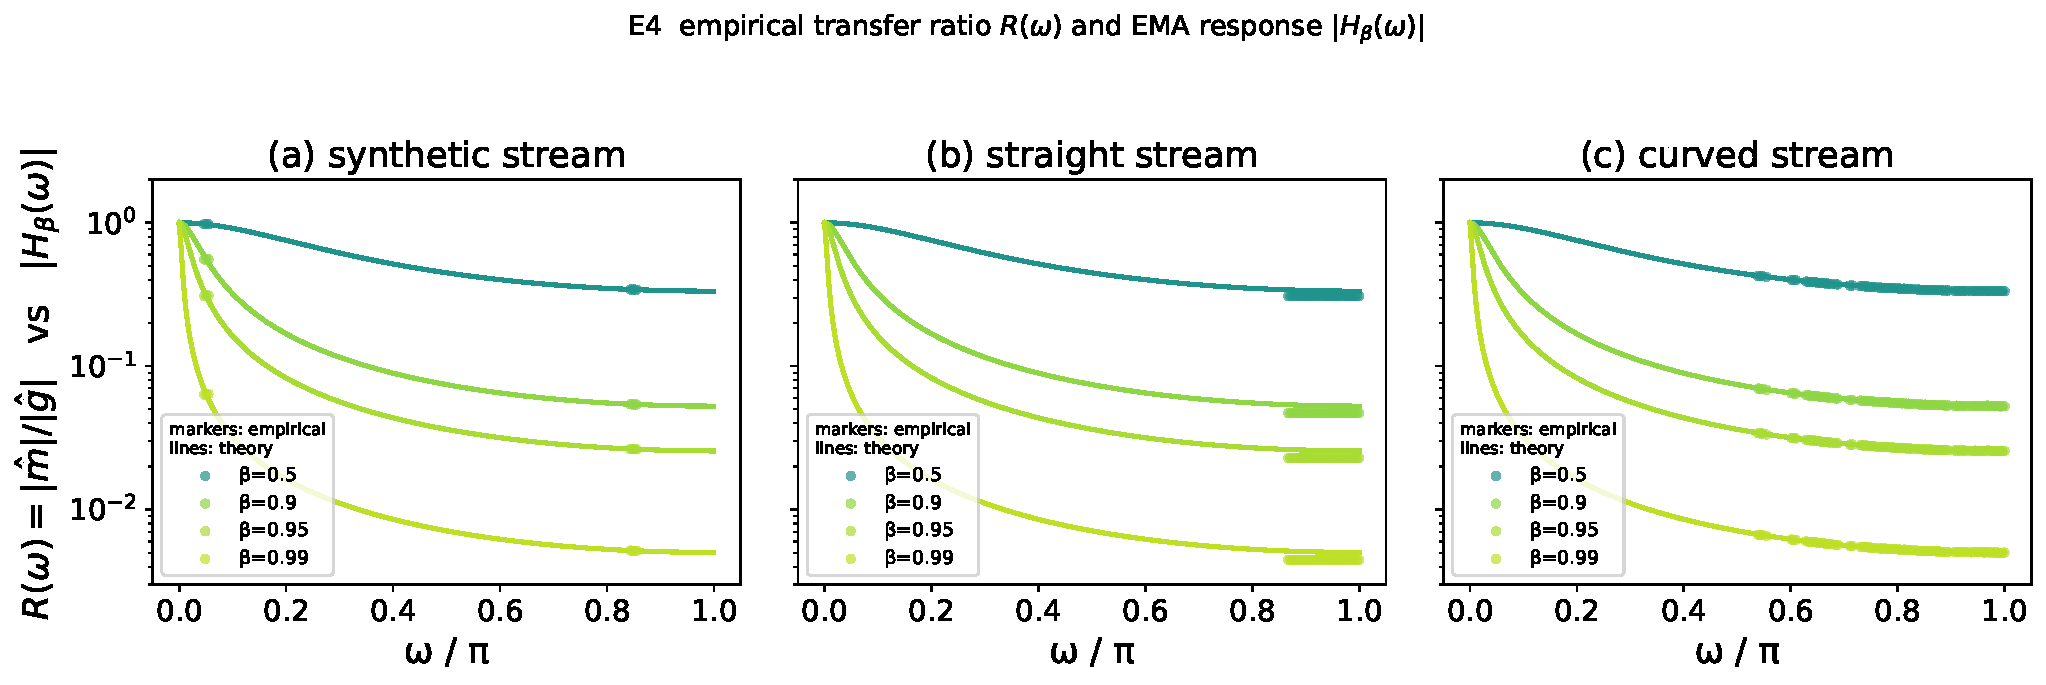
\includegraphics[width=\linewidth]{fig_e4_frequency}
\caption{Empirical EMA transfer ratio versus theory (E4), $T=512$, Hann window.
Each panel is a fixed input stream (synthetic, straight-valley hill, curved-valley hill); markers are the measured ratio $\lvert\hat m\rvert/\lvert\hat g\rvert$ on significant-energy bins, solid lines are $\Hmag{\omega}$, for $\beta\in\{0.5,0.9,0.95,0.99\}$ (log).
Source: run \texttt{frequency\_validation\_spectral\_T512\_hann}.}
\label{fig:e4}
\end{figure}

\subsection{Matrix / Muon toy (E5)}
\label{sec:matrix}
We build $\Gbf_t=\Sbf_t+(-1)^t\Abf+\Xibf_t$ with a slowly varying rank-$3$ signal $\Sbf_t$, a deterministic high-frequency hill $(-1)^t\Abf$, and Gaussian $\Xibf_t$, and compare pre-polar $\polar(\mathrm{EMA}(\Gbf))$, post-polar $\mathrm{EMA}(\polar(\Gbf))$, and polar-only $\polar(\Gbf)$ (\Cref{tab:e5}, \Cref{fig:e5}).
Pre-polar attains the smallest principal-angle error to the signal subspace and the highest signal alignment in \emph{both} the deterministic high-frequency scenario and a stochastic control.
This is the empirical face of \Cref{thm:filterfirst}, with the polar-only column the generic form of \Cref{prop:polaronly}.
Post-polar improves the subspace but loses magnitude (its alignment falls at large $\beta$ as it averages rotated orthogonal factors, the floor of \Cref{rem:postpolar}), so the magnitude-free subspace error is the fair comparison.

A noise-free replica of the high-frequency scenario overlays the constants of \Cref{thm:filterfirst} on the measured traces (\Cref{fig:e5wedin}).
The buffer tail $\sigma_{r+1}(\Mbf_t)$ sits inside the two-sided $\lvert\varepsilon_t\rvert$ envelope at every step, with the upper guide tight to a median factor $1.05$ over the second half; the measured subspace error stays below the bound of \Cref{thm:filterfirst}(b) wherever its gap condition holds, with end-of-run ratio $1.17$ at $\beta=0.9$ and $1.16$ at $\beta=0.99$.
In the noisy scenario the deterministic guide alone under-predicts the tail at large $\beta$---the stochastic floor of \citet{li2026denoise} dominates there---and the guide plus an iid-Gaussian operator-norm floor tracks the measured level.

\begin{figure}[t]
\centering
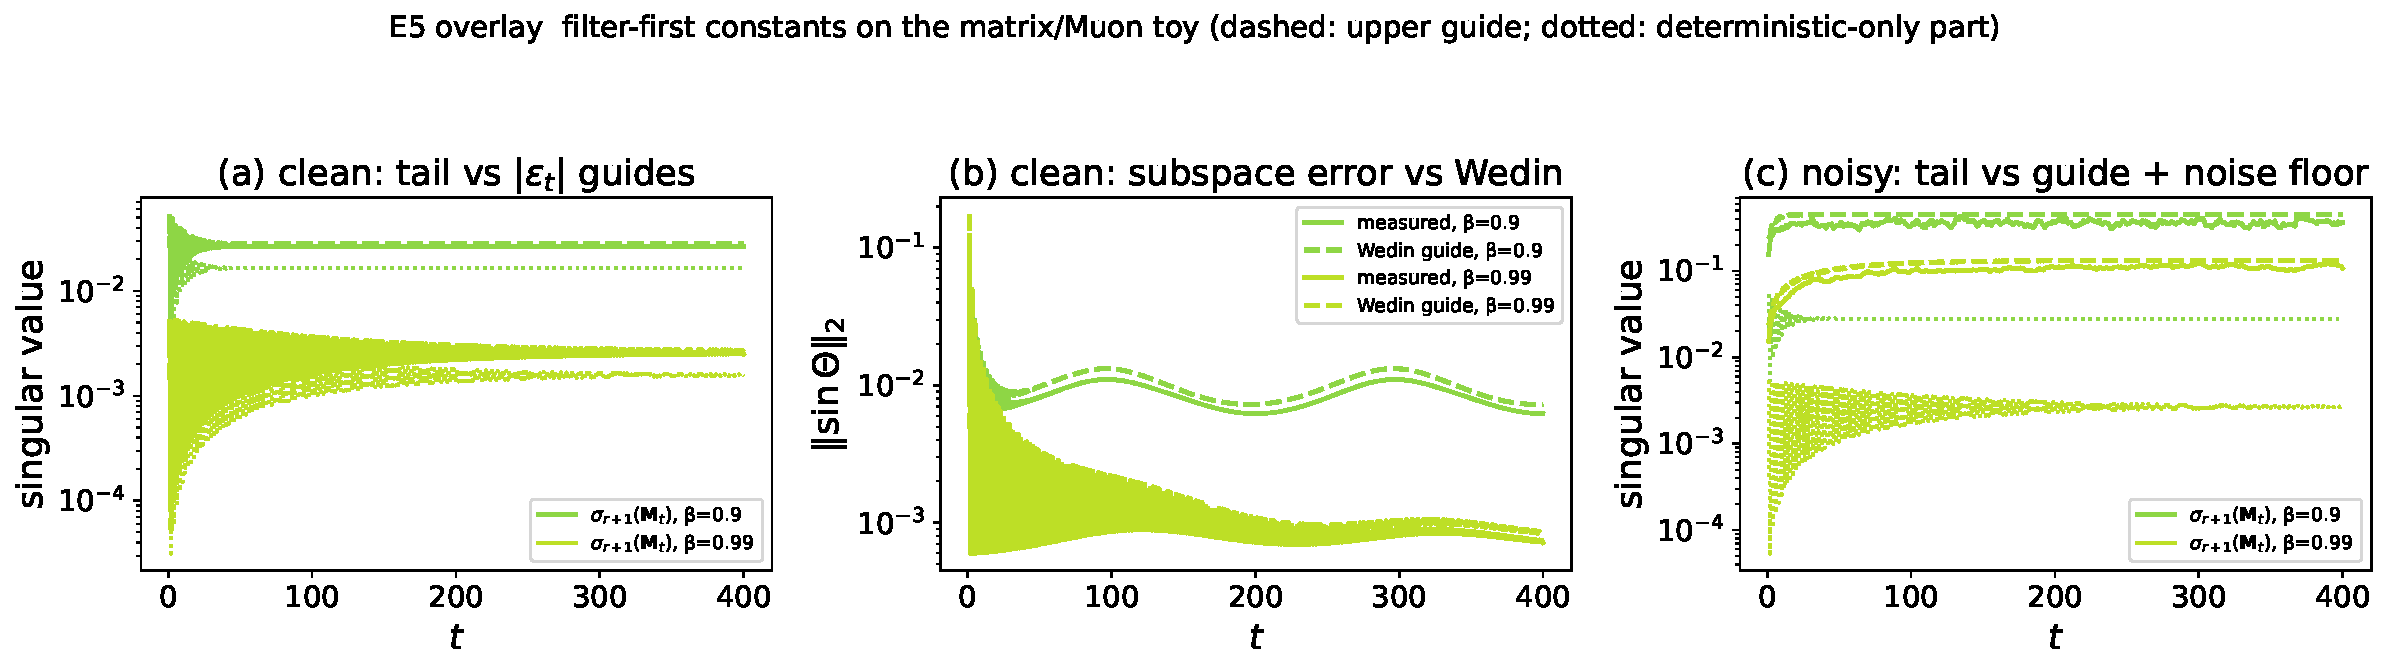
\includegraphics[width=\linewidth]{fig_e5_wedin}
\caption{Constants of \Cref{thm:filterfirst} on the matrix/Muon toy (E5 overlay), $d_1{=}24,d_2{=}18,r{=}3$, $T=400$, $\beta\in\{0.9,0.99\}$.
(a) noise-free scenario: measured $\sigma_{r+1}(\Mbf_t)$ (solid) against the upper guide $\lvert\varepsilon_t\rvert\lVert\Abf\rVert_2$ (dashed) and lower guide $\lvert\varepsilon_t\rvert\sigma_{2r+1}(\Abf)$ (dotted), log scale.
(b) noise-free scenario: measured subspace error (solid) against the bound of \Cref{thm:filterfirst}(b) (dashed).
(c) noisy scenario ($\sigma_\xi=0.2$): measured tail against the deterministic guide (dotted) and the guide plus the iid-Gaussian operator-norm floor (dashed).
Source: run \texttt{matrix\_muon\_pipeline\_m24n18r3\_T400}.}
\label{fig:e5wedin}
\end{figure}

\begin{table}[t]
\centering
\caption{Matrix/Muon toy (E5): subspace error $\lVert\sin\Theta\rVert_2$ (lower better) at $\beta=0.9$, by pipeline and disturbance type.
Values from \texttt{metrics.json}.}
\label{tab:e5}
\begin{tabular}{lccc}
\toprule
disturbance & pre-polar & post-polar & polar-only\\
\midrule
high-frequency $(-1)^t\Abf$ & $0.114$ & $0.133$ & $0.508$\\
stochastic $\Xibf_t$           & $0.171$ & $0.199$ & $0.698$\\
\bottomrule
\end{tabular}
\end{table}

\begin{figure}[t]
\centering
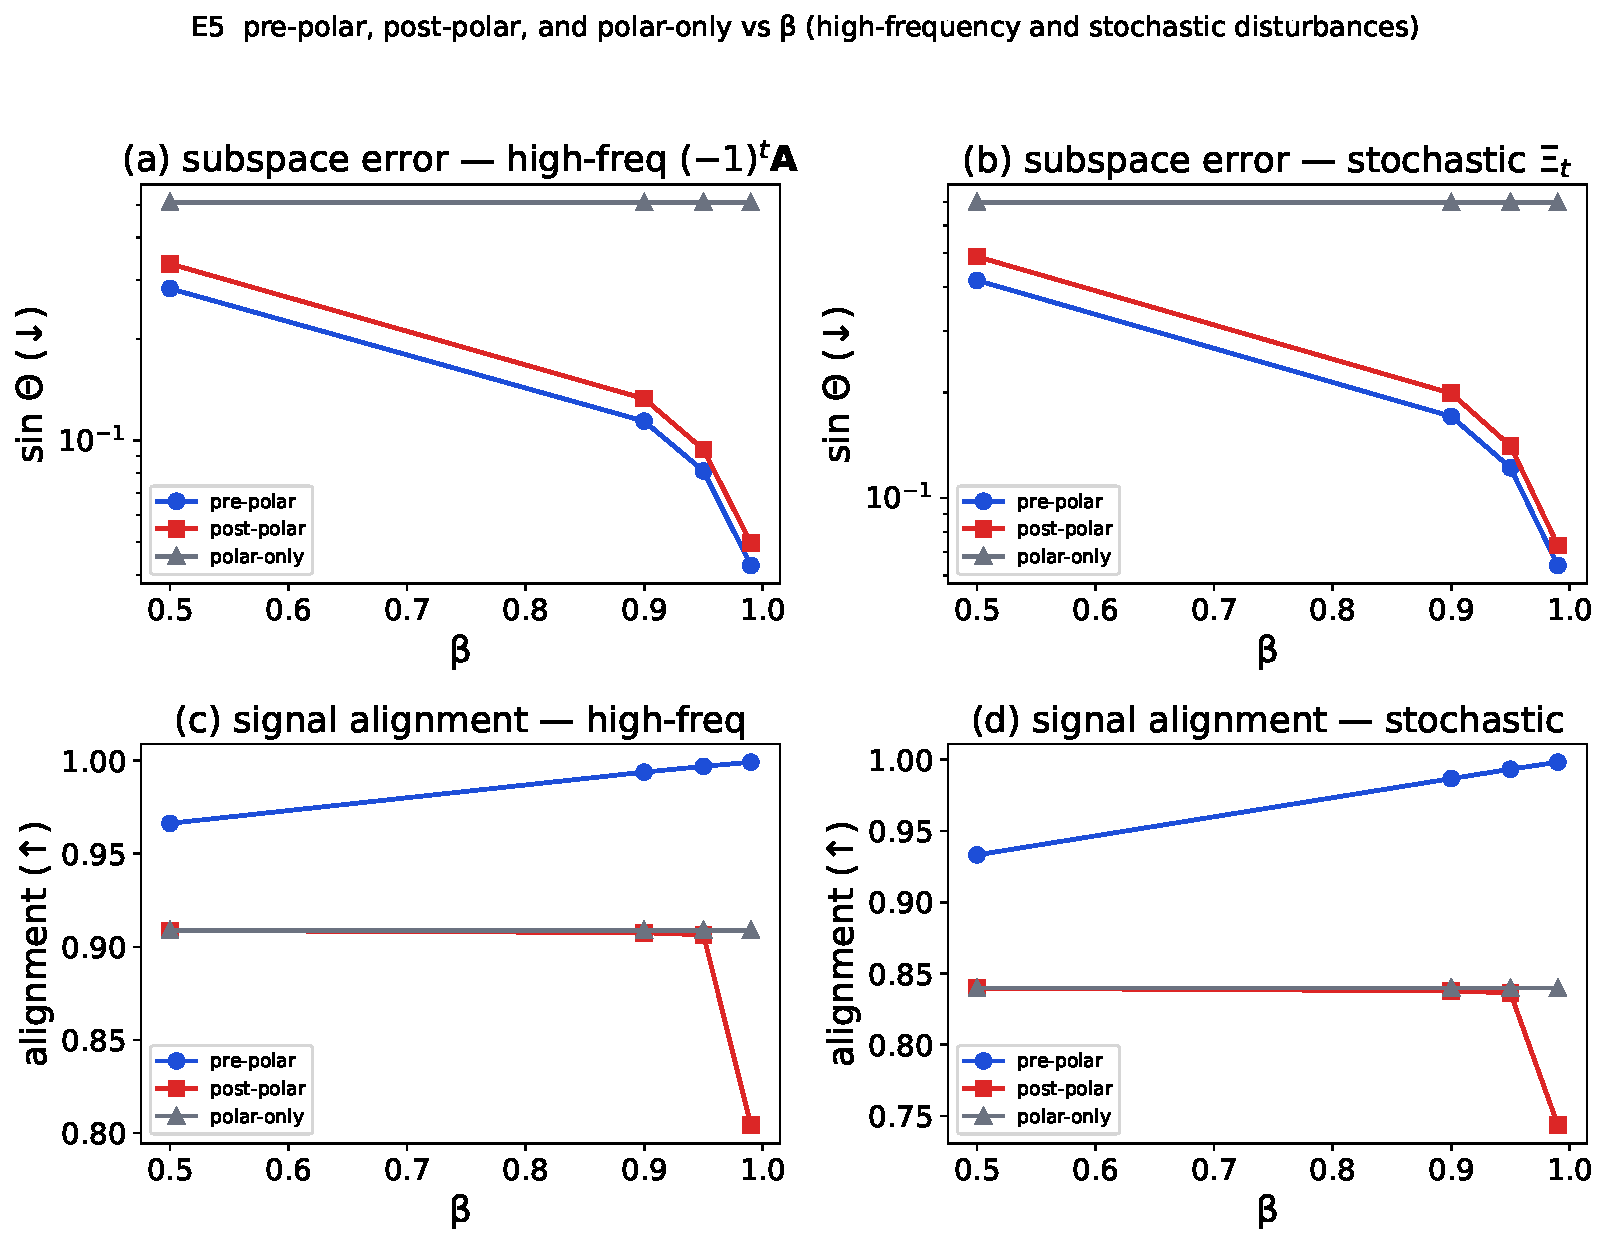
\includegraphics[width=\linewidth]{fig_e5_matrix}
\caption{Filter-first on the matrix/Muon toy (E5), $d_1{=}24,d_2{=}18,r{=}3$, $T=400$.
Subspace error $\lVert\sin\Theta\rVert_2$ (log, lower better) versus $\beta$ for (a) the high-frequency disturbance and (b) the stochastic disturbance; rank-$r$ signal alignment (higher better) versus $\beta$ for (c) high-frequency and (d) stochastic.
Series: pre-polar, post-polar, polar-only.
Source: run \texttt{matrix\_muon\_pipeline\_m24n18r3\_T400}.}
\label{fig:e5}
\end{figure}

\subsection{Regimes of the closed loop (E8)}
\label{sec:e8}
The closed-loop propositions predict a regime map, drawn as trajectory families on the curved valley of E2 with the Gaussian noise of E3 ($\sigma=2$, $12$ seeds, $T=300$; \Cref{fig:e8}).
At $\eta\lambda=1.8$ (panel a), $\beta=0$ escapes the tube on every seed (tail rms $4.25$ against a tube radius $R=2$): the local hill sharpness on a bend is $\lambda(1+f'(x)^2)$ (\Cref{prop:curved}), which exceeds the $\beta=0$ threshold wherever $\lvert f'\rvert>\sqrt{2/(\eta\lambda)-1}$.
At $\beta=0.9$ the trajectory is tube-confined on every seed and its tail rms matches \Cref{prop:variance}: measured $0.194$ against the guide $0.194$.
At $\eta\lambda=2.5>2$ (panel b), $\beta=0$ diverges on all $12$ seeds while $\beta=0.9$ tracks the bending river to rms $0.255$ (guide with the \Cref{prop:curved} bend correction $\lambda(1+\mathbb{E}[f'^2])$ in the denominator: $0.249$)---gradient descent cannot run at this learning rate; momentum can, as $\eta\lambda<2\Teff$ requires.
The third $\beta$ closes the map: at $\beta=0.999$ the filter memory outruns the bend, and every metric reverses (tail rms $0.549$ vs $0.194$, tail loss $3.78$ vs $0.65$, final river coordinate $-1.33$ vs $3.68$).
Panel (c) is the deterministic caveat of \Cref{rem:closedloop} in E1's clean straight valley, where $d_{\mathrm{rms}}$ is smallest at moderate $\beta$: without sustained excitation there is nothing for the filter to remove, and the underdamped transient dominates.

\begin{figure}[t]
\centering
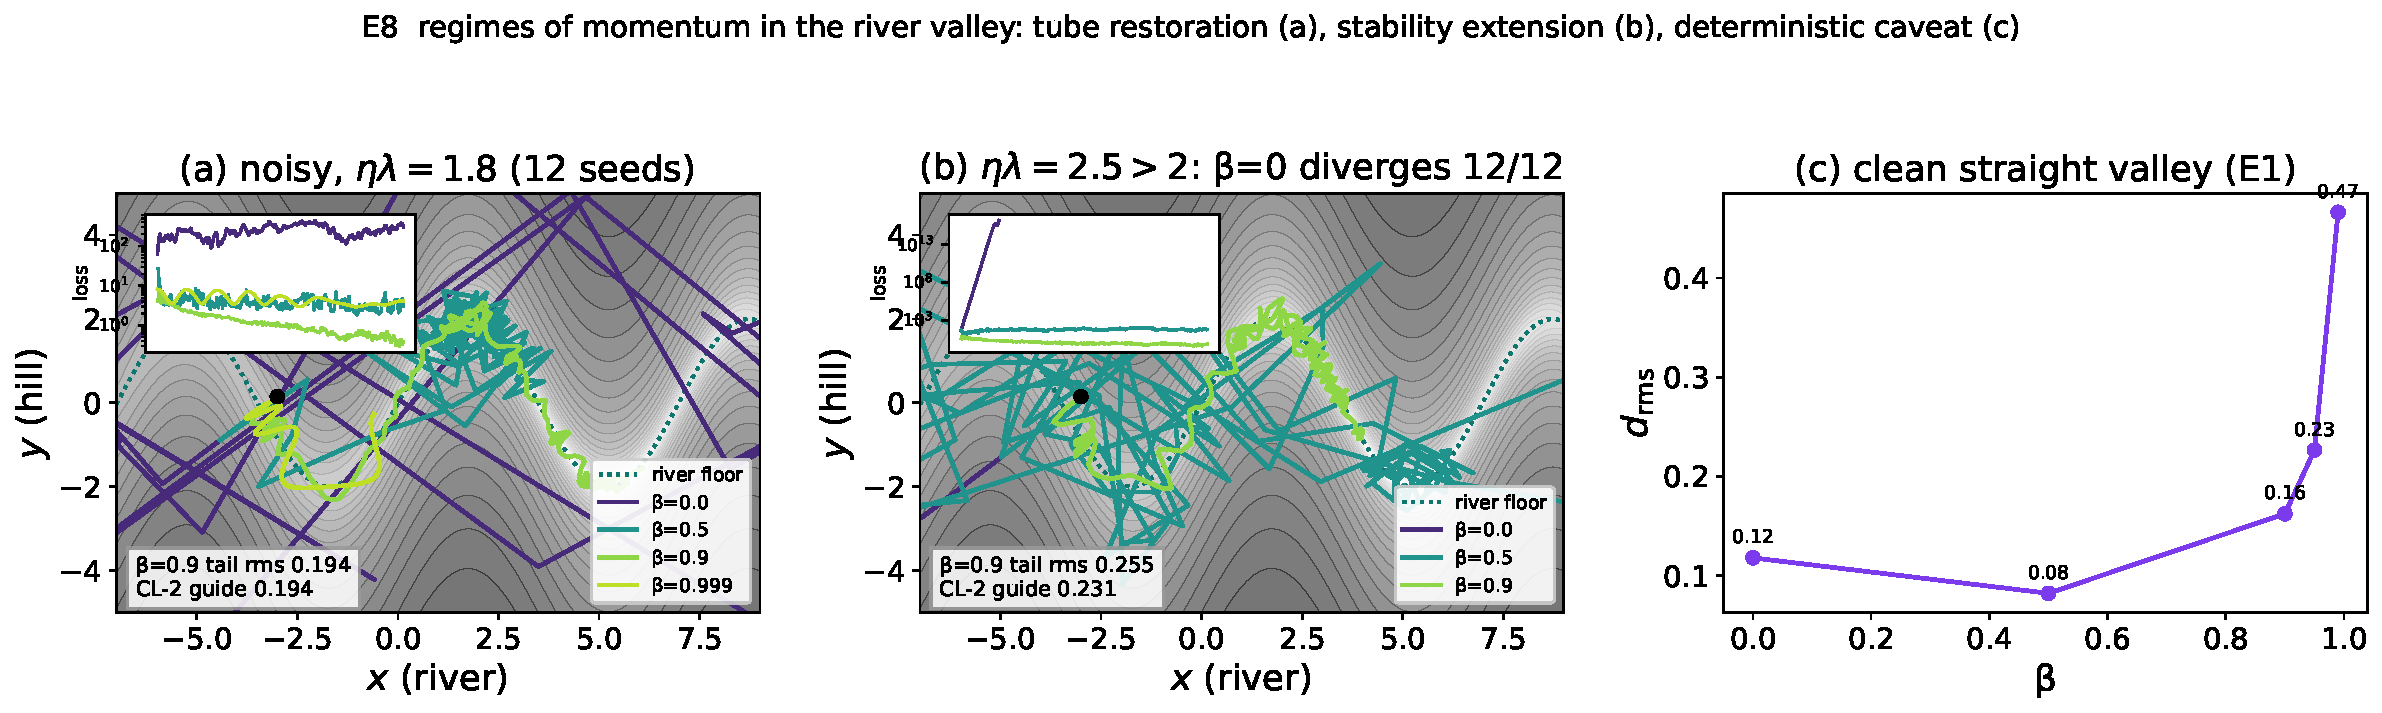
\includegraphics[width=\linewidth]{fig_e8_headline}
\caption{Regimes of momentum in the river valley (E8).
Curved valley $f(x)=2\sin(0.9x)$, Gaussian gradient noise $\sigma=2$, $T=300$, $12$ seeds; trajectories are seed $0$ on the loss contour with the river floor dotted, insets are seed-mean loss (log).
(a) $\eta\lambda=1.8$, $\beta\in\{0,0.5,0.9,0.999\}$; the annotation gives the $\beta=0.9$ seed-mean tail rms of the hill offset against the \Cref{prop:variance} guide.
(b) $\eta\lambda=2.5$, $\beta\in\{0,0.5,0.9\}$; $\beta=0$ diverges on all seeds ($\times$ marks the last finite point).
(c) E1's clean straight valley: $d_{\mathrm{rms}}$ versus $\beta$.
Sources: runs \texttt{valley\_regimes\_trajectory\_eta0p18\_0p25\_sig2\_seeds12\_T300}, \texttt{straight\_valley\_trajectory\_eta0p18\_lam10\_T200}.}
\label{fig:e8}
\end{figure}

\subsection{Stationary variance and the $\beta$ window (closed-loop grid)}
\label{sec:grid}
Three sweeps quantify the closed-loop claims (\Cref{fig:e3heatmap}).
On the straight valley ($8$ seeds, $T=6000$), the measured stationary rms over the grid $\eta\lambda\in\{0.3,\dots,3.0\}\times\beta\in\{0,\dots,0.99\}$ matches the \Cref{prop:variance} guide in $36$ of $37$ comfortably stable cells within twice the seed standard error plus $0.02$, and every cell beyond the \Cref{prop:stability} threshold diverges while none below it does.
On the curved valley, the tube-escape frequency drops from $1$ to $0$ exactly where the predicted rms becomes small against the tube radius---momentum restores the tube-confined regime that river-valley analyses presuppose.
Sweeping the conditioning $\lambda/\mu\in\{10,100,1000\}$ at $\eta\lambda=1.8$, with each conditioning scored over its own traveling horizon $3/(\eta\mu)$, the window of well-performing $\beta$ (no escape, river-following lag within $1.25\times$ its per-conditioning minimum) has upper edge $\beta=0.7$, $0.95$, $0.999$ respectively: the window widens with conditioning, as \Cref{rem:window} predicts, and at $\lambda/\mu=10$ the measured upper edge sits at $\Teff(0.7)=5.7$ against the predicted river-traversal scale $1/(\eta\mu)=5.6$.

\begin{figure}[t]
\centering
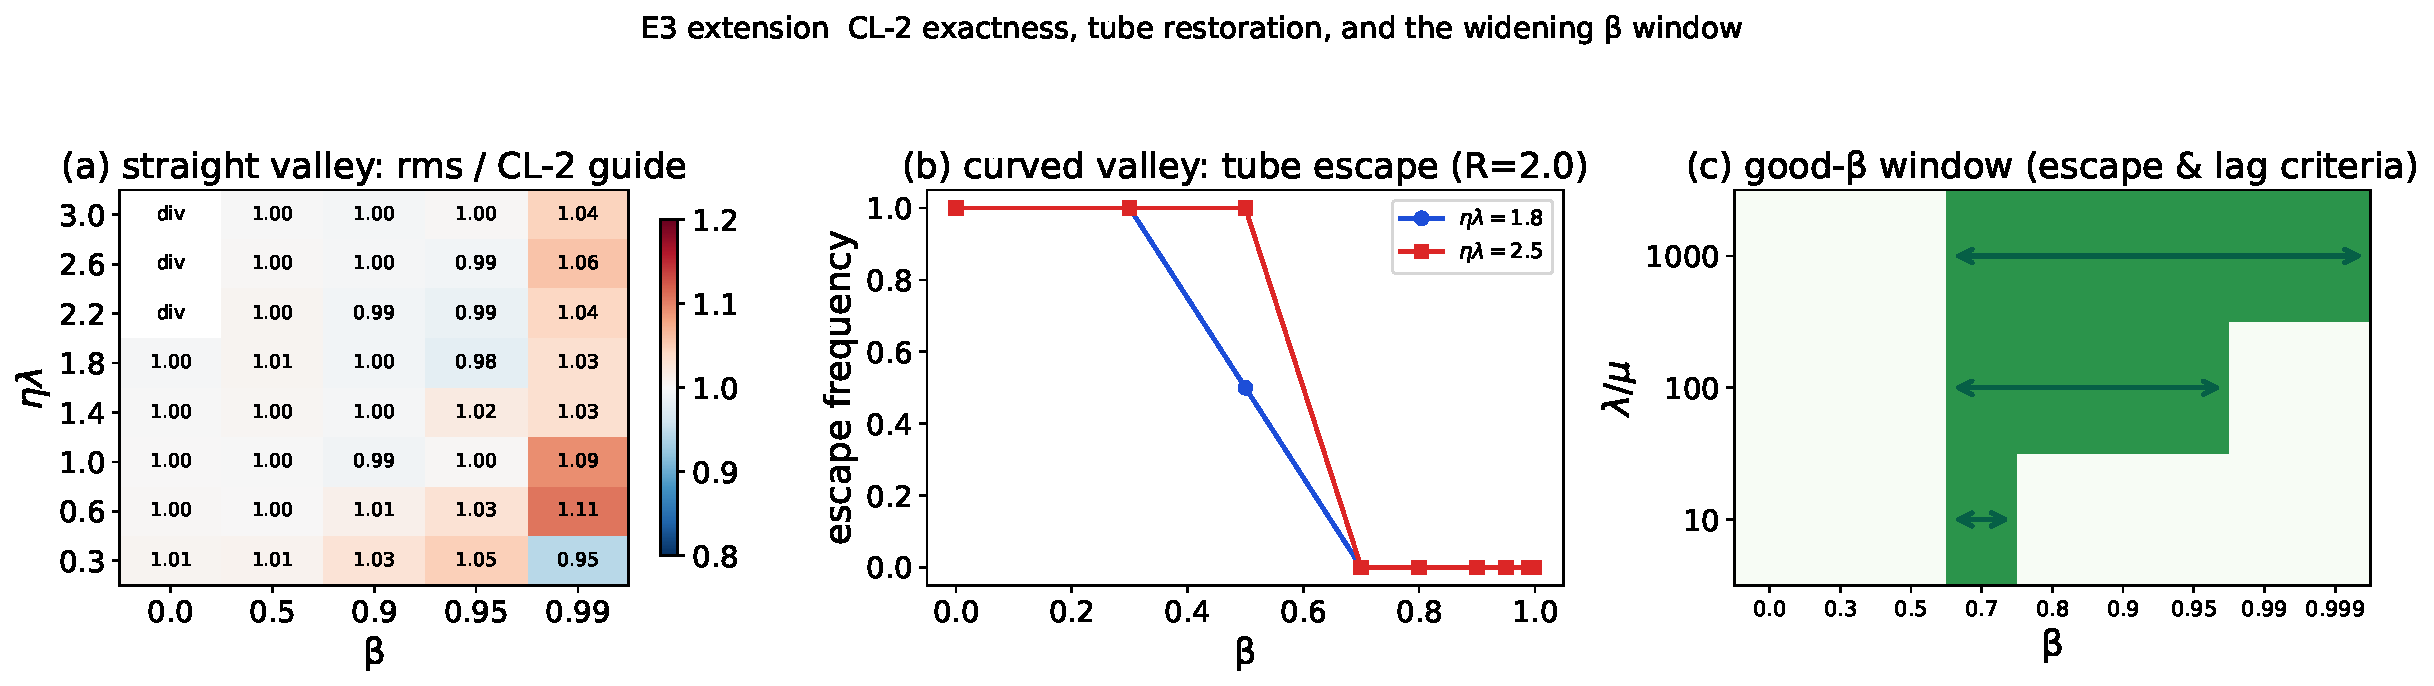
\includegraphics[width=\linewidth]{fig_e3_heatmap}
\caption{Closed-loop grid.
(a) straight valley, $\sigma=2$, $8$ seeds, $T=6000$: measured stationary rms over the \Cref{prop:variance} guide, per $(\eta\lambda,\beta)$ cell; cells beyond the \Cref{prop:stability} threshold marked ``div''.
(b) curved valley, $T=300$: tube-escape frequency versus $\beta$ at $\eta\lambda\in\{1.8,2.5\}$, $R=2$.
(c) $\beta$ window (shaded, arrow-spanned) versus conditioning $\lambda/\mu$ at $\eta\lambda=1.8$: escape frequency $\le0.25$ and mean river-following lag $\le1.25\times$ its per-conditioning minimum over the traveling horizon $3/(\eta\mu)$, $16$ seeds.
Source: run \texttt{cl2\_grid\_sweep\_el8\_b5\_seeds8}.}
\label{fig:e3heatmap}
\end{figure}

\section{Real-Network Diagnostics}
\label{sec:real}

We train a two-layer ReLU network full-batch by gradient descent on an ill-conditioned, non-realizable target $y=\sin(3\langle w,x\rangle)$, and record the first-layer weight gradient at each step.
At the learning rate $\eta=0.3$ the run sits at the edge of stability \citep{cohen2021edge}: the loss still descends ($0.51\to0.31$) while the gradient stream is dominated by a Nyquist oscillation.
The temporal high-frequency energy ratio is $0.994$ against a white-stream baseline of $0.406$, and the Frobenius spectral peak is exactly at $\omega=\pi$ (\Cref{fig:e6}).
Applying the EMA off-line suppresses the high band as $\Hmag{\pi}^2$ predicts and raises the buffer's alignment with the slow (mean) gradient as $\beta$ grows (\Cref{tab:e6}).
The structure is regime-dependent: at sub-critical $\eta$ the gradient stream is smooth (high-frequency energy ratio near zero), and at $\eta\gtrsim1$ the run diverges.
This is the river-valley hill of \Cref{sec:spectrum}, realized in a network at the edge of stability.

The structure is also time-dependent, in the way \Cref{lem:confinement} suggests.
Re-analysing the same run in sliding windows over the full stream (\Cref{fig:e6onset}), the windowed high-frequency energy ratio starts at $0.025$ and reaches $0.9$ only at step $200$, by which point $68\%$ of the total loss decrease has already happened; every later window sits above $0.98$.
The per-window alignment gain of the EMA buffer over the raw gradient is $+0.10$ before that onset and $+0.69$ after.
Before the iterate is confined, the steep-direction gradient \emph{is} the descent signal---low temporal frequency, nothing for the filter to remove---and the Nyquist hill appears only once confinement holds.
This reconciles the finding of \citet{li2025frequency} that high-frequency gradient content helps early and hurts late: filtering starts paying at confinement.

\begin{figure}[t]
\centering
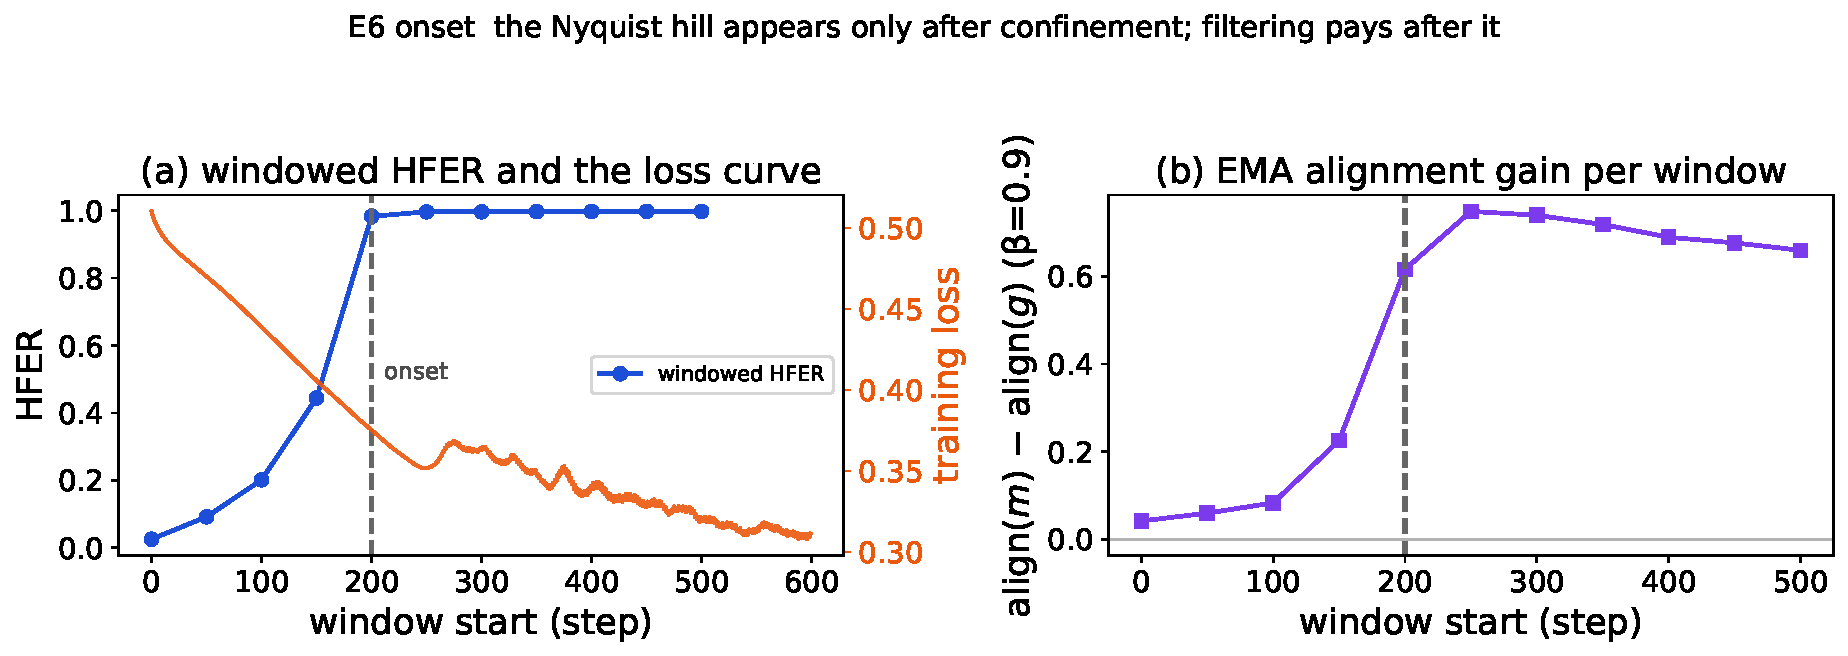
\includegraphics[width=0.86\linewidth]{fig_e6_onset}
\caption{Confinement onset (E6), windows of length $100$, stride $50$, over the full $600$-step stream.
(a) windowed HFER per window start, training loss on the right axis, onset (first window with HFER $\ge0.9$) dashed.
(b) per-window alignment gain $\Align_{\mathrm{slow}}(m)-\Align_{\mathrm{slow}}(g)$ at $\beta=0.9$ against the window-mean gradient, first $20$ in-window steps dropped as warm-up.
Source: run \texttt{mlp\_diagnostic\_trajectory\_cond120\_eta0p3\_T600}.}
\label{fig:e6onset}
\end{figure}

\begin{table}[t]
\centering
\caption{Real network at the edge of stability (E6): high-band momentum suppression ratio MSR and slow-gradient alignment $\Align_{\mathrm{slow}}(m)$ versus $\beta$, against the Nyquist guide $\Hmag{\pi}^2$.
Raw-gradient alignment is $0.261$.
Values from \texttt{metrics.json}.}
\label{tab:e6}
\begin{tabular}{lcccc}
\toprule
$\beta$ & $0.5$ & $0.9$ & $0.95$ & $0.99$\\
\midrule
MSR                       & $0.111$ & $0.00278$ & $0.000660$ & $0.0000253$\\
$\Hmag{\pi}^2$            & $0.111$ & $0.00277$ & $0.000657$ & $0.0000253$\\
$\Align_{\mathrm{slow}}(m)$& $0.362$ & $0.660$   & $0.732$    & $0.823$\\
\bottomrule
\end{tabular}
\end{table}

\begin{figure}[t]
\centering
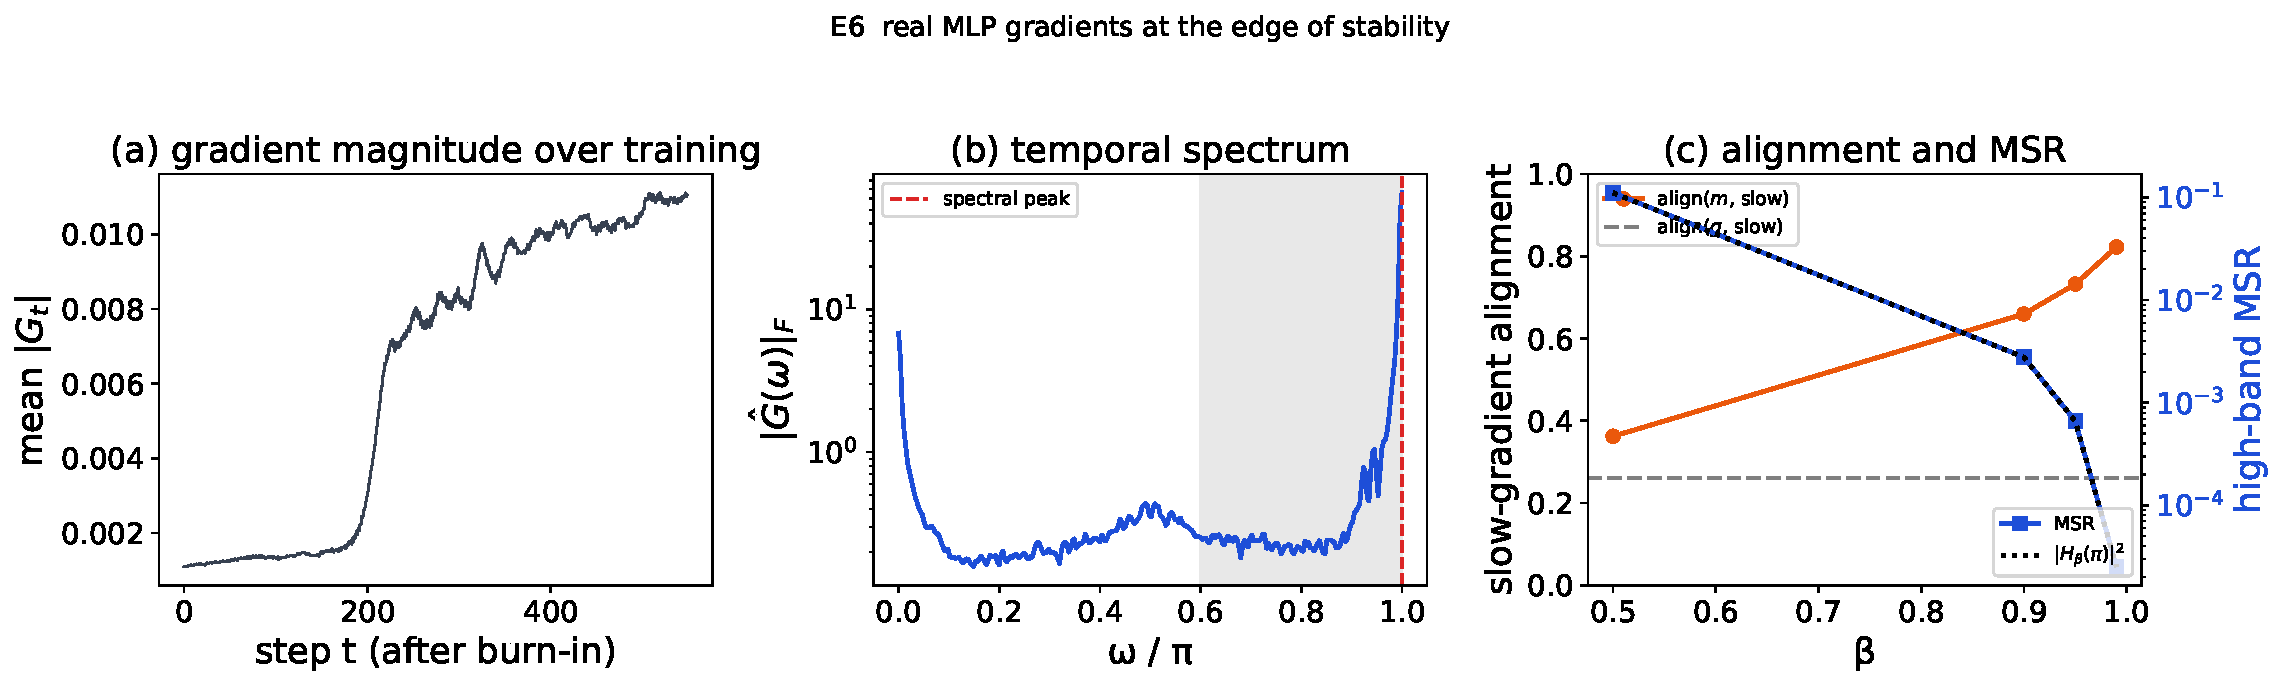
\includegraphics[width=\linewidth]{fig_e6_trajectory}
\caption{Real two-layer network at the edge of stability (E6), $\eta=0.3$, full-batch GD, $T=600$.
(a) mean magnitude of the first-layer gradient over training.
(b) temporal Frobenius spectrum, high band $\omega\ge0.6\pi$ shaded, dominant peak marked.
(c) slow-gradient alignment of the EMA buffer versus $\beta$ (left, with the raw-gradient baseline dashed) and high-band MSR with the $\Hmag{\pi}^2$ guide (right, log).
Source: run \texttt{mlp\_diagnostic\_trajectory\_cond120\_eta0p3\_T600}.}
\label{fig:e6}
\end{figure}

\section{Optimizer-Level Tests (E7)}
\label{sec:optimizer}

The mechanism claims predict where momentum pays off; E7 asks whether the mechanism metrics predict closed-loop \emph{performance} better than $\beta$ alone (\Cref{fig:e7}).
Closed-loop EMA momentum is run on five river-valley settings chosen so the best $\beta$ varies (straight at $\eta\lambda\in\{0.6,1.8\}$, curved at $\eta\lambda\in\{1.8,2.5\}$, and a doubled bend frequency; $\sigma=2$, $8$ seeds, $\beta\in\{0,0.5,0.8,0.9,0.95,0.99\}$).
The best $\beta$ ranges over $\{0.5,0.8,0.9,0.95\}$ across settings, and within a setting the loss is U-shaped in $\beta$, so the rank correlation of tail loss with $\beta$ is weak and sign-inconsistent (median absolute Spearman correlation $0.60$, sign flipping across settings).
A mechanism score---the within-setting rank of the buffer's hill energy plus the rank of its river-following lag, the two arms of \Cref{rem:tradeoff}---correlates at median Spearman correlation $+0.75$, winning in four of five settings; the exception is the benign $\eta\lambda=0.6$ setting, where the loss is flat in $\beta$ and all ranks are noise, itself the small-learning-rate reading of \Cref{prop:variance}.

The same contrast appears in the network of \Cref{sec:real}, trained closed-loop.
At $\eta=0.3$ the gradient stream is hill-dominated (HFER $0.99$) and the best $\beta$ improves the tail training loss over $\beta=0$ by $23\%$ ($0.241$ at $\beta=0.9$ vs $0.314$), with the U-shape closing again at $\beta=0.99$ ($0.314$); at $\eta=0.05$ the stream is smooth (HFER $0.02$), no $\beta$ improves the tail loss, and $\beta\le0.95$ changes it by under $1\%$ ($\beta=0.99$ costs $4\%$---the warm-up lag of a $199$-step memory in a $600$-step run).
The regime that determines whether momentum pays is identified by the stream's spectrum, not by $\beta$.
Finally, the Muon-style closed loop on the first layer ($\eta_o=0.02$, $\beta\in\{0.5,0.9,0.95\}$): at $\eta=0.3$, pre-polar beats post-polar on final training loss at every $\beta$ ($0.153$ vs $0.271$ at $\beta=0.95$) and on slow-gradient alignment of the update stream at every $\beta$---the closed-loop counterpart of \Cref{thm:filterfirst} and E5---and polar-only is worst ($0.298$).
Repeating the comparison at $\eta=0.05$, where the stream is smooth, the ordering dissolves: the median pre-to-post gap falls from $+0.22$ to $+0.07$ and its sign flips across $\beta$ (post-polar wins at $\beta=0.9$), with polar-only mid-pack ($0.108$).
Filter-first matters exactly where the stream is hill-dominated.

These are optimization claims, and on this task the held-out loss moves against them: at the edge of stability the cell with the lowest training loss ($\beta=0.9$) is the cell with the highest held-out loss, and post-polar beats pre-polar on held-out loss at every $\beta$ while losing on training loss.
Whether filtering removes update noise that acted as implicit regularization, or the $512$-sample synthetic task simply overfits, E7 does not distinguish; momentum's optimization gain need not be a generalization gain in this regime, an axis not modeled by the filtering theory.

\begin{figure}[t]
\centering
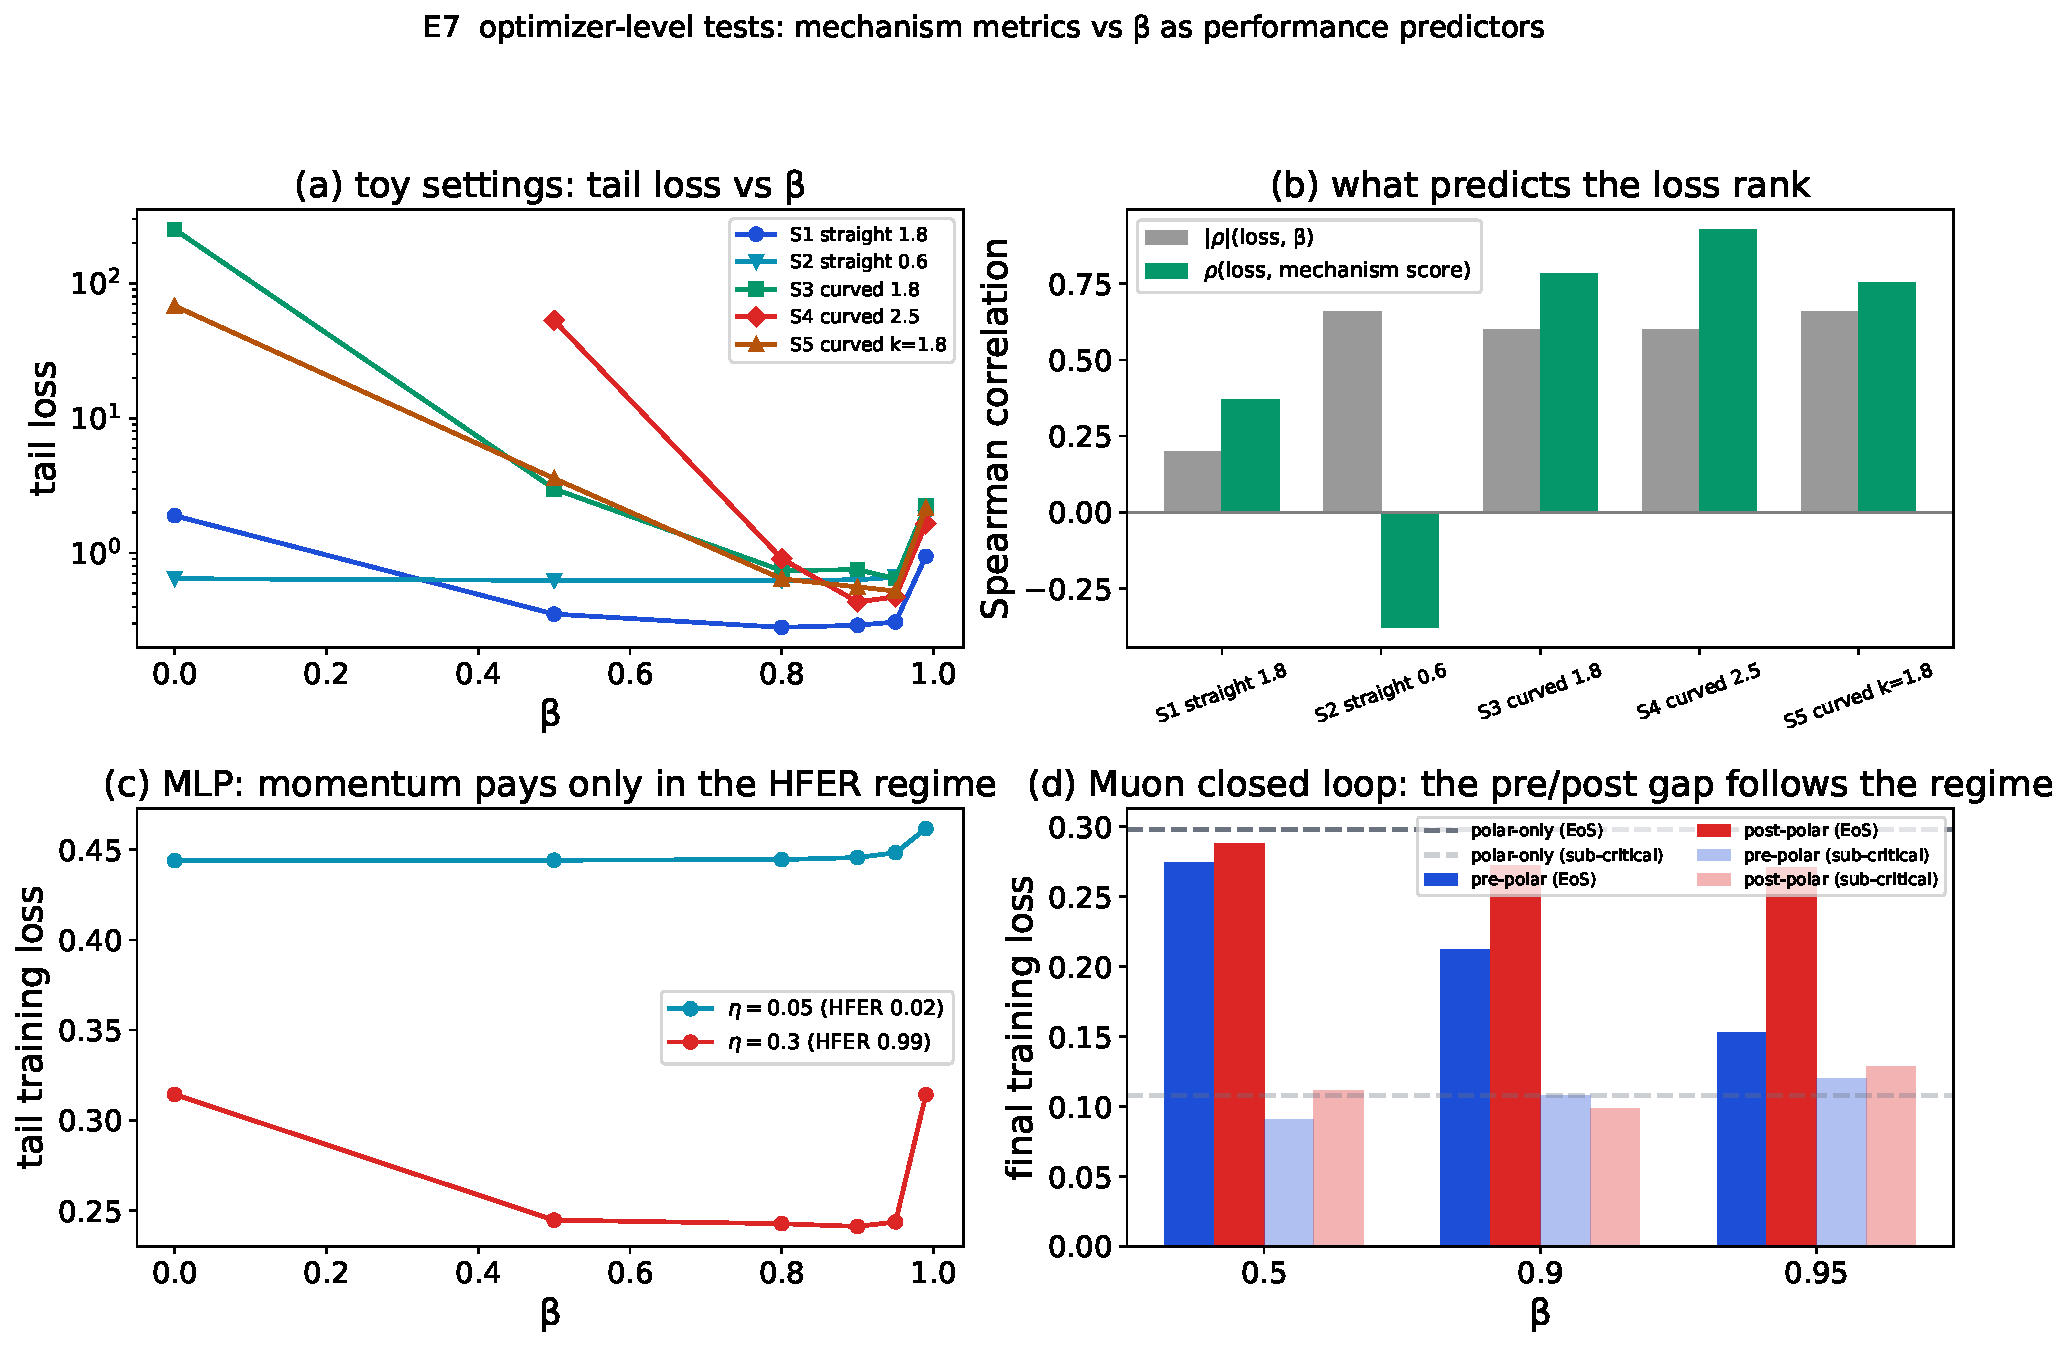
\includegraphics[width=0.98\linewidth]{fig_e7_optimizer}
\caption{Optimizer-level tests (E7).
(a) closed-loop EMA momentum tail loss versus $\beta$ (log) on the five toy settings, $\sigma=2$, $8$ seeds; diverged cells omitted.
(b) per-setting Spearman correlation of the tail-loss rank with $\beta$ (grey, absolute value) and with the mechanism score (green).
(c) the network of \Cref{sec:real} trained closed-loop: tail training loss versus $\beta$ at $\eta\in\{0.05,0.3\}$, each regime's stream HFER in the legend.
(d) Muon-style pre-polar versus post-polar on the first layer at $\eta=0.3$, $\eta_o=0.02$: final training loss by $\beta$.
Sources: runs \texttt{optimizer\_toy\_closedloop\_set5\_b6\_seeds8}, \texttt{optimizer\_mlp\_closedloop\_eta2\_b6\_muon3}.}
\label{fig:e7}
\end{figure}

\section{Mini-Batch Scale Transfer (E11)}
\label{sec:scale}

The remaining question is whether any of this survives real mini-batch training.
We drop Karpathy's nanoGPT into the codebase unmodified and train a $0.40$M-parameter character-level GPT (two blocks, $n_{\mathrm{embd}}=128$, block size $128$, batch $32$) on the tiny-Shakespeare corpus for $2000$ steps, under exactly the update rules of this paper: EMA-SGDM on all parameters, or the Muon-style variants of \Cref{eq:orders} on the last block's MLP expansion matrix with plain SGD elsewhere; no gradient clipping (a divergence guard stops runs instead, so instability is observed rather than masked), batch order fixed per seed across arms.
The probed matrix's per-step mini-batch gradient is recorded over a $256$-step mid-training window and analysed with the same measurements as every other experiment.

\subsection{Closed-loop sweep (E11)}
\label{sec:e11}
Three of the toy claims transfer, one transfers with a caveat, and one does not (\Cref{fig:e11}).
First, the regime map: the raw mini-batch gradient stream of the probed matrix is hill-dominated at every stable learning rate---HFER $0.821$, $0.823$, $0.838$ at $\mathrm{lr}=0.05$, $0.1$, $0.2$ against a white-stream baseline of $0.402$; the word \emph{hill} in this claim is earned by the decomposition of \Cref{sec:e12}.
Unlike the full-batch network of \Cref{sec:real}, there is no smooth sub-critical regime to find: mini-batch training holds the stream in the high band at every learning rate we could run, and E12 locates that high band in the mean-loss gradient's response on the top curvature directions, with the layer-restricted spectrum far below the edge.
Second, the momentum benefit follows the regime scaling of \Cref{cor:hillloss}: the best-$\beta$ improvement in tail training loss over $\beta=0$ rises $0.8\%$, $3.5\%$, $11.9\%$, $21.8\%$ across the four learning rates.
The best cell of the whole sweep is $(\mathrm{lr}=0.4,\beta=0.95)$ at $1.946$---a learning rate at which $\beta=0$ diverges on one of three seeds and its surviving runs sit among the worst cells ($2.488$).
The stabilized regime exists at scale, though the divergence boundary is seed-marginal rather than sharp at this batch size ($\beta=0.5$ survives with visible instability spikes).
Third, filter-first: pre-polar beats post-polar at every $\beta$ at $\mathrm{lr}=0.05$ and at two of three at $\mathrm{lr}=0.2$, with polar-only mid-pack; the gaps (median $+0.02$, $+0.03$) are small against the diagnostic network's, consistent with both streams being hill-dominated and the probed layer being one of many.
What does not transfer: the mechanism score that ranked the toy cells (\Cref{sec:optimizer}) does not resolve the small within-row loss spreads here (median within-row rank correlation $-0.09$ from a single probe seed).
Identifying the regime is where the stream metrics earn their keep at scale; ranking $\beta$ within a regime is not.
Finally, the axis E7 could not separate: on this corpus the held-out loss tracks the training loss (rank correlation $0.90$ over all cells; the best training cell is also the best validation cell)---the optimization gain is not paid back in generalization here, so the anti-correlation of \Cref{sec:optimizer} was the synthetic task's overfitting axis, as stated there.

\begin{figure}[t]
\centering
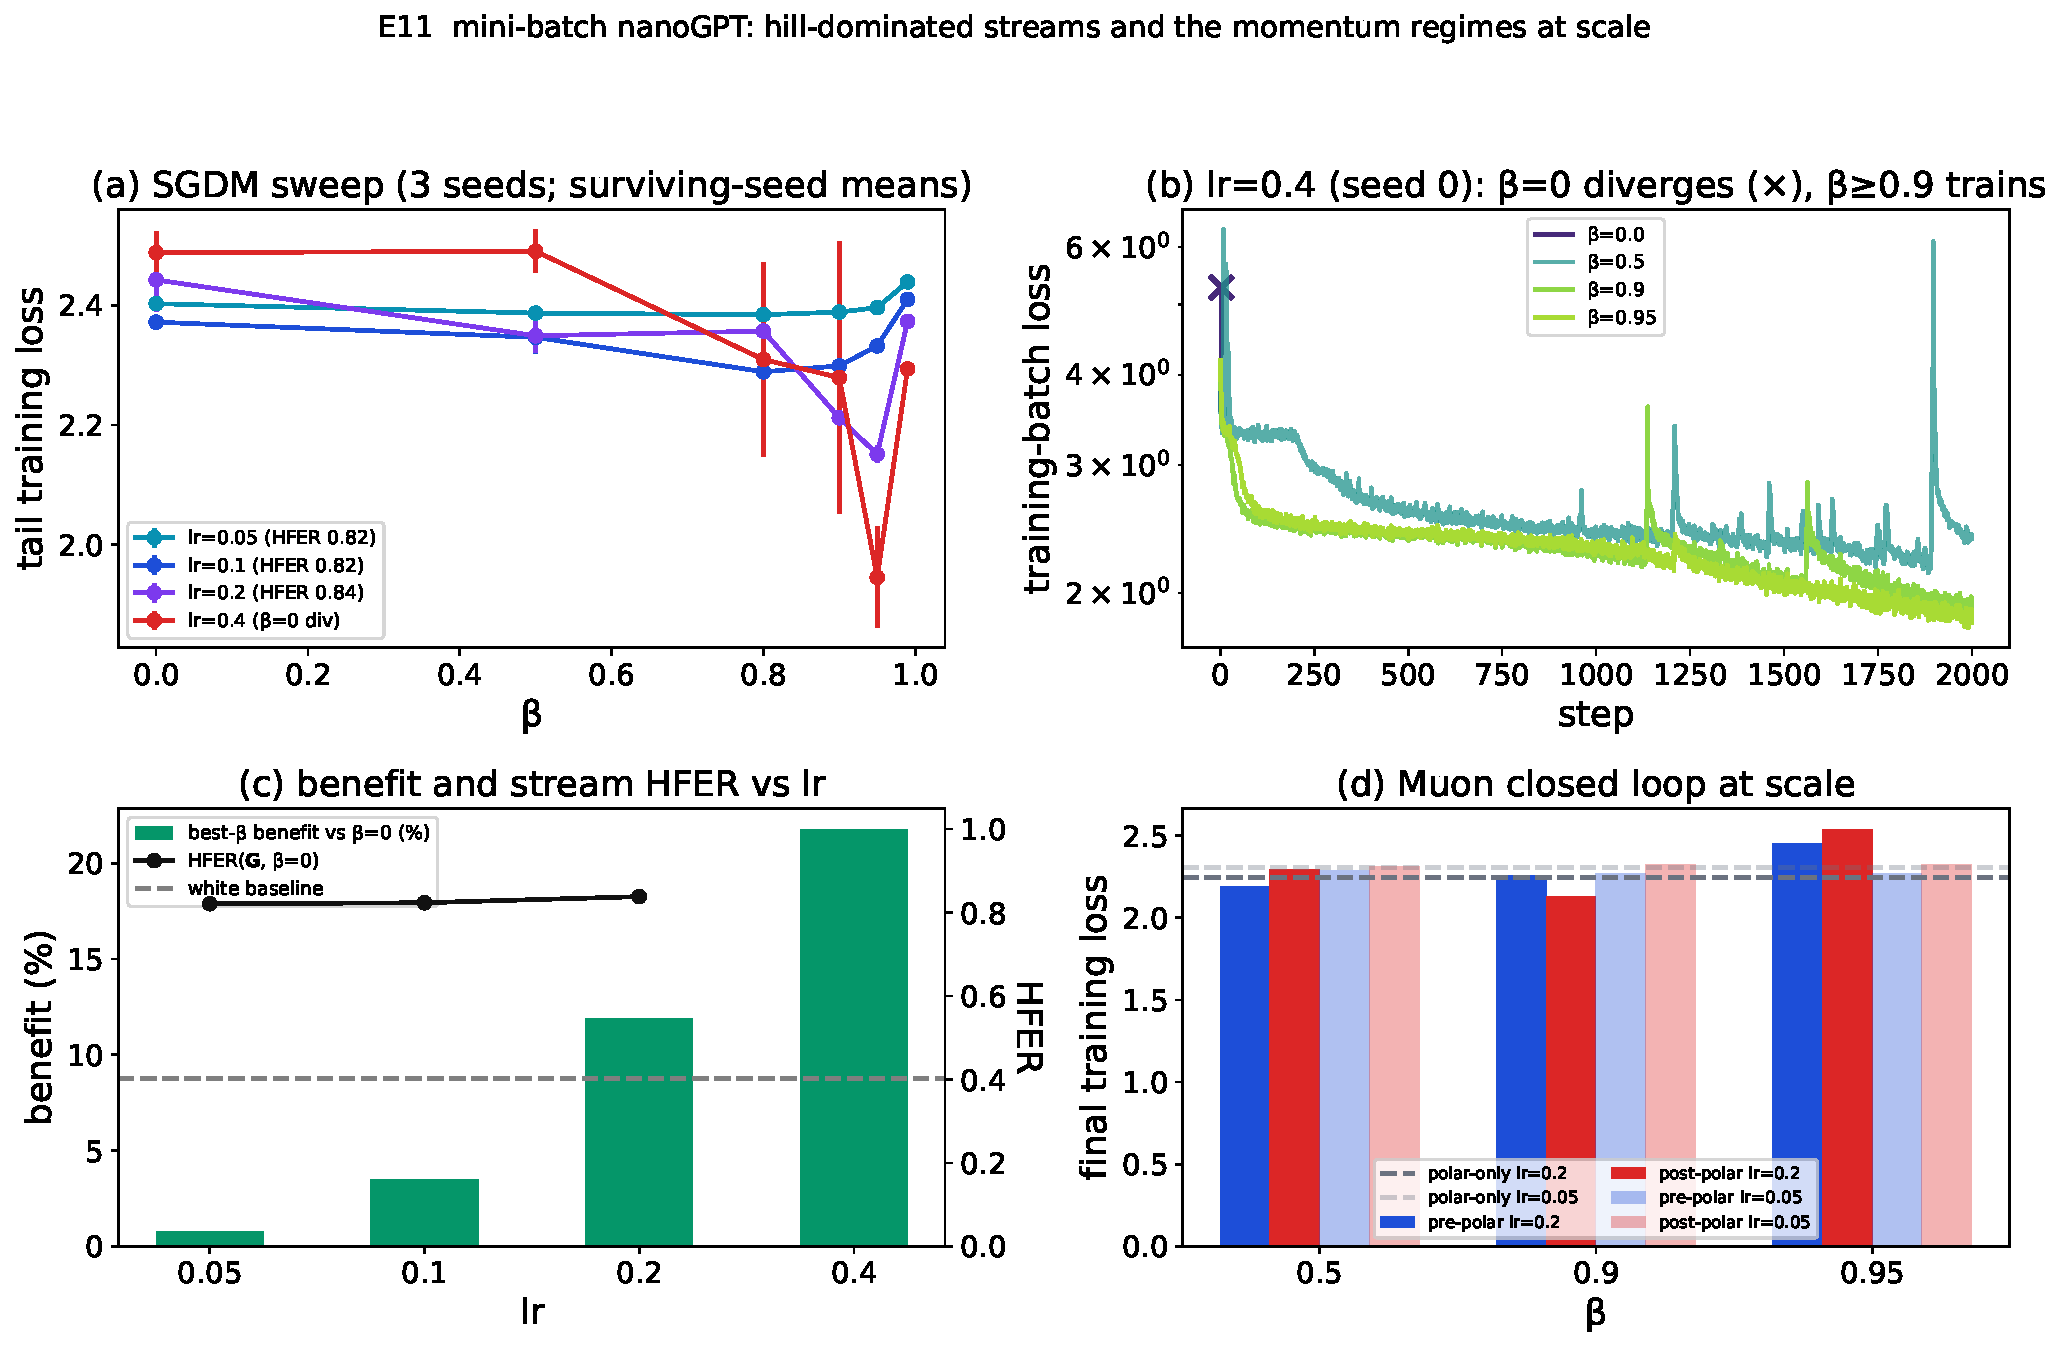
\includegraphics[width=\linewidth]{fig_e11_scale}
\caption{Mini-batch nanoGPT (E11): $0.40$M-parameter character-level GPT (upstream nanoGPT, unmodified), shakespeare\_char, batch $32\times128$, $T=2000$, EMA-SGDM on all parameters, no gradient clipping, $3$ seeds with seed-fixed batch order; probe window steps $1200$--$1455$ of the last block's MLP expansion gradient.
(a) tail training loss (mean of the last $200$ steps) versus $\beta$ per learning rate; surviving-seed means, error bars seed std; legend entries carry the raw-stream HFER at $\beta=0$.
(b) seed-0 loss curves at $\mathrm{lr}=0.4$; $\times$ marks the $\beta=0$ divergence.
(c) best-$\beta$ benefit over $\beta=0$ (bars) and HFER$(\Gbf,\beta{=}0)$ (line) versus learning rate, white-stream baseline dashed.
(d) Muon pre-/post-polar final loss at background $\mathrm{lr}\in\{0.2,0.05\}$, $\eta_o=0.02$, polar-only dashed per lr.
Source: run \texttt{nanogpt\_closedloop\_lr4\_b6\_seeds3\_T2000}.}
\label{fig:e11}
\end{figure}

\subsection{Hill oscillation or sampling noise? (E12)}
\label{sec:e12}
A high HFER alone does not earn the word \emph{hill}: high-band energy could in principle be sampling noise rather than landscape response.
E12 separates the two along both axes the theory names.
At each probe step a large-batch estimate $\bar g^{\mathrm{LB}}_t$ ($1024$ sequences, $32\times$ the training batch) of the mean-loss gradient at the visited iterate splits the recorded stream as $g^{\mathrm{mb}}_t=\bar g^{\mathrm{LB}}_t+\xi^{\mathrm{res}}_t$, and the top-$16$ eigenpairs of the probed matrix's restricted Hessian are estimated at the window midpoint (block power iteration, residuals at most $0.012$ on the top four directions; plain SGD, so the stream is the raw one; $3$ seeds per stable learning rate).
The design logic: a temporally independent residual has a flat spectrum whatever its spatial structure, so HFER above the white baseline must come from the state stream---the mean-loss gradient along the visited iterates, which is what the closed loop of \Cref{thm:spectrum} describes.

The split is one-sided (\Cref{fig:e12}).
The sampling residual is white: HFER $0.400$, $0.404$, $0.409$ at $\mathrm{lr}=0.05$, $0.1$, $0.2$, against the white baseline $0.402$.
The state stream's HFER exceeds the raw stream's in every run (seed means $0.84$--$0.92$ against $0.82$--$0.91$), and the high-band state share (\Cref{sec:measurements}) is $0.83$, $0.84$, $0.93$.
Accounting for the raw stream's high band directly, the state stream contributes $0.72$, $0.73$, $0.86$, the positive state--residual cross terms $0.13$, $0.13$, $0.07$, and the residual the remaining $0.15$, $0.14$, $0.07$; the large-batch estimator's own sampling error ($1/32$ of the residual's energy) biases the state's part \emph{down}.
Geometrically, the top-$16$ curvature directions---$2.4\times10^{-4}$ of the $65{,}536$ dimensions---carry $0.92$, $0.88$, $0.82$ of the state stream's high-band energy, and the in-subspace HFER exceeds the out-of-subspace HFER at every learning rate ($0.88$--$0.94$ against $0.56$--$0.81$).
The mini-batch high band is hill oscillation in the measured sense: mean-loss gradient response, concentrated on top curvature directions, with white sampling noise on top---not a stream that momentum merely denoises.
One number scopes the reading: the restricted top eigenvalue sits at $\eta\lambda\in[0.21,0.42]$ (seed means; per-run range $0.06$--$0.47$), far below the edge.
Restriction to one layer bounds network sharpness only from below (eigenvalue interlacing), so the oscillating mode is a network-level object whose layer block aligns with the layer's top restricted curvature; the restricted $\lambda_i$ are therefore not the per-direction constants of \Cref{thm:spectrum}, and E12 reads them only as alignment evidence.

\begin{figure}[t]
\centering
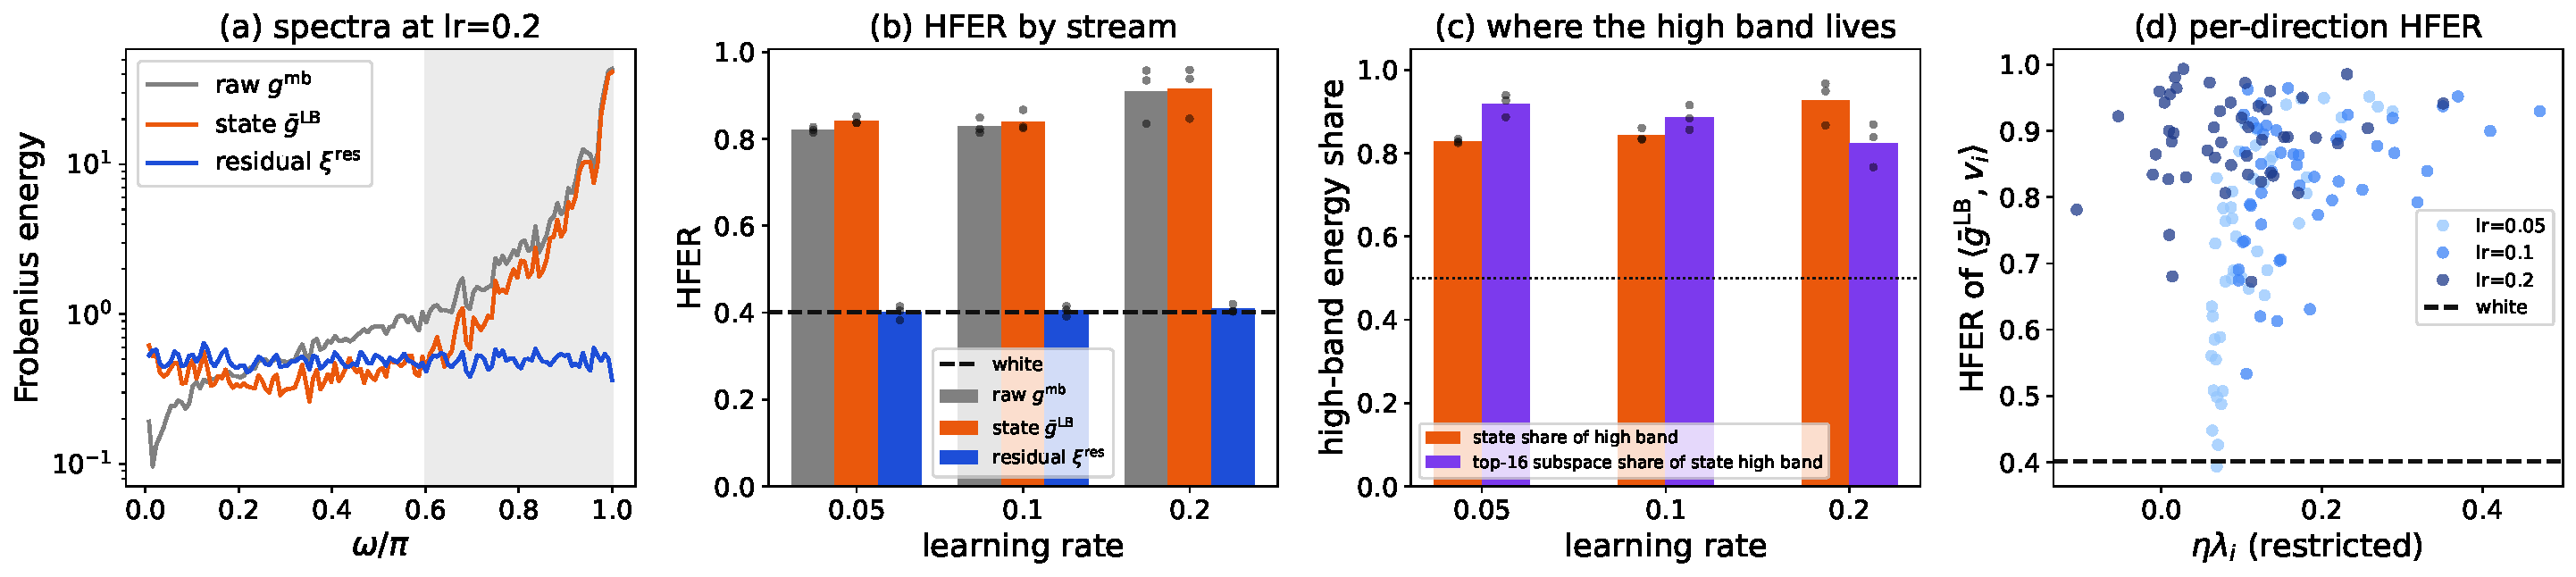
\includegraphics[width=\linewidth]{fig_e12_decomp}
\caption{Decomposition of the mini-batch stream (E12), nanoGPT probe window as in \Cref{fig:e11}, plain SGD, $3$ seeds, large-batch size $1024$, $k=16$ eigenpairs.
(a) per-frequency Frobenius energy of $g^{\mathrm{mb}}$, $\bar g^{\mathrm{LB}}$, $\xi^{\mathrm{res}}$ at $\mathrm{lr}=0.2$, seed mean (log).
(b) HFER of the three streams per learning rate, white baseline dashed.
(c) high-band state share and, of the state stream, the share captured by the top-$16$ curvature subspace, per learning rate.
(d) per-direction HFER of the state stream's coefficient series against $\eta\lambda_i$ (restricted eigenvalues), all learning rates and seeds, white baseline dashed.
Source: run \texttt{nanogpt\_decomp\_lr3\_seeds3\_LB1024\_k16}.}
\label{fig:e12}
\end{figure}

\section{Discussion}
\label{sec:discussion}

The three views of momentum coincide once it is read as a temporal filter.
Acceleration is the DC-pass behaviour $\Hmag{0}=1$ together with the effective step gain along persistent directions; denoising is the $1/\Teff$ attenuation of the broadband noise floor; and momentum additionally attenuates \emph{structured} high-frequency gradient components, of which the river-valley hill is the canonical example.
\Cref{thm:filter} ties these together with explicit constants at the stream level; \Cref{prop:stability,prop:variance} carry them to the trajectory, where the benefit is a large-learning-rate effect under sustained excitation and the deterministic transient remains the caveat; and \Cref{prop:forced} completes the trajectory story frequency by frequency---removed at Nyquist, neutral in the passband, amplified at the loop's own mode---with E13 confirming all three arms on parameter-free guides.
\Cref{rem:tradeoff} and \Cref{rem:window} turn them into a design statement: the optimum $\beta$ balances high-frequency attenuation $\rhohigh(\beta)$ against low-frequency distortion $\epslow(\beta)$, within a window that widens with the valley conditioning and narrows with the river curvature.
The direct sweep (E9) measures the improvement side of this statement at the predicted $\eta\lambda/2$; the curved valley (E2), the instantaneous-target reading of E3, the regime map (E8), and the bend-frequency sweep (E10) show the window side---its floor now predicted by \Cref{prop:curved}---including the closed-loop caveat that curvature is paid partly in river speed rather than lag.
On schedules, E7's schedule arm sharpens the reading: every arm whose $\beta$ prefix sits below the confinement floor---the smallest $\beta$ that keeps the trajectory in the tube---loses badly (a linear ramp from $0$ by a factor $15$ against fixed $\beta=0.9$; thirty steps at $\beta=0$ before stepping to $0.9$ by a factor $118$), while floor-respecting warmup wins outright (a ramp from $0.7$ to $0.95$ beats every fixed $\beta$).
Trajectory-triggered raises close the loop on this reading: starting at the floor, a confinement detector (ten consecutive in-tube steps) or a gradient-only proxy (the hill-gradient sign-flip fraction) fires at step ${\approx}11$ and lands with the fixed-$\beta$ arms ($0.83$ and $0.74$ against $0.75$ at fixed $\beta=0.9$), while the same detector started below the floor fires only at step ${\approx}201$ and loses by two orders of magnitude: adaptivity does not rescue a sub-floor start.
The confinement onset (E6) supports raising $\beta$ once the iterate is confined; when to raise $\beta$ is a confinement question, not a clock question---and from where, the floor; among floor-respecting schedules the gradual ramp remains the best arm.
\citet{shen2026muon} schedule the complementary control---the direction map, switched from the polar factor to AdamW at a fixed iteration; whether that switch is likewise a confinement question rather than a clock question, and how the two schedules compose, are untested.

\paragraph{Limitations.} The closed-loop propositions are proved for the linear (straight-valley) hill; the curved valley now has the frozen-coefficient reduction of \Cref{prop:curved}---exact for linear floors and predictive for E10's confinement floors---but a global curved-valley theorem remains open, and the reduction's validity margin $k\vriv\,\Teff\lesssim1$ is itself the window's top edge.
\Cref{thm:filterfirst,thm:bandlimited,cor:bandenergy} are statements about the buffer feeding the direction map---the honest scope for Muon-class updates---not nonlinear trajectory theorems, and they exclude Nesterov momentum, as does \citet{li2026denoise}; the Muon comparisons here probe one matrix in small models, not practical Muon training (Newton--Schulz orthogonalization, all matrix layers, tuned baselines).
The real-network evidence is one small full-batch network (E6, E7) and one $0.40$M-parameter mini-batch transformer (E11--E12): the hill-dominated stream---now decomposition-verified---the regime scaling of the benefit, the (seed-marginal) shifted stability boundary, and the filter-first ordering persist at that scale, while the within-regime mechanism-score ranking does not.
\Cref{prop:variance} assumes additive, state-independent white noise, which mini-batch noise is not: E12 verifies the temporal whiteness of the sampling residual at this scale, not state-independence or isotropy, so the closed-form constants remain model statements there.
Production scale, Adam-preconditioned updates, learning-rate schedules, and trajectory-level behavior of the \Cref{rem:mapscope} family remain untested, and are the runs the Integration Contract makes cheap.

\bibliography{references}
\bibliographystyle{abbrvnat}

\end{document}
